\chapter{Systematic uncertainties}
\label{chap:prod:syst}

Each experimental measurement of the double-differential cross-section defined 
in \cref{eqn:prod:introduction:differential_cross_section} is comprised of a 
central value and a set of uncertainties.
One uncertainty is \emph{statistical}, and is taken to be the uncertainty on 
the prompt signal yield $N(\HcTof)$, as measured in the fitting procedure 
described in \cref{chap:prod:fitting}.
The second uncertainty is the \emph{systematic} uncertainty, which quantifies 
all other sources of experimental accuracy.
This section will describe the individual components of this uncertainty, how 
they arise and how their values are estimated, and will finish with a summary 
stating how the components are combined as a single number.

In the discussion of systematic uncertainties, it is important to consider the 
correlations of the uncertainties both between \pTy\ bins and between charm 
hadrons.
Uncertainties that are fully correlated, with a correlation coefficient $\rho$ 
equal to 1, cancel in ratios.
In addition, the quantification of the goodness-of-fit of a fit to the 
cross-section measurements, as done by theorists, can change significantly when 
correlated are accounted for.
In what follows, the range of correlations of each uncertainty between bins and 
between charm hadrons will be given, with a summary presented in 
\cref{chap:prod:syst:correlations}.

The systematic uncertainties are treated as nuisance parameters of the 
cross-section measurement, being propagated as an additive parameter on the 
respective term they relate to.
The nuisance parameters are modelled as \aclp{PDF} in the framework of \acl{MC} 
error propagation, as described in \cref{chap:prod:introduction:uncertainties}.
Typically, the \ac{PDF} is a normal distribution with a mean of zero and a 
width corresponding to the size of the systematic variation being assessed, but 
the exact form will be given alongside the description of the uncertainty.

\section{Finite \acl{MC} sample size}
\label{chap:prod::syst:mcstat}

The Monte Carlo samples used to estimate the acceptance, reconstruction, and 
selection efficiencies are of a finite size, and so the computed efficiencies 
carry a non-zero statistical uncertainty.
This is propagated to the cross-section measurements as a systematic 
uncertainty.
As the set of \ac{MC} events is unique for each \pTy\ bin and mode, this 
systematic uncertainty is fully uncorrelated between bins and between decay 
modes.
As discussed in \cref{chap:prod:effs:tot}, the posteriori probability 
for the estimated efficiency is described by the beta distribution, and so the 
corresponding nuisance parameter is modelled by this distribution.

The resulting systematic uncertainties, relative to the central value of the 
cross-section measurement, are given in 
\cref{tab:prod:syst:mc:stat:D0ToKpi,tab:prod:syst:mc:stat:DpToKpipi} for 
\DzToKpi\ and \DpToKpipi.

\section{\acl{MC} modelling}
\label{chap:prod:syst:mc}

If the simulated data does not correctly model the selection variables, the 
selection efficiencies that are evaluated with \ac{MC}, described in 
\cref{chap:prod:effs:sel}, will be incorrect.
To assess the accuracy of the \acl{MC} modelling, signal distributions are 
extracted from the data using the \sPlot\ method~\cite{Pivk:2004ty} and are 
compared to the \ac{MC}.
As the definition of the selection efficiency does not include the effects of 
the \ac{PID} selection, the distributions of the real data are corrected for 
the \ac{PID} efficiency by a per-decay weighting.
The signal distributions in data are only available after the selection has 
been applied, and so the same selection is also applied to the simulated data 
(with the exception of the \ac{PID} requirements).
Comparisons of an example set of variables used in the \DzToKpi\ and 
\DpToKpipi\ selections are shown in 
\cref{fig:prod:syst:mc:D0ToKpi,fig:prod:syst:mc:DpToKpipi}, integrated across 
all \pTy\ bins for visualisation.
The agreement is generally good.

To quantify the effect of the mis-modelling of the selection efficiencies, the 
following procedure is performed for each selection variable $x$:
\begin{enumerate}
  \item Find the cut value $y$ on $x$ which rejects half of the selected 
    simulated data;
  \item Apply the cut value $y$ on $x$ to the \emph{real data}, counting the 
    number of signal candidates passing the requirement as the sum of signal 
    weights divided by the \ac{PID} selection efficiencies
    \begin{equation}
      N_{\text{Passed}} = \sum_{i}^{N} I(i) \frac{%
        w_{i,\text{signal}}
      }{%
        \eff_{i,\text{PID}}
      },
    \end{equation}
    where $I(i)$ is 1 if the value of $x$ for the $i$th event passes the 
    requirement $y$ on $x$, and is zero otherwise;
  \item The efficiency-corrected signal yield corresponding to the requirement 
    on $x$ is $2N_{\text{Passed}}$, which should equal the number of signal 
    candidates before the requirement $y$, if the \ac{MC} describes the data.  
    The quantity
    \begin{equation}
      \Delta = 2N_{\text{Passed}} - \sum_{N}^{i} \frac{w_{i,\text{signal}}}{\effpid},
      \label{eqn:prod:syst:mc:eff_diff}
    \end{equation}
    is then a handle on the mis-modelling of the data in the \ac{MC}.
\end{enumerate}
This procedure is repeated in every \pTy\ bin, for a total of $N_{\pT} \cdot 
N_{\rapidity} \cdot N_{\text{variables}}$ values of $\Delta$.

To account for correlations between variables, which may lead to 
double-counting of the mis-modelling if neglected, the procedure is repeated 
in ten thousand pseudo-experiments per selection variable.
For each trial, each candidate is sampled $n$ times from the real data, with 
$n$ being sampled from a Poisson distribution of mean 1.
The total systematic uncertainty on the efficiency-corrected signal yield due 
to \ac{MC} mis-modelling is the mean of the set of ten thousand values of $\Delta$, as defined in \cref{eqn:prod:syst:mc:eff_diff}.

The value of $\Delta$ for a given variable in a single \pTy\ bin is usually not 
statistically significant, but the integration of the $\Delta$ values all over 
\pTy\ values can be, and so a difference is evaluated for all \pTy\ bins as 
such.
The relative uncertainty on the efficiency-corrected yield $N/\eff$ is the 
difference integrated across all \pTy\ divided by it's uncertainty.
This is given for all modes in \cref{tab:prod:syst:mc:modelling}.

\begin{figure}
  \begin{subfigure}{0.3\textwidth}
    \centering
    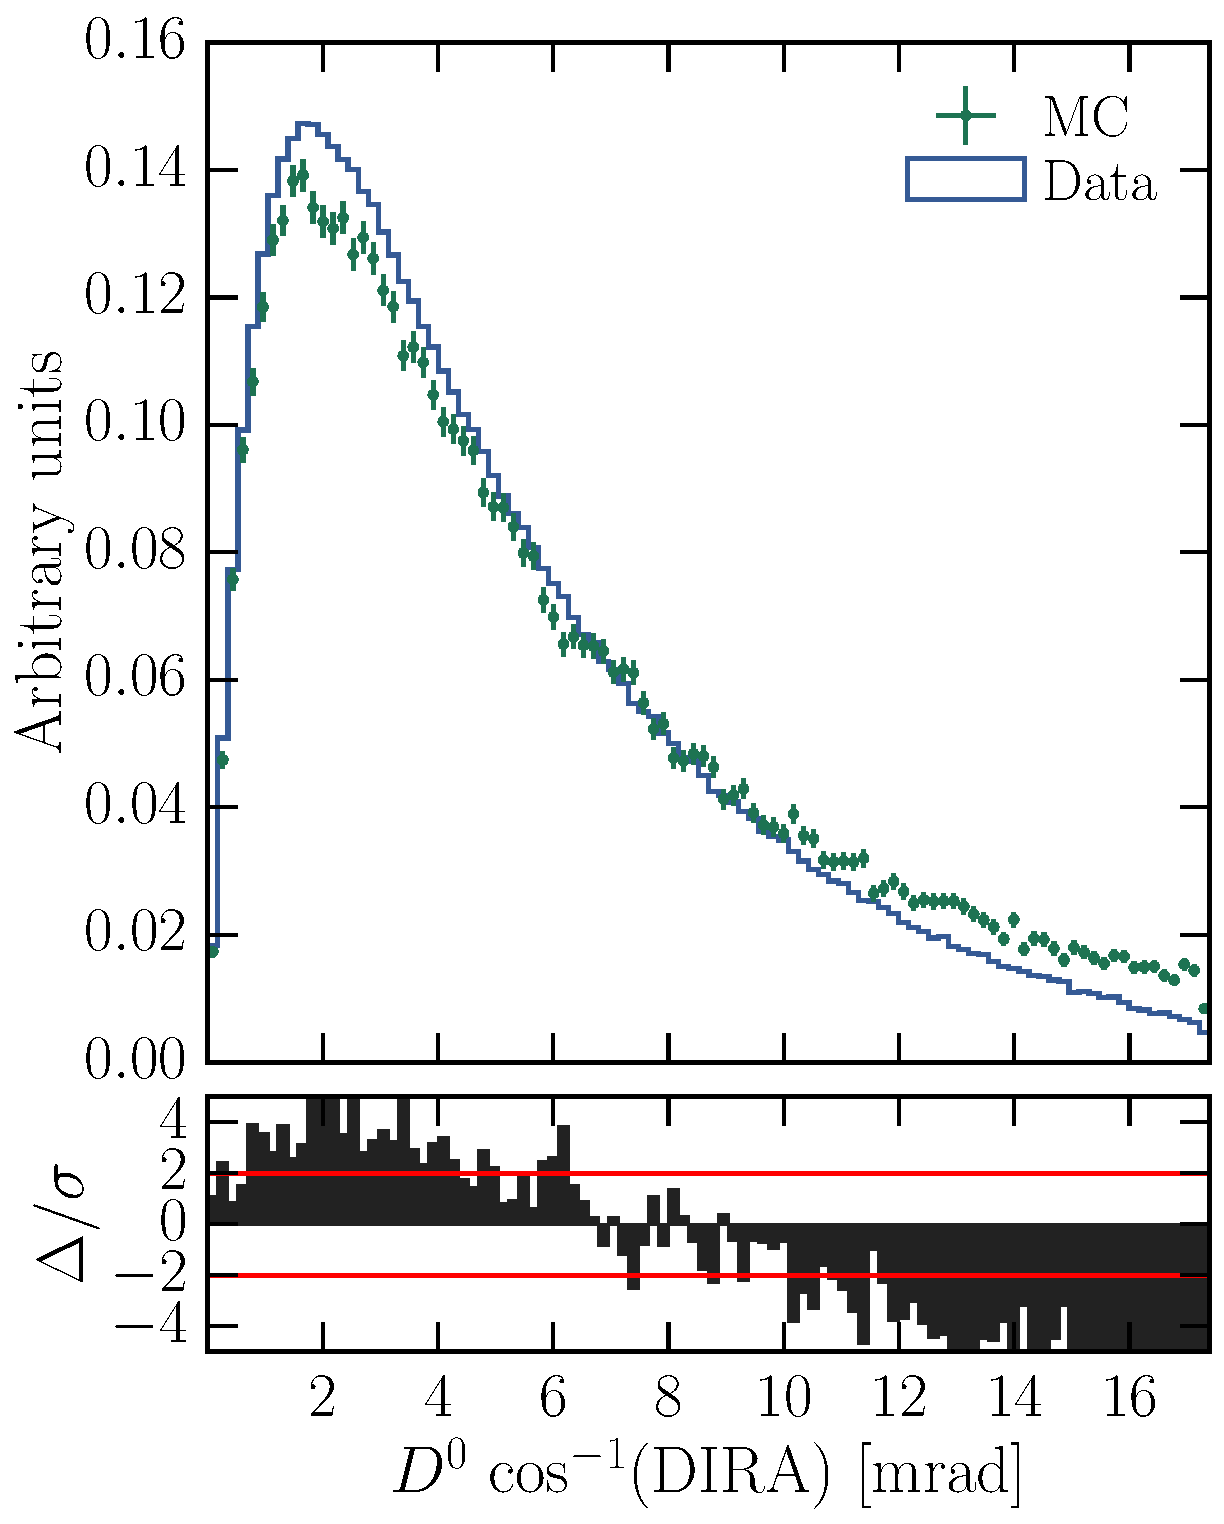
\includegraphics[width=\textwidth]{production/systematics/data_mc/D0_DIRA_OWNPV}
    \caption{\PDzero \ac{DIRA}}
  \end{subfigure}
  \begin{subfigure}{0.3\textwidth}
    \centering
    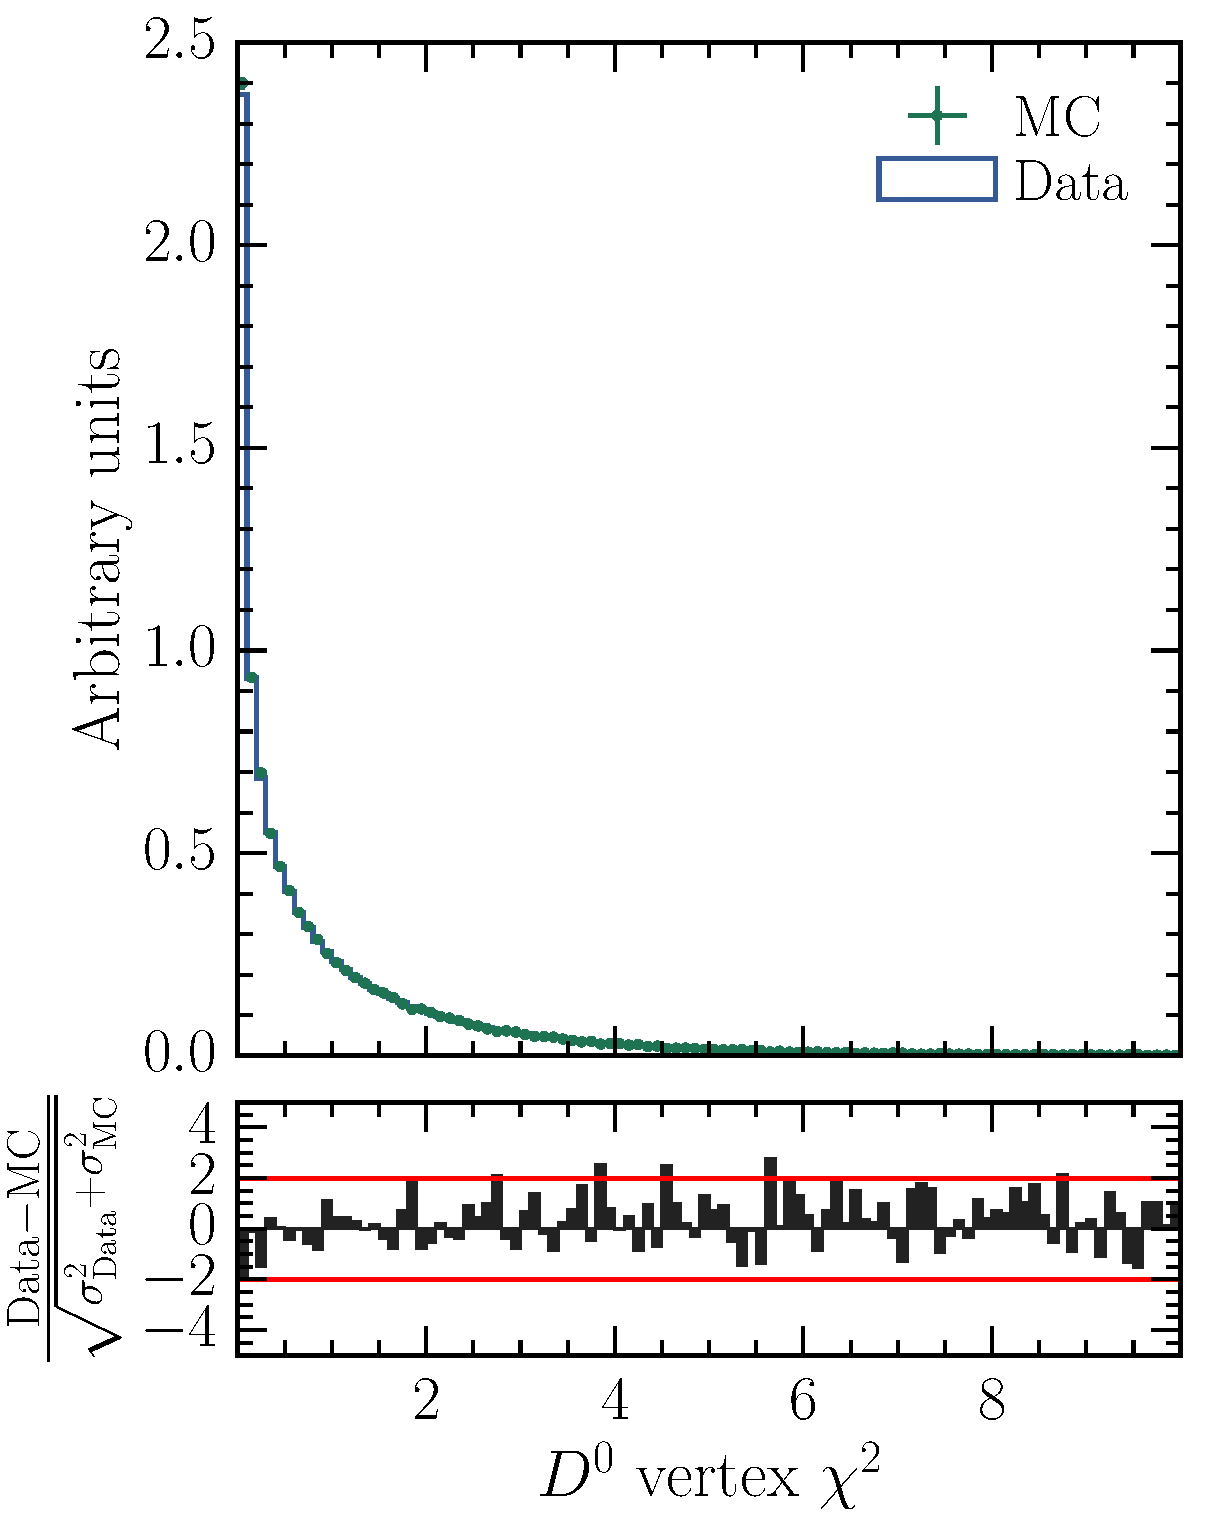
\includegraphics[width=\textwidth]{production/systematics/data_mc/D0_ENDVERTEX_CHI2-D0_ENDVERTEX_NDOF}
    \caption{\PDzero vertex \chisq}
  \end{subfigure}
  \begin{subfigure}{0.3\textwidth}
    \centering
    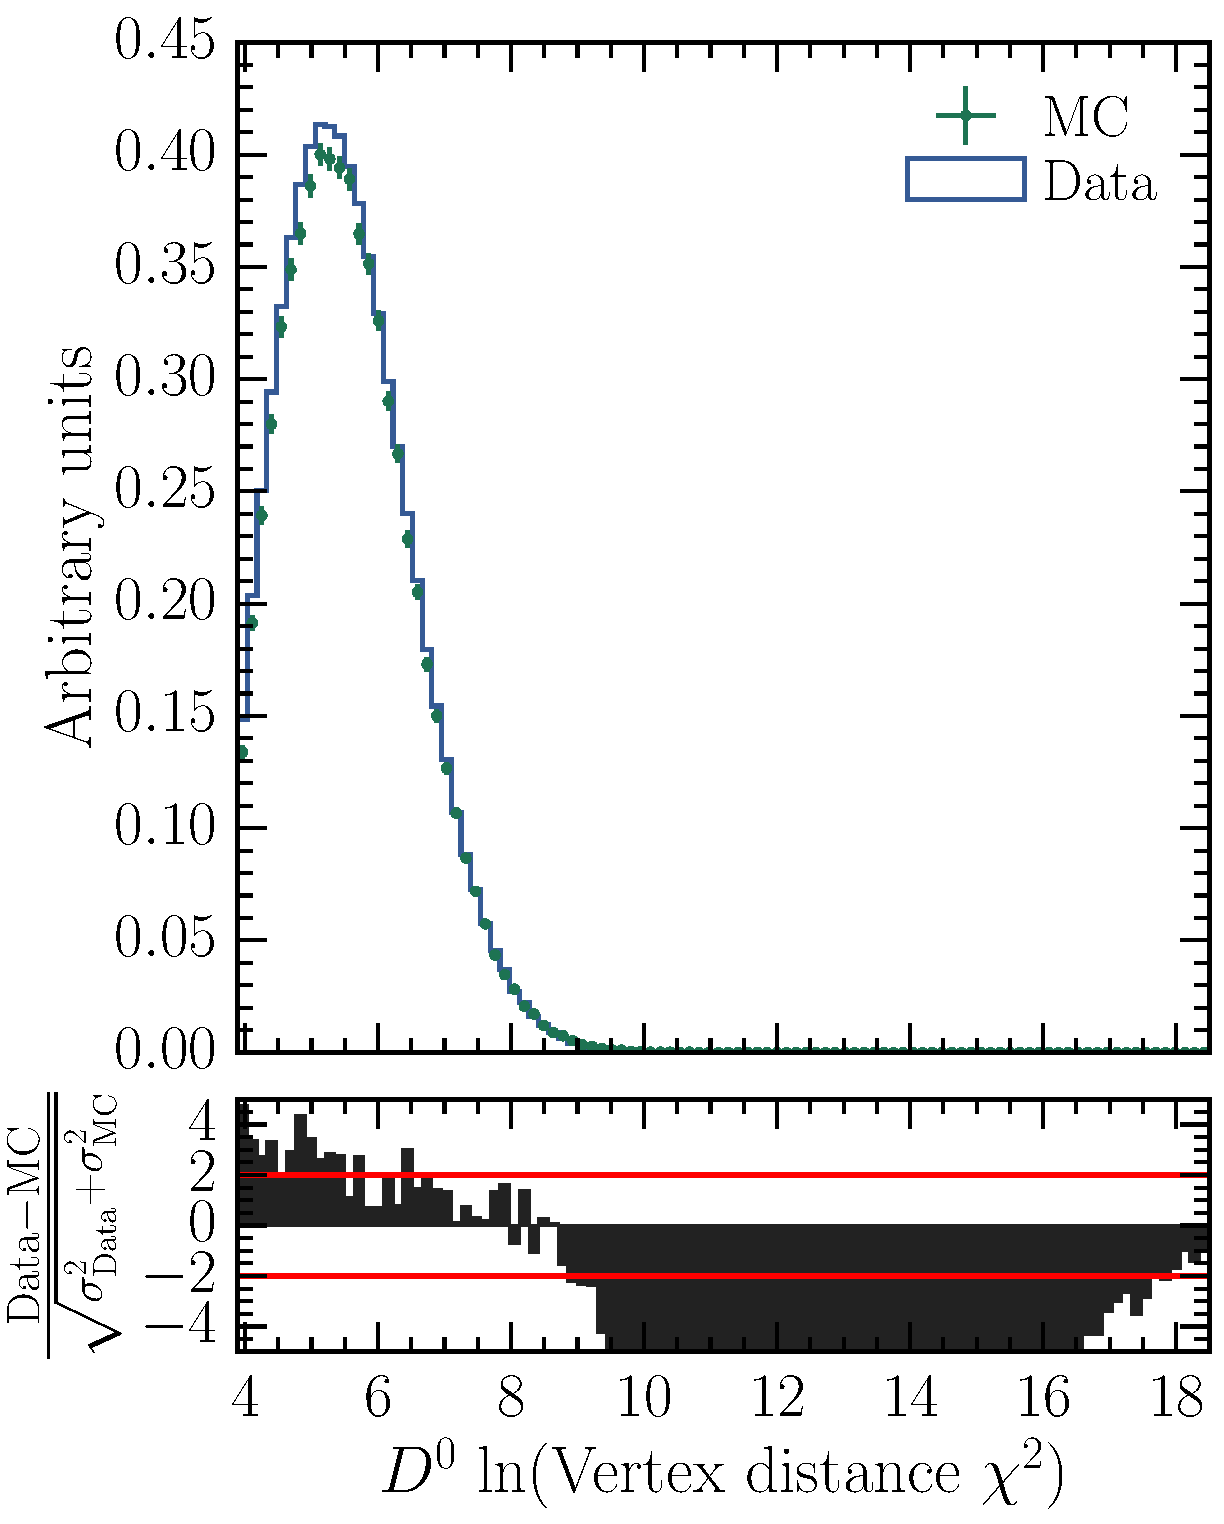
\includegraphics[width=\textwidth]{production/systematics/data_mc/D0_Loki_BPVVDCHI2}
    \caption{\PDzero VD \chisq}
  \end{subfigure}

  \begin{subfigure}{0.3\textwidth}
    \centering
    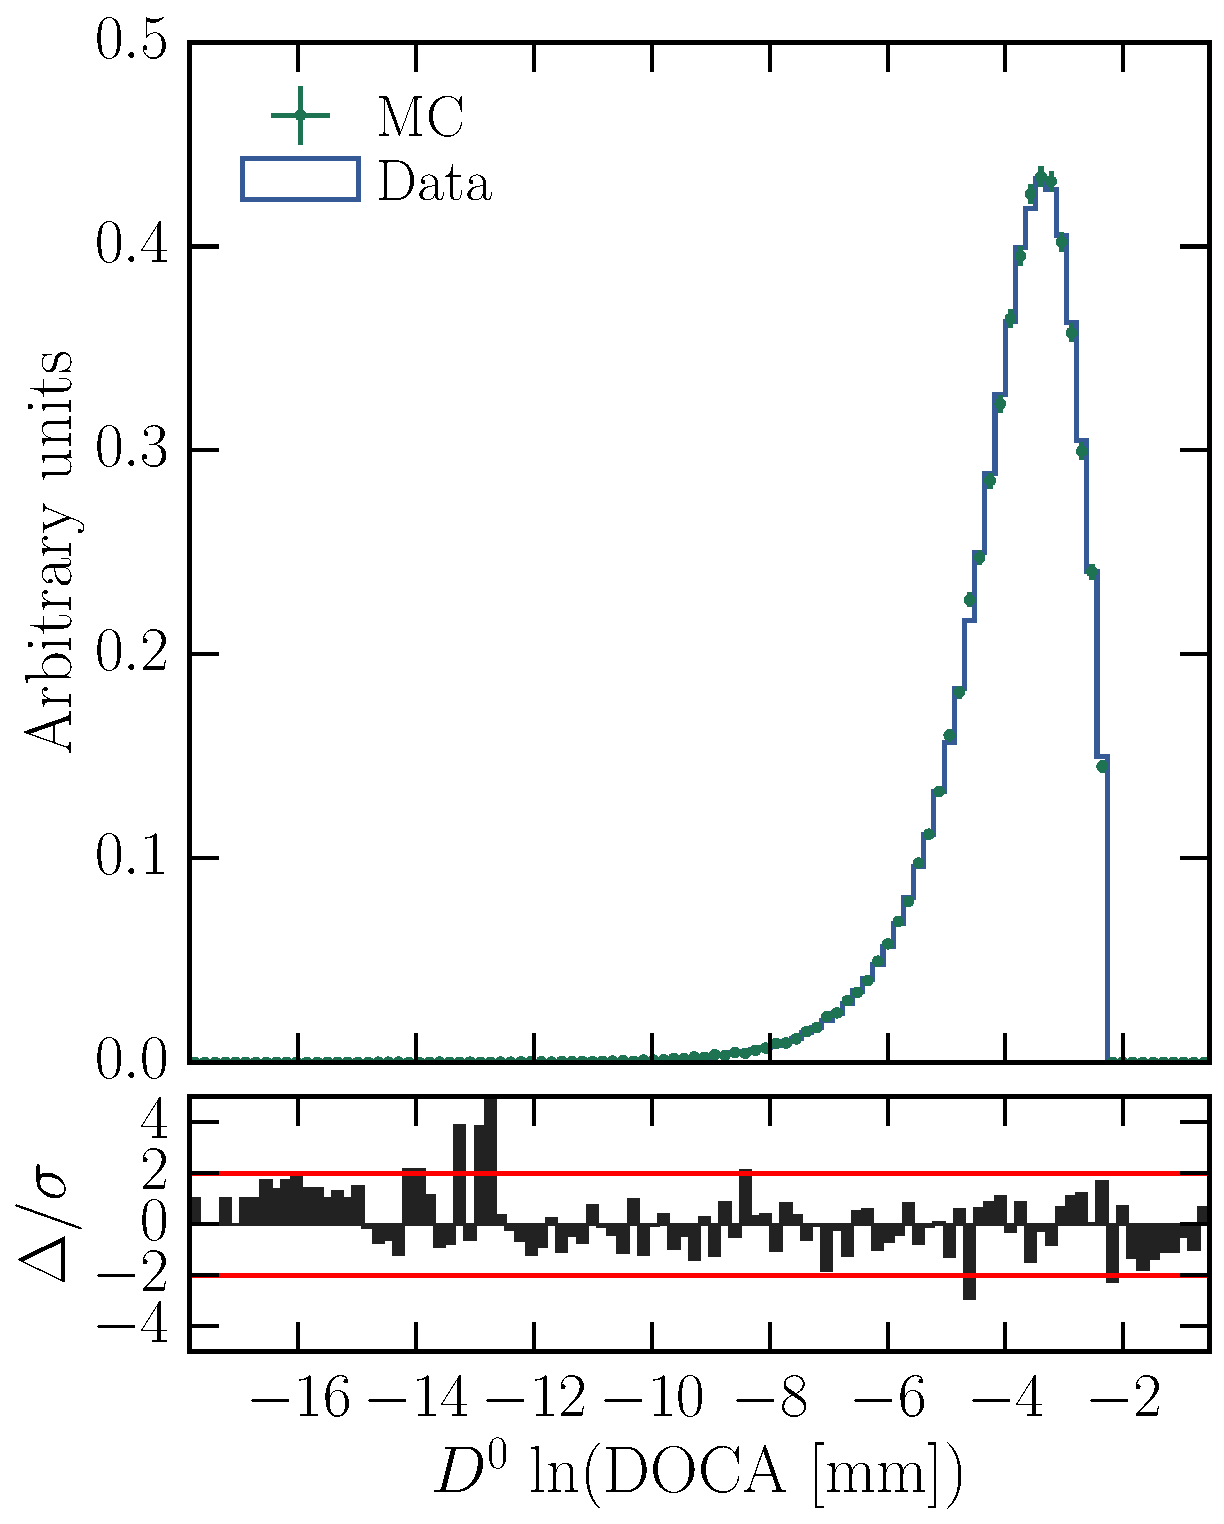
\includegraphics[width=\textwidth]{production/systematics/data_mc/D0_Loki_AMINDOCA}
    \caption{\PDzero \ac{DOCA}}
  \end{subfigure}
  \begin{subfigure}{0.3\textwidth}
    \centering
    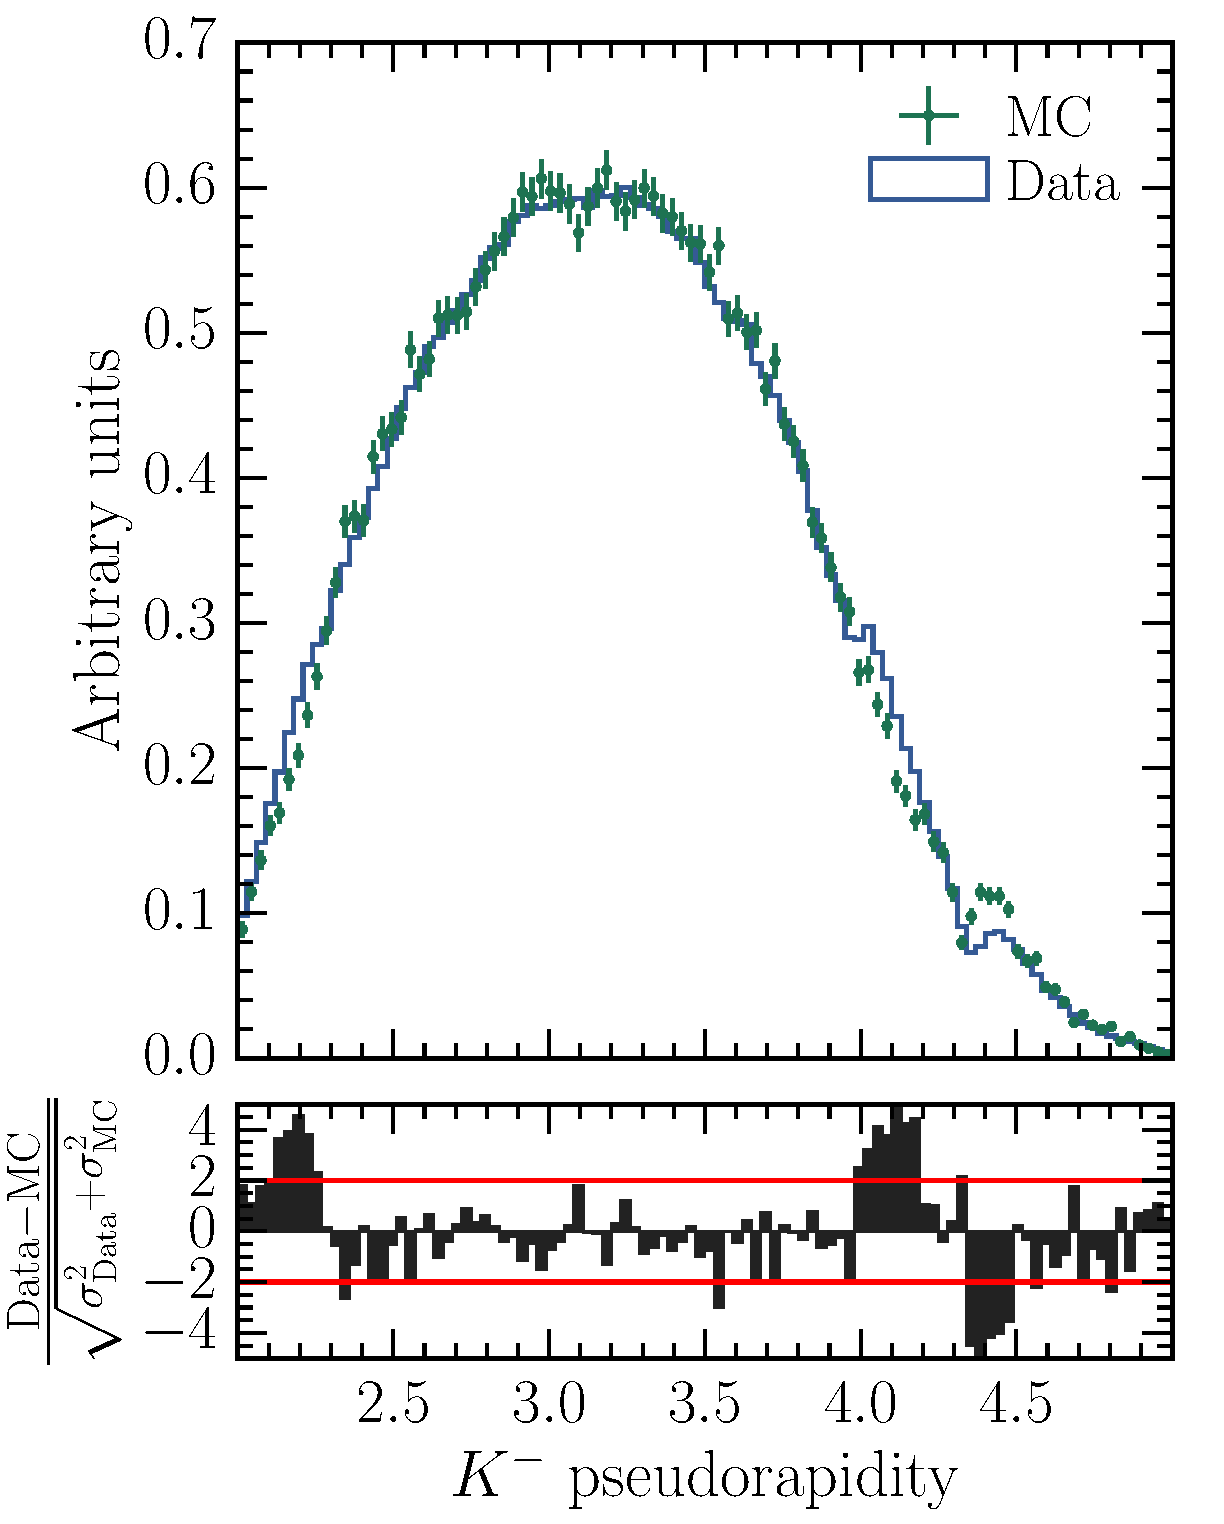
\includegraphics[width=\textwidth]{production/systematics/data_mc/D0_h1_ETA}
    \caption{Pion \Eta}
  \end{subfigure}
  \begin{subfigure}{0.3\textwidth}
    \centering
    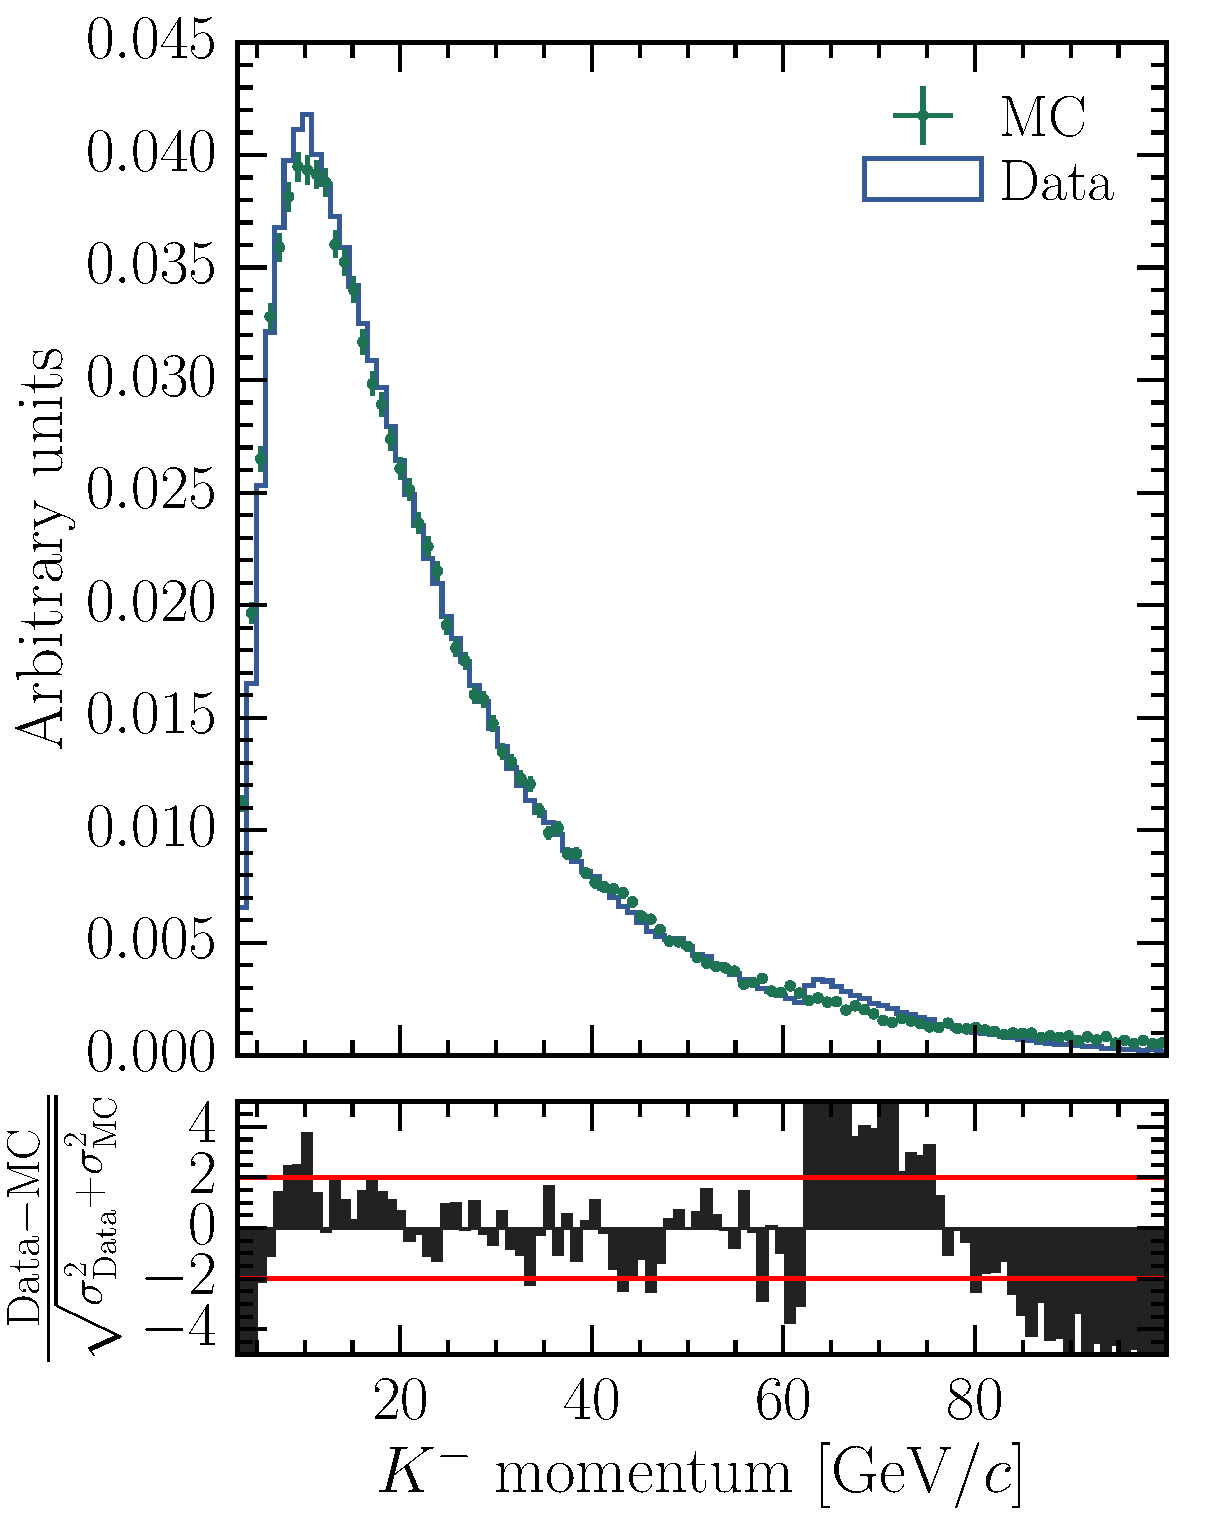
\includegraphics[width=\textwidth]{production/systematics/data_mc/D0_h1_P}
    \caption{Pion \ptot}
  \end{subfigure}

  \begin{subfigure}{0.3\textwidth}
    \centering
    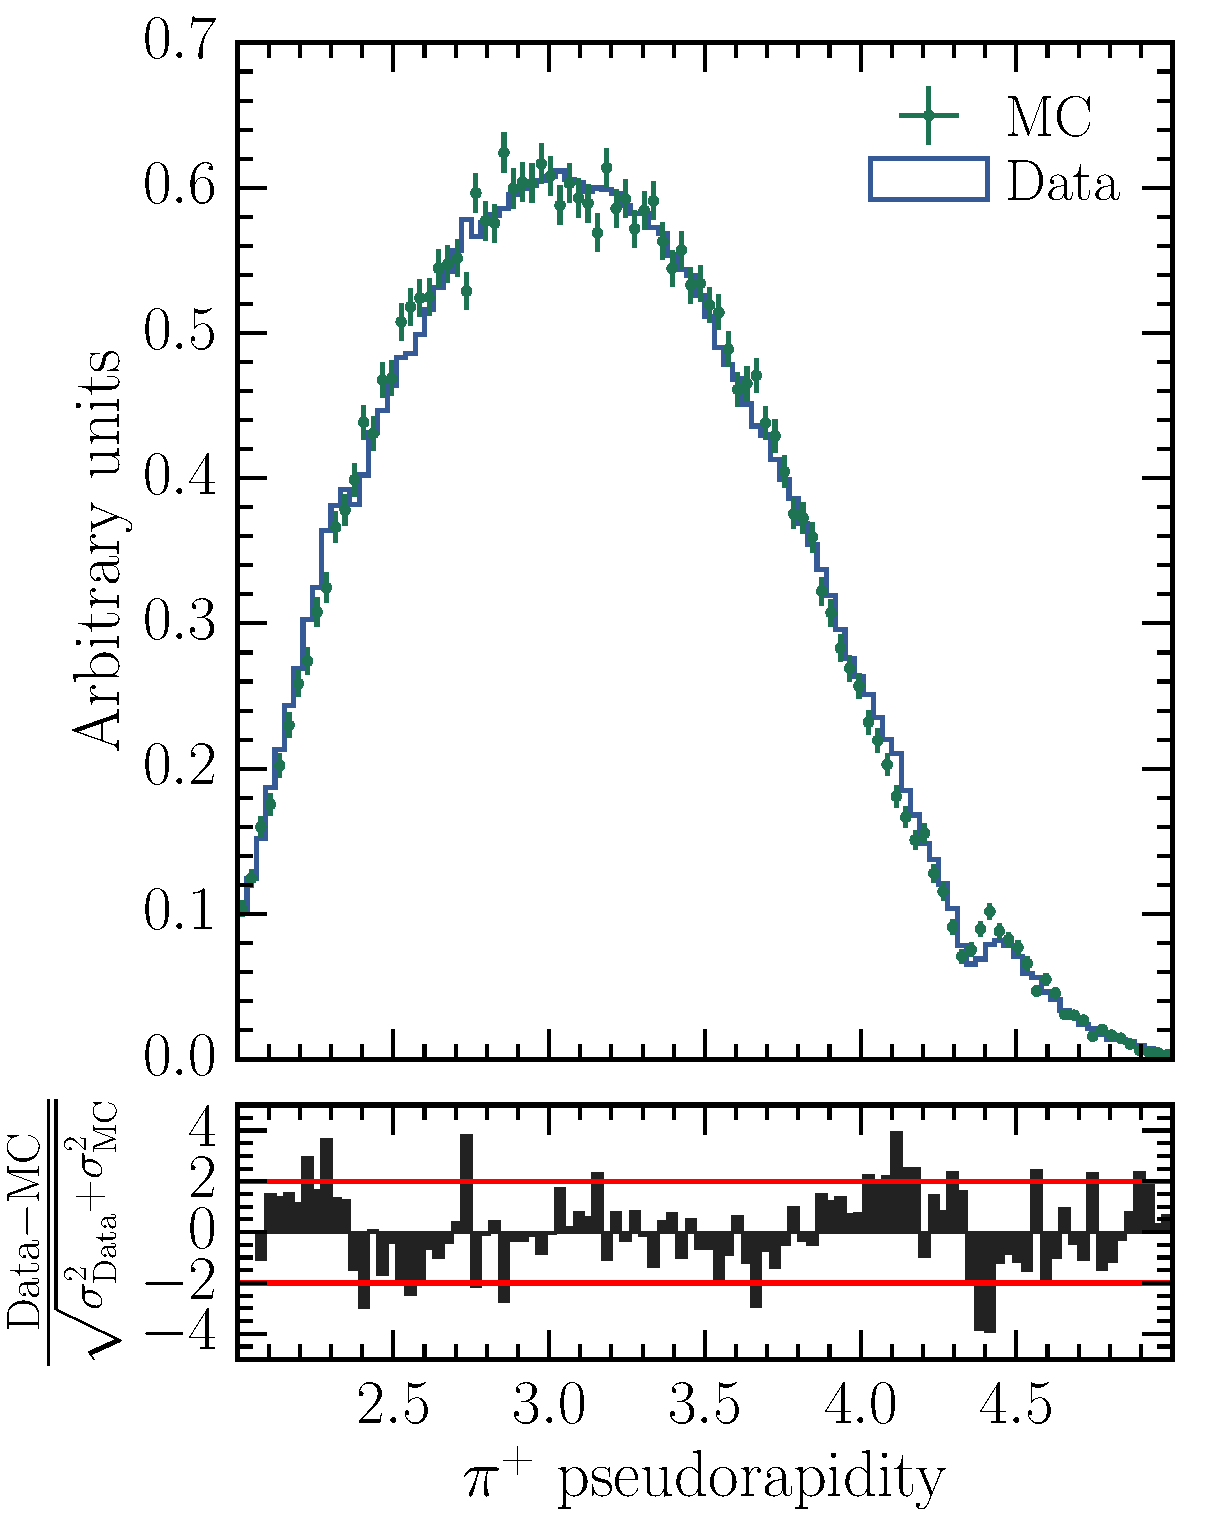
\includegraphics[width=\textwidth]{production/systematics/data_mc/D0_h2_ETA}
    \caption{Kaon \Eta}
  \end{subfigure}
  \begin{subfigure}{0.3\textwidth}
    \centering
    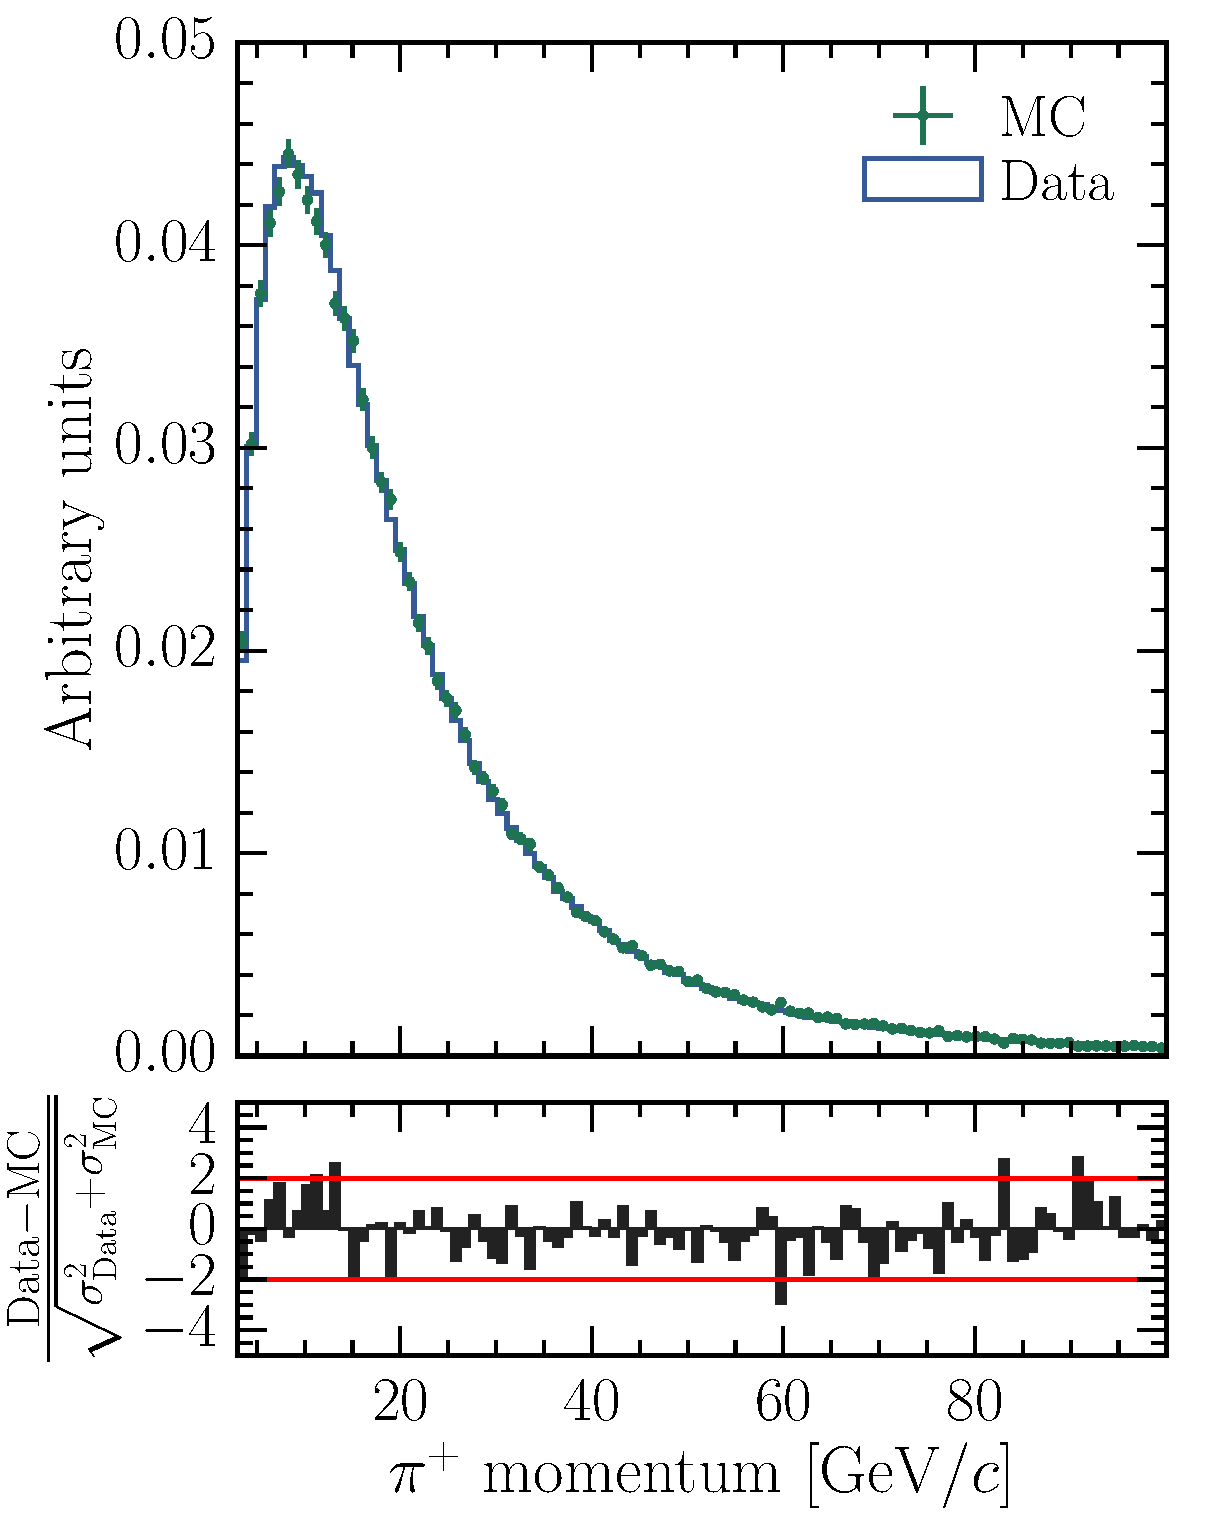
\includegraphics[width=\textwidth]{production/systematics/data_mc/D0_h2_P}
    \caption{Kaon \ptot}
  \end{subfigure}
  \begin{subfigure}{0.3\textwidth}
    \centering
    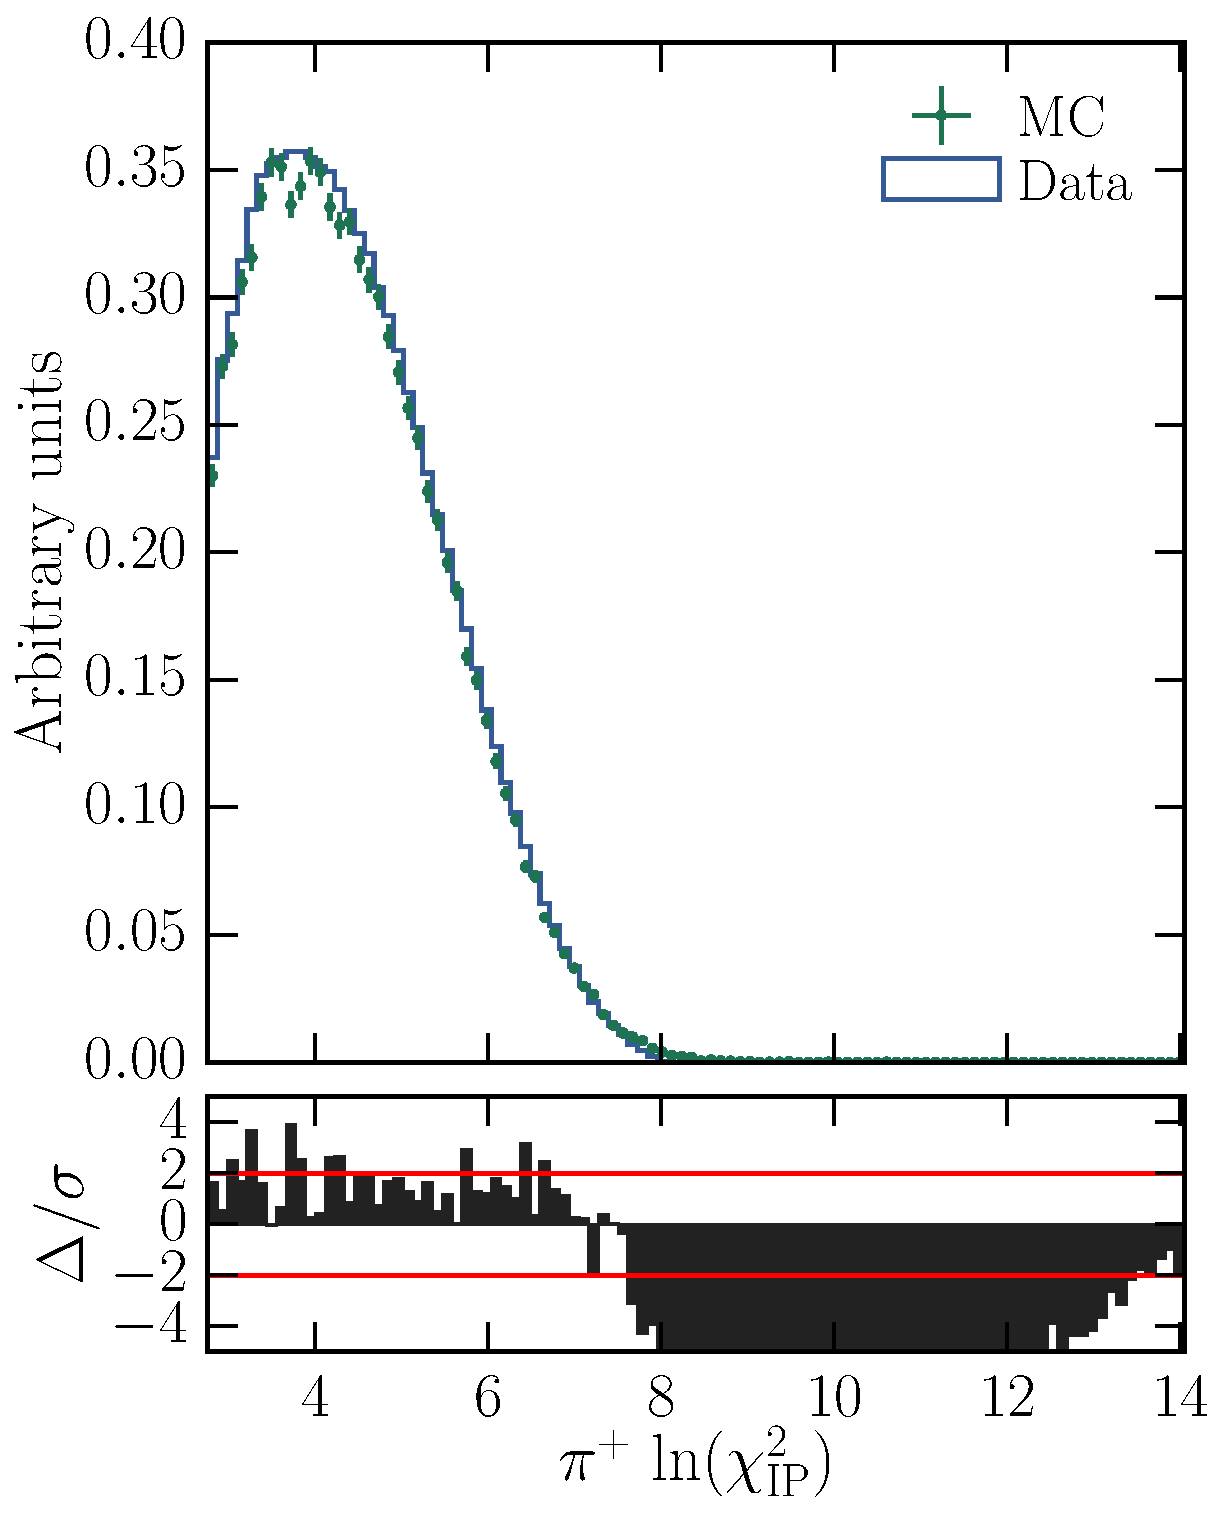
\includegraphics[width=\textwidth]{production/systematics/data_mc/D0_h2_Loki_MIPCHI2DV}
    \caption{Kaon \ipchisq}
  \end{subfigure}

  \caption{%
    Comparison of several variables used in the \DzToKpi selection between data 
    (blue line) and \ac{MC} (green points).
    Underneath each pair of distributions is a pull plot, showing the 
    significance of the deviation in each histogram bin.
  }
  \label{fig:prod:syst:mc:D0ToKpi}
\end{figure}

\begin{figure}
  \begin{subfigure}{0.3\textwidth}
    \centering
    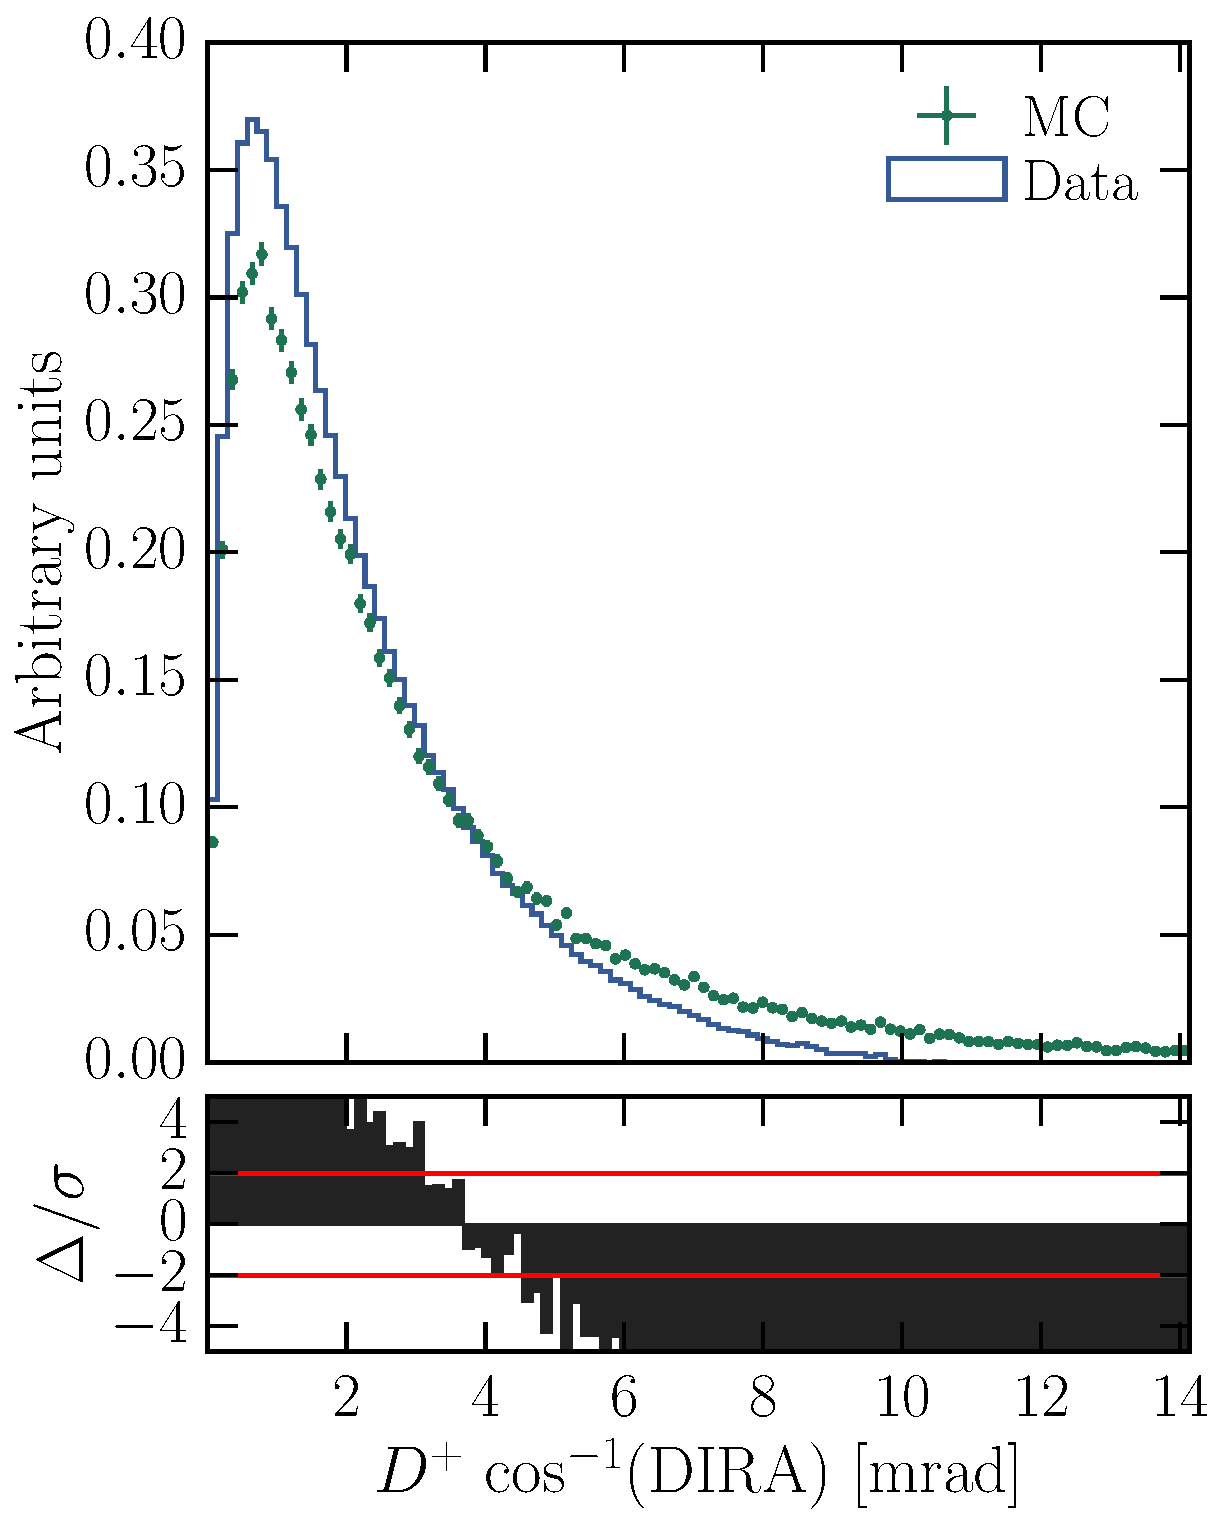
\includegraphics[width=\textwidth]{production/systematics/data_mc/Dp_DIRA_OWNPV}
    \caption{\PDplus \ac{DIRA}}
  \end{subfigure}
  \begin{subfigure}{0.3\textwidth}
    \centering
    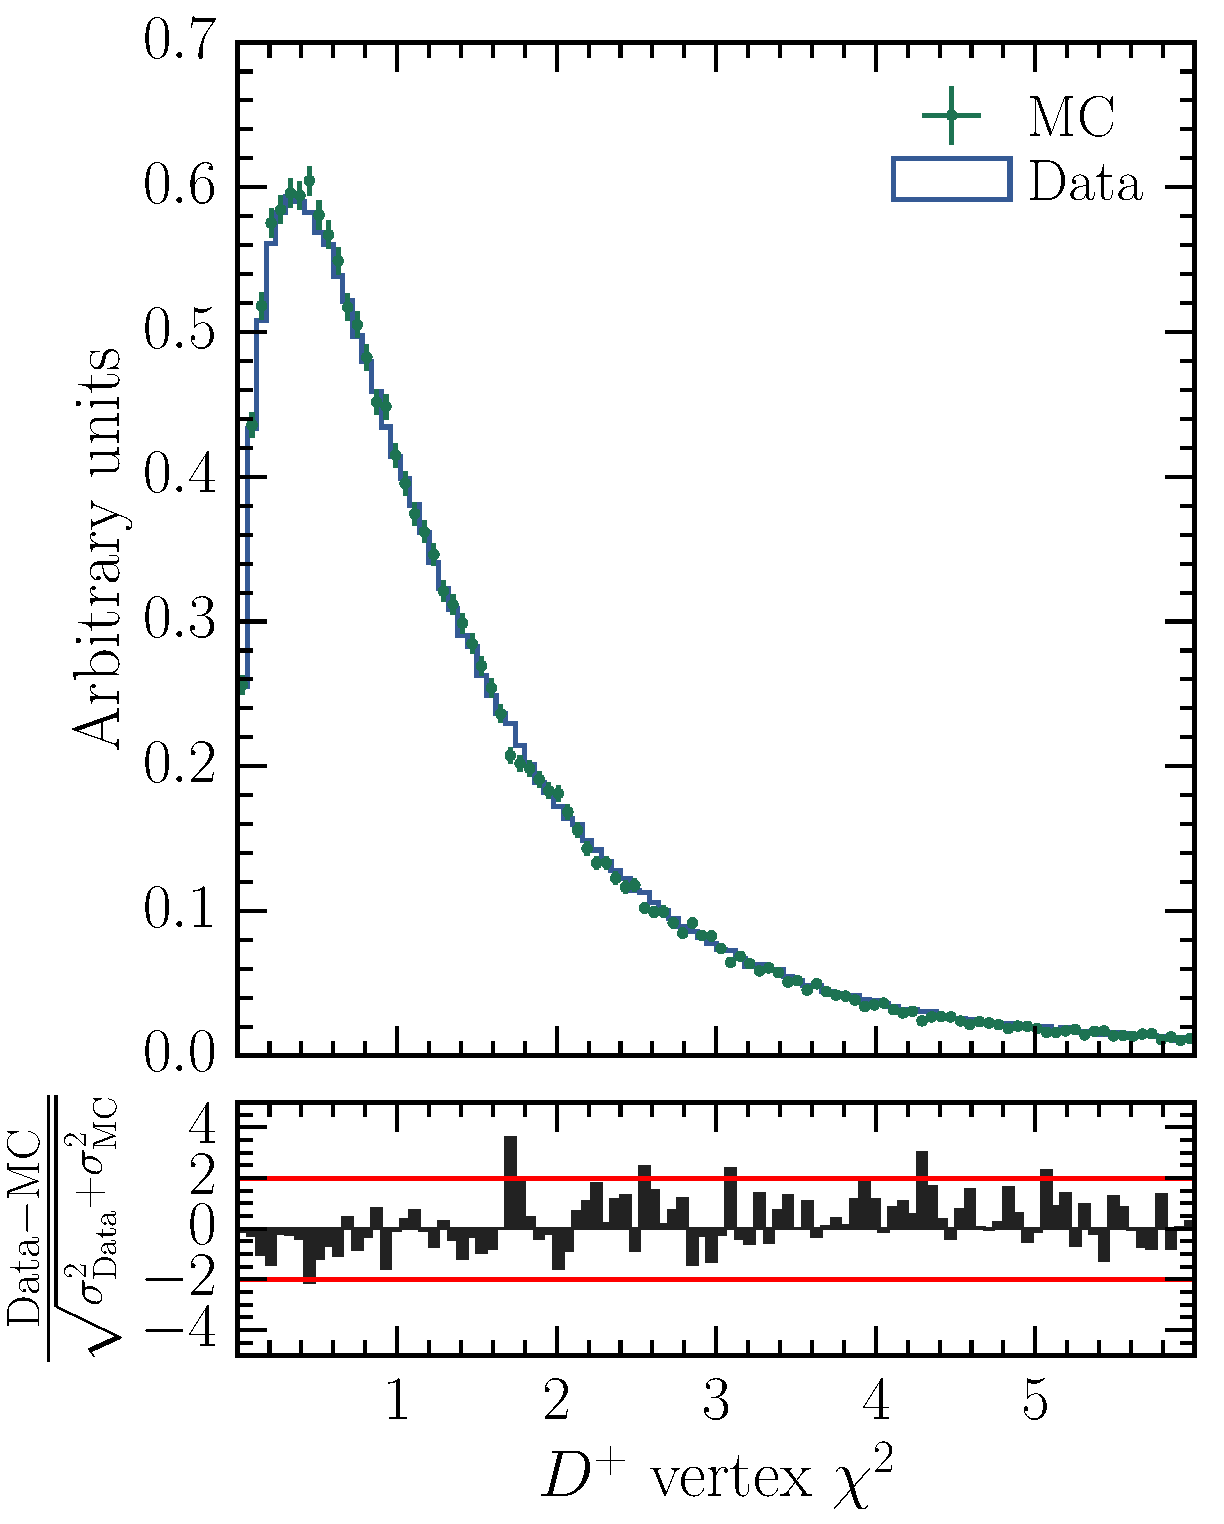
\includegraphics[width=\textwidth]{production/systematics/data_mc/Dp_ENDVERTEX_CHI2-Dp_ENDVERTEX_NDOF}
    \caption{\PDplus vertex \chisq}
  \end{subfigure}
  \begin{subfigure}{0.3\textwidth}
    \centering
    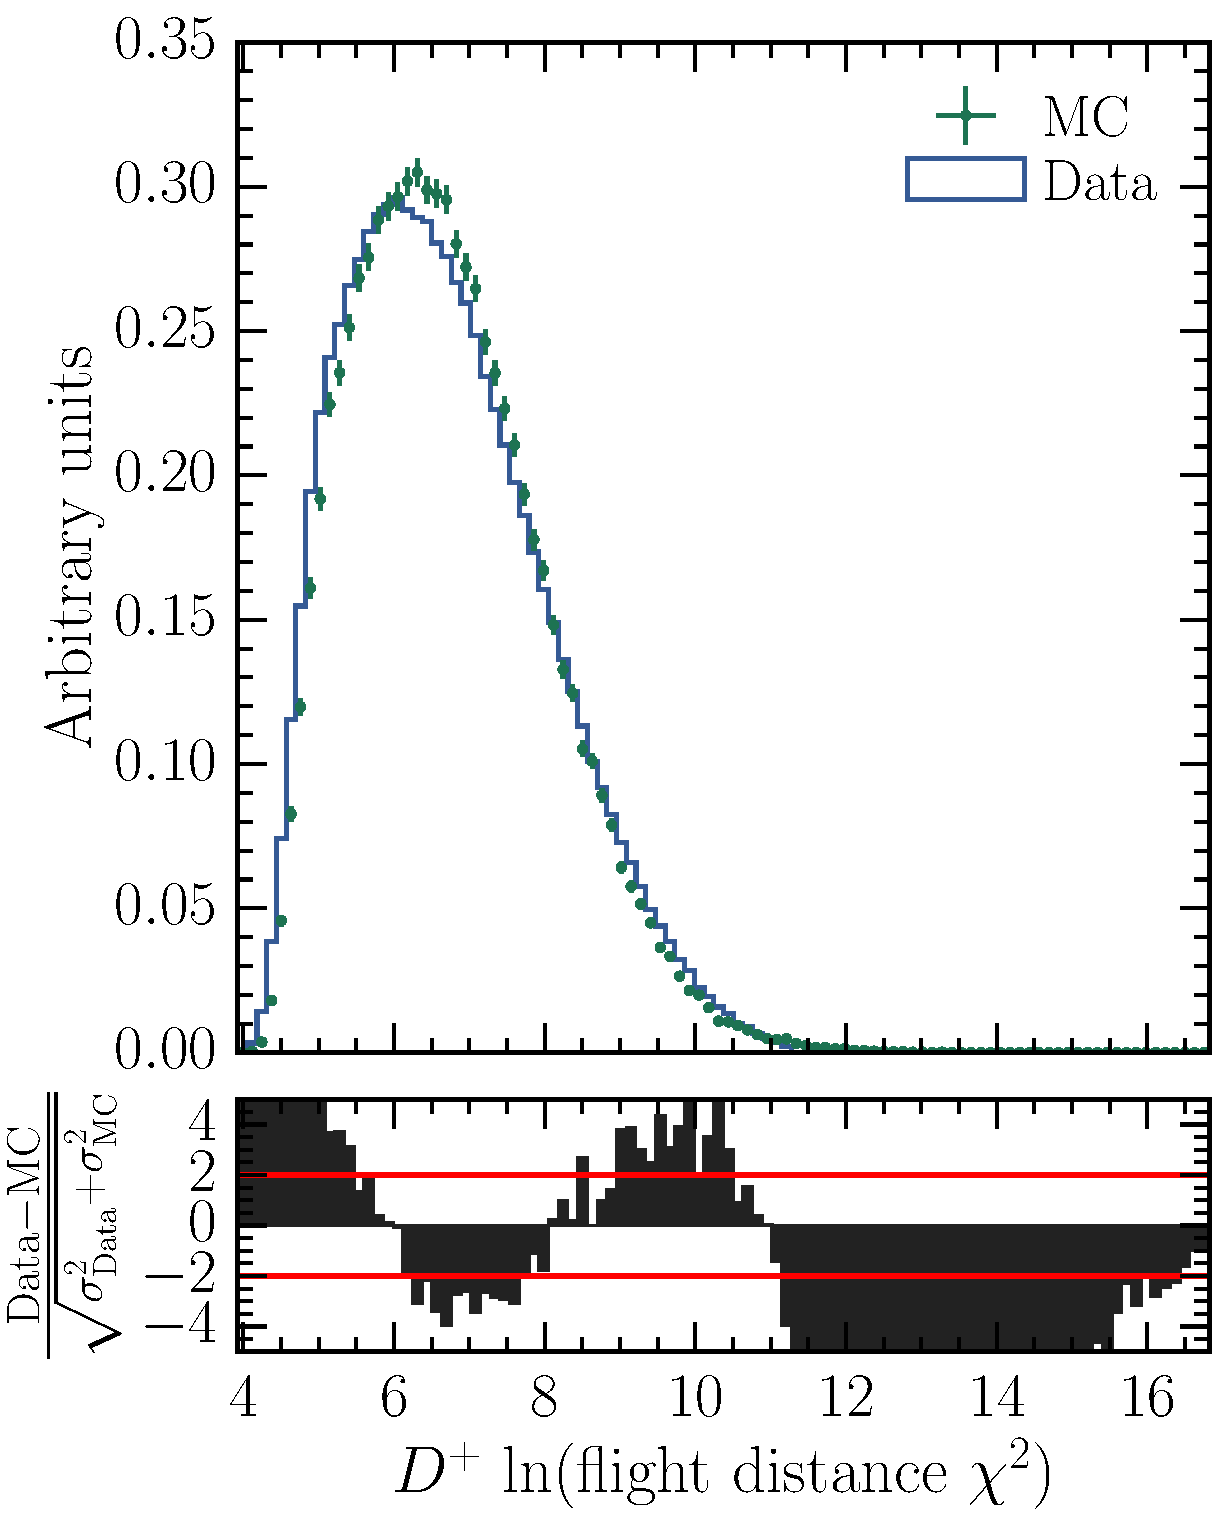
\includegraphics[width=\textwidth]{production/systematics/data_mc/Dp_FDCHI2_OWNPV}
    \caption{\PDzero FD \chisq}
  \end{subfigure}

  \begin{subfigure}{0.3\textwidth}
    \centering
    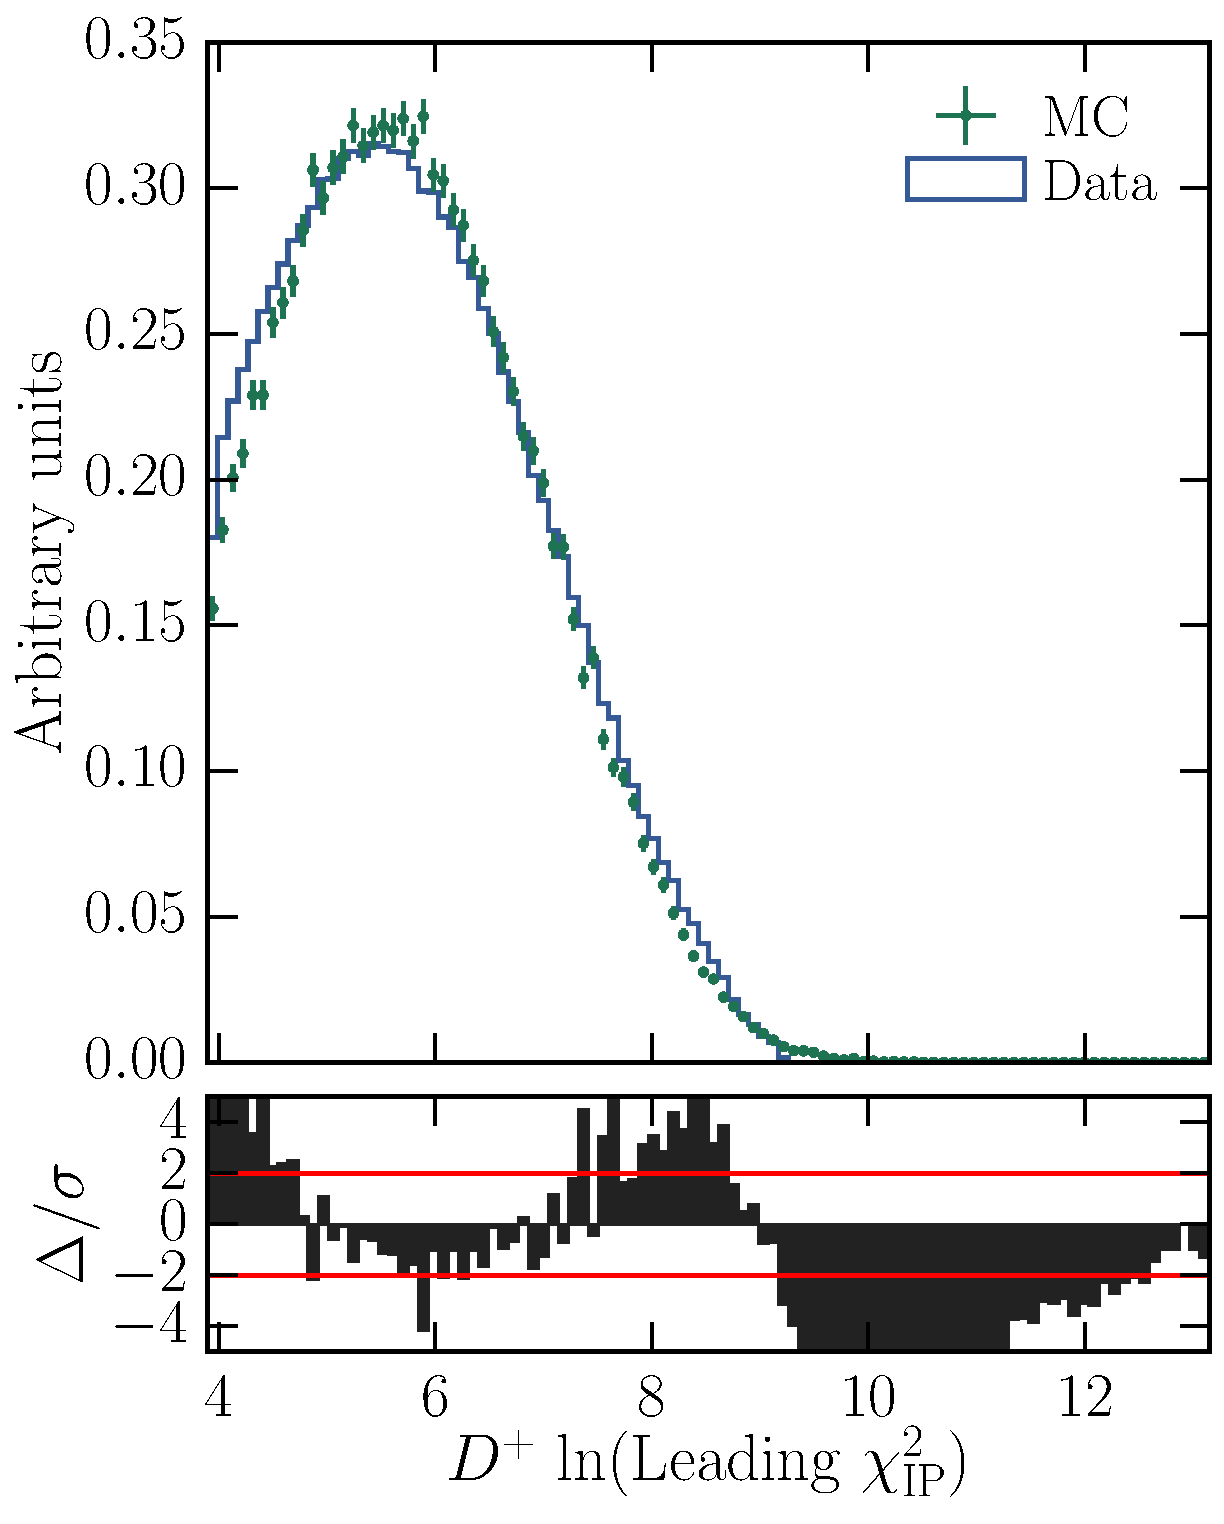
\includegraphics[width=\textwidth]{production/systematics/data_mc/Dp_Loki_MIPCHI2DV_First}
    \caption{Leading child \ipchisq}
  \end{subfigure}
  \begin{subfigure}{0.3\textwidth}
    \centering
    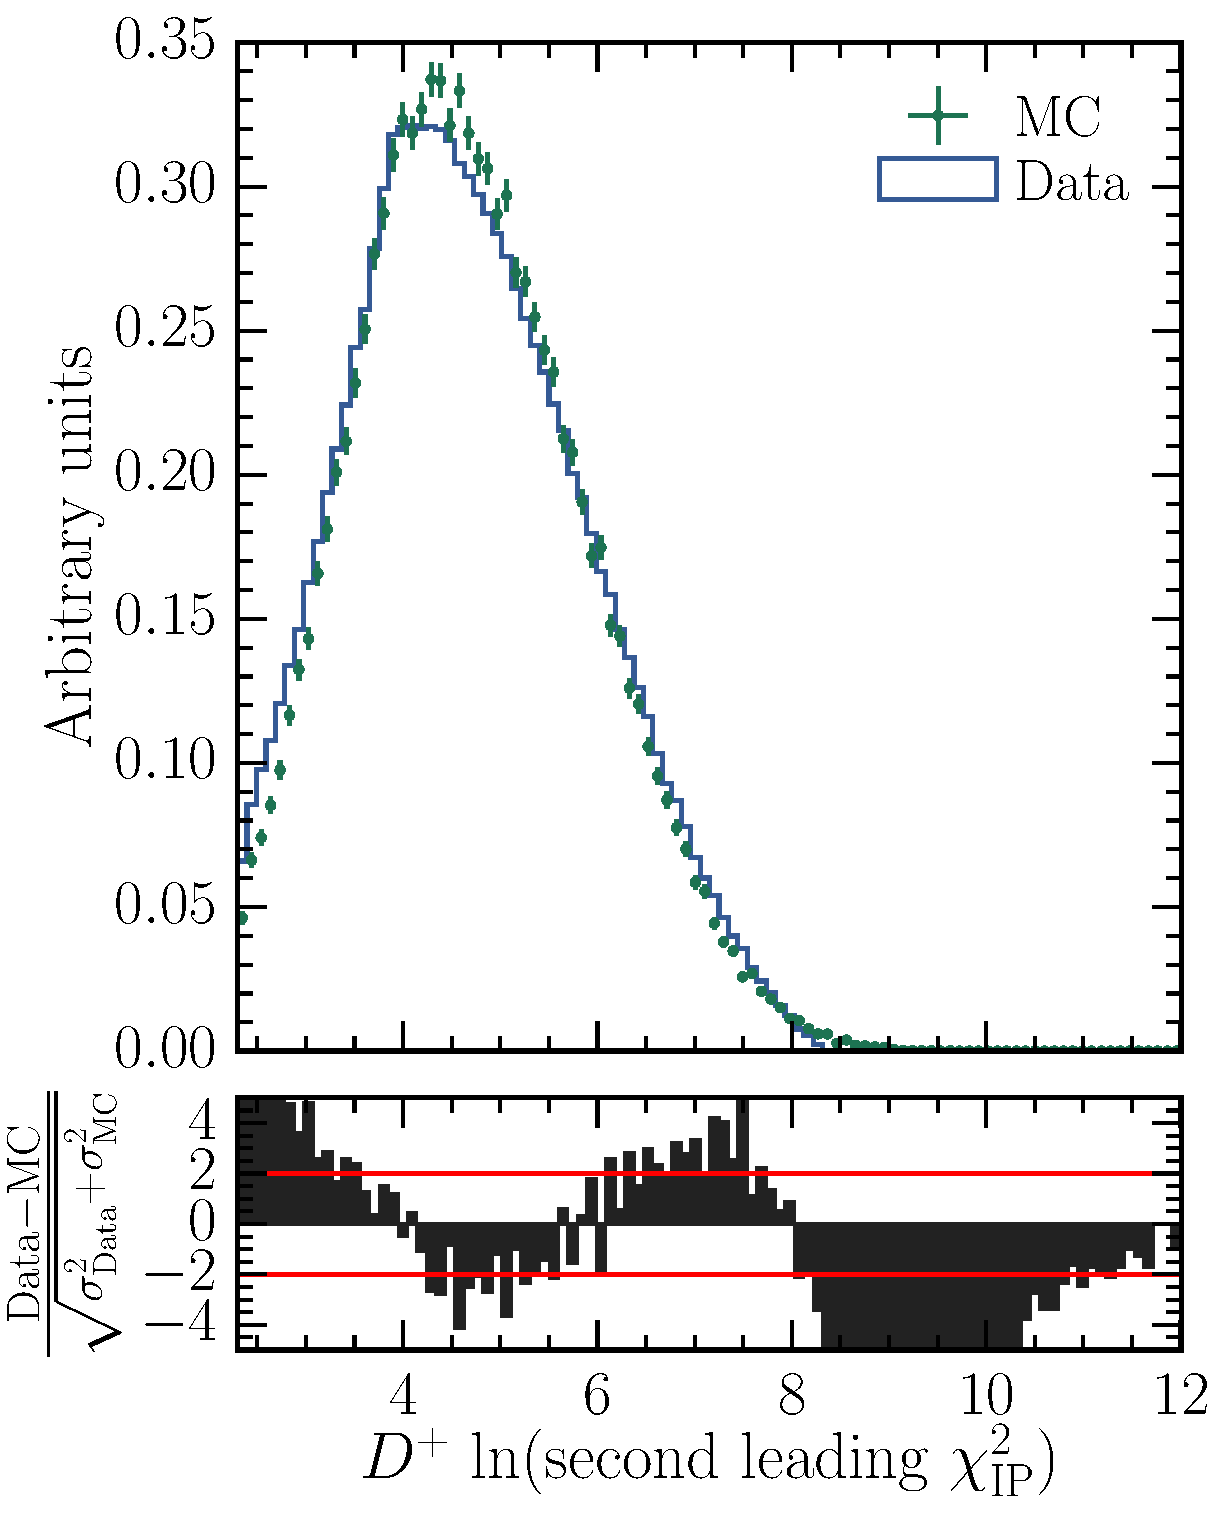
\includegraphics[width=\textwidth]{production/systematics/data_mc/Dp_Loki_MIPCHI2DV_Second}
    \caption{Second leading child \ipchisq}
  \end{subfigure}
  \begin{subfigure}{0.3\textwidth}
    \centering
    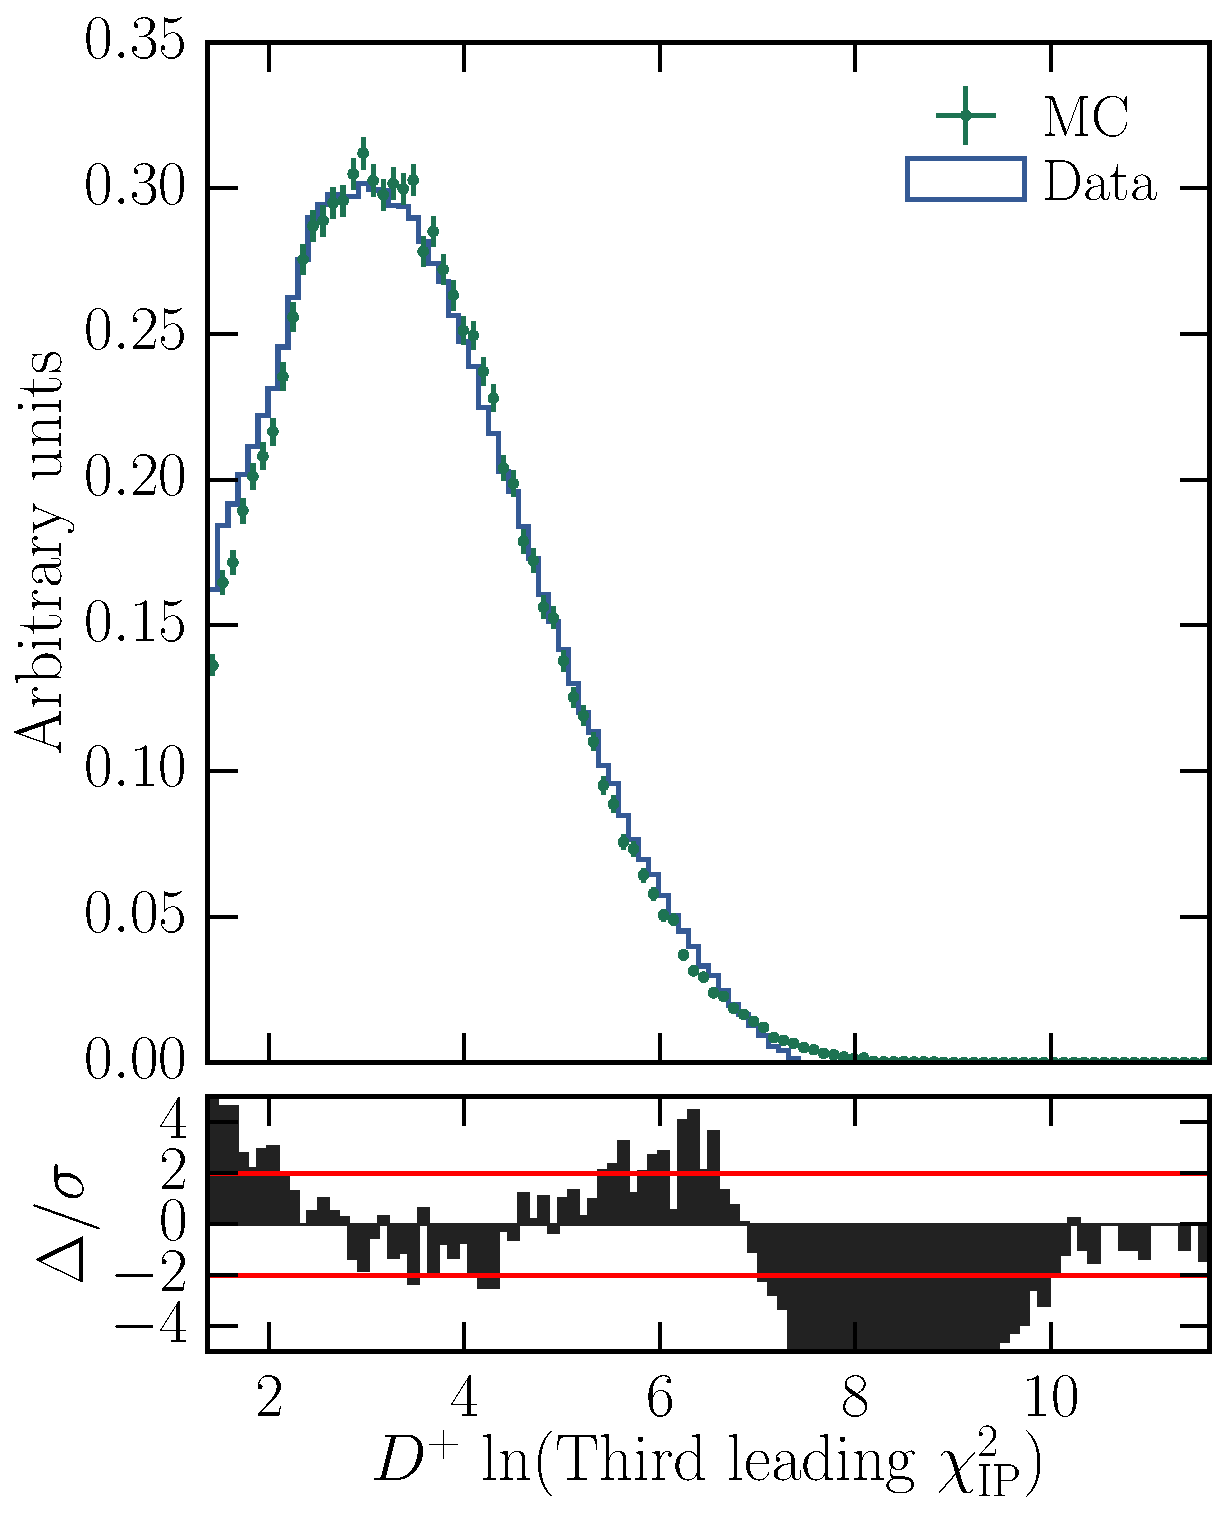
\includegraphics[width=\textwidth]{production/systematics/data_mc/Dp_Loki_MIPCHI2DV_Third}
    \caption{Third leading child \ipchisq}
  \end{subfigure}

  \begin{subfigure}{0.3\textwidth}
    \centering
    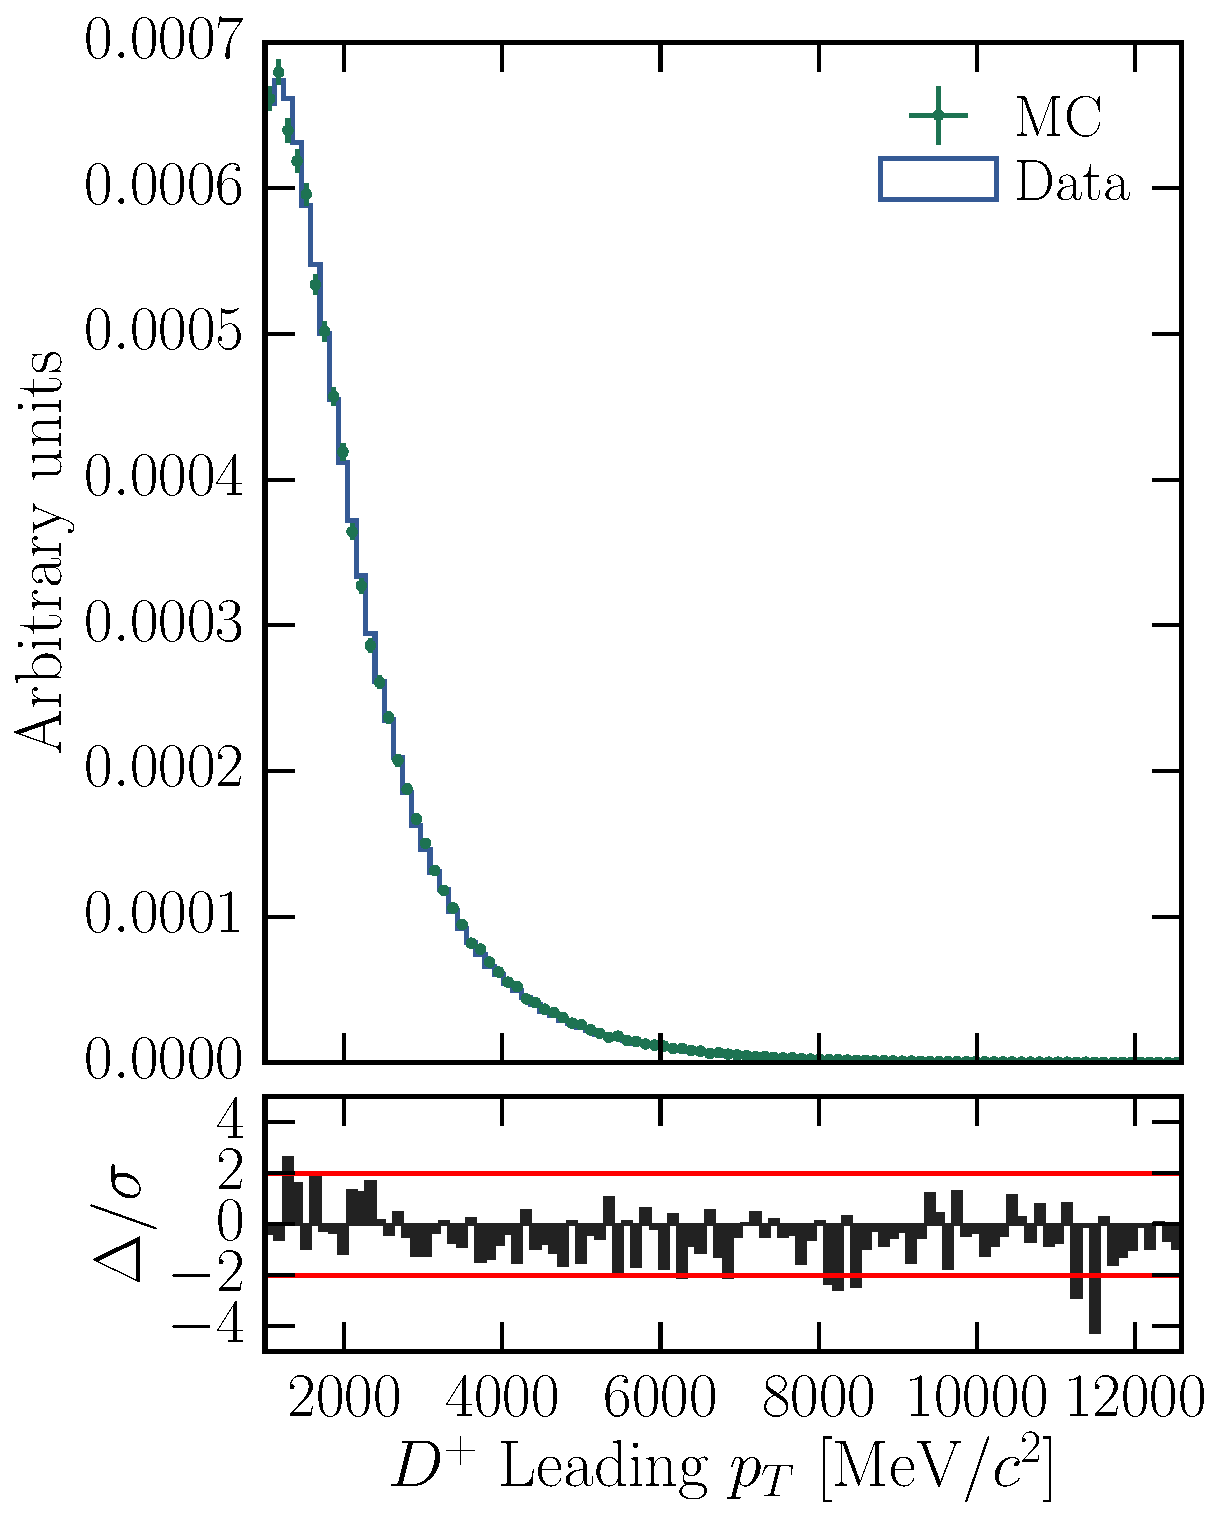
\includegraphics[width=\textwidth]{production/systematics/data_mc/Dp_PT_First}
    \caption{Leading child \pT}
  \end{subfigure}
  \begin{subfigure}{0.3\textwidth}
    \centering
    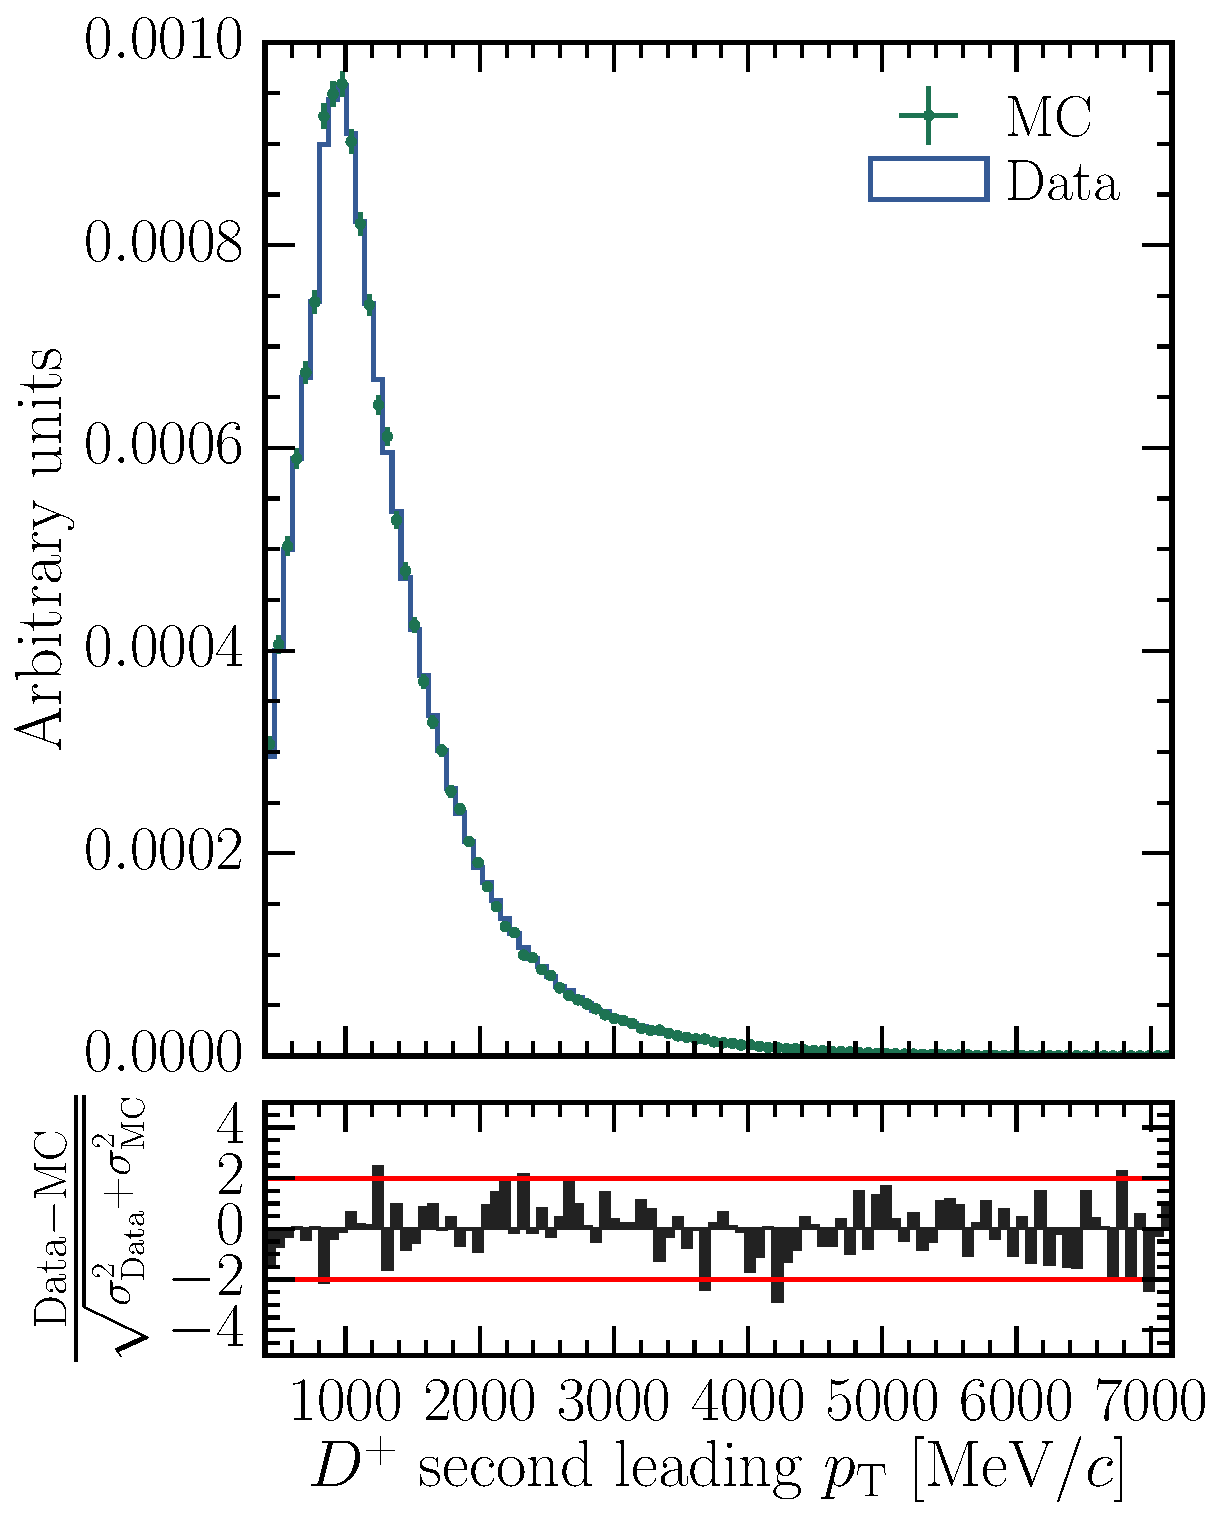
\includegraphics[width=\textwidth]{production/systematics/data_mc/Dp_PT_Second}
    \caption{Second leading child \pT}
  \end{subfigure}
  \begin{subfigure}{0.3\textwidth}
    \centering
    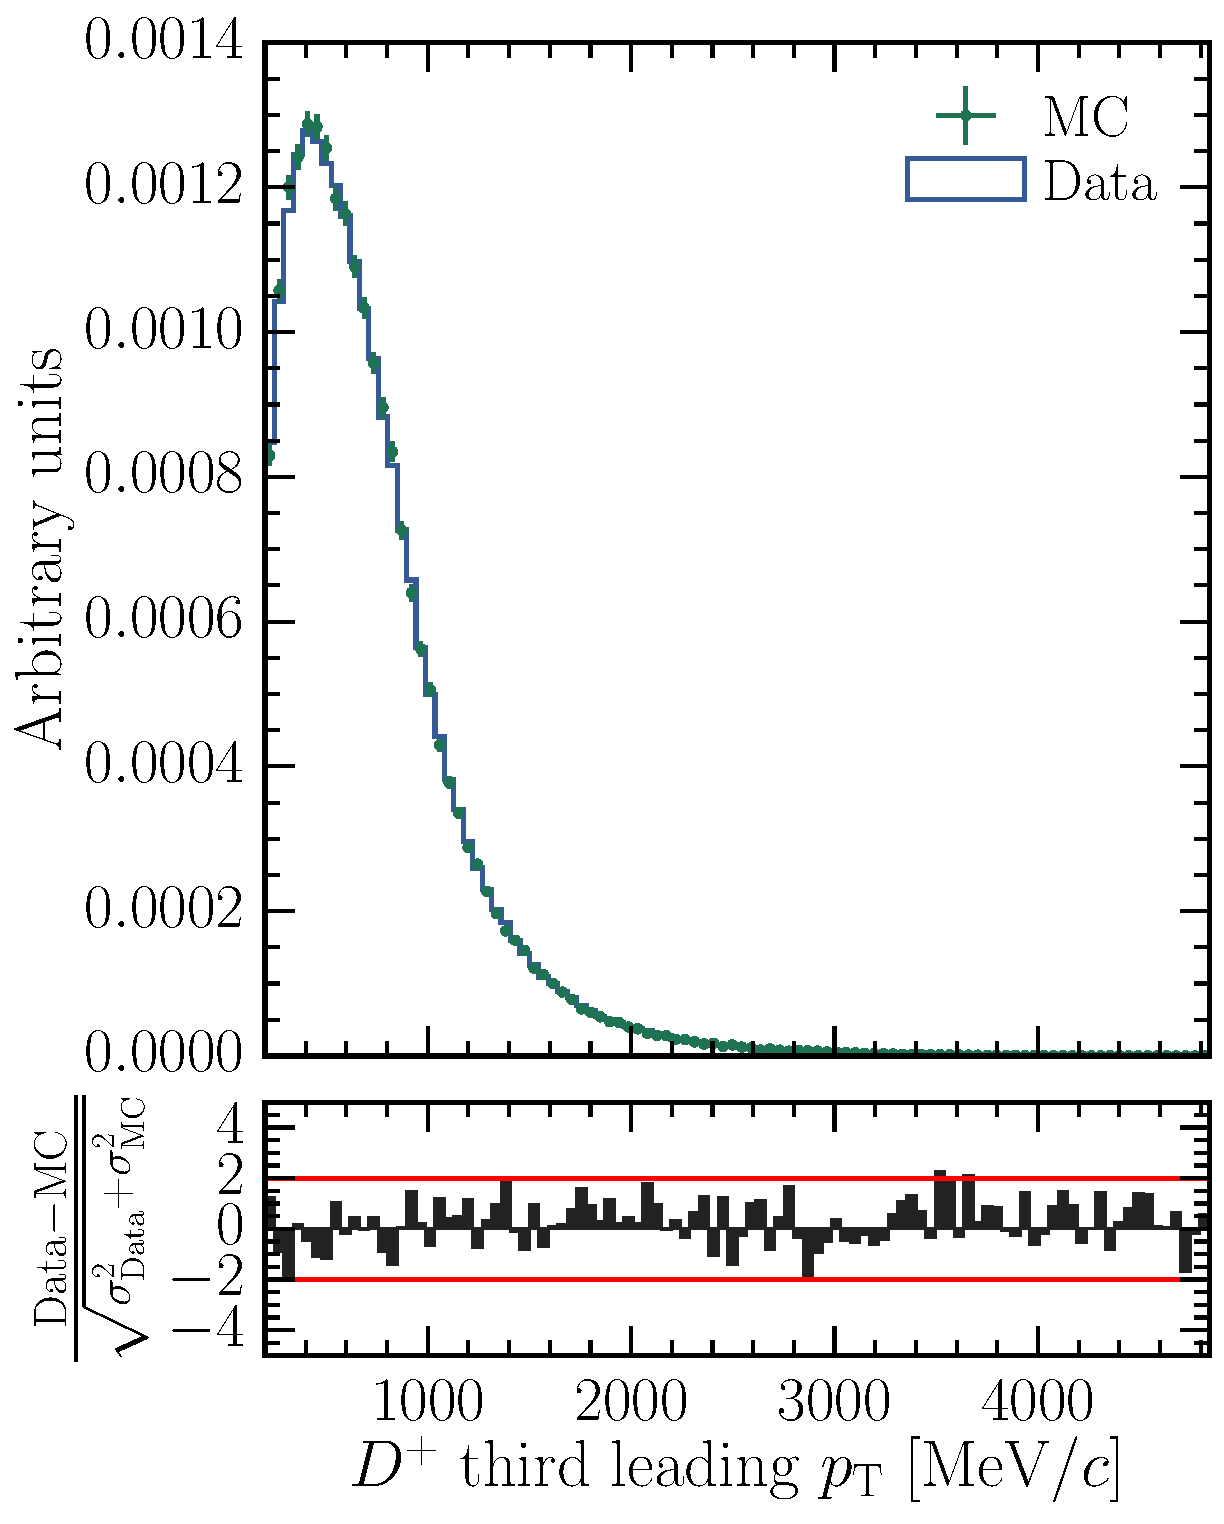
\includegraphics[width=\textwidth]{production/systematics/data_mc/Dp_PT_Third}
    \caption{Third leading child \pT}
  \end{subfigure}

  \caption{%
    Comparison of several variables used in the \DpToKpipi selection between 
    data (blue line) and \ac{MC} (green points).
    Underneath each pair of distributions is a pull plot, showing the 
    significance of the deviation in each histogram bin.
  }
  \label{fig:prod:syst:mc:DpToKpipi}
\end{figure}

\section{Monte Carlo truth matching}
\label{chap:prod:syst:mc:truth_matching}

The truth matching efficiency described in \cref{chap:prod:effs:truth} is computed using an \ac{MC} 
sample of finite size, and so carries a statistical uncertainty.
As in \cref{chap:prod::syst:mcstat}, this statistical uncertainty is propagated to the cross-section 
measurements as a systematic uncertainty.
Unlike the selection efficiency uncertainty, the \ac{MC} sample size is too 
small to compute the truth matching systematic in \pTy\ bins, and so an 
integrated value is computed.
The values for each mode are given in Table~\ref{tab:prod:syst:mc:truth_matching}.

\section{Particle identification calibration}
\label{chap:prod:syst:pid}

As stated in \cref{chap:prod:effs:pid}, a key assumption in the \ac{PID} 
calibration is that the \ac{PID} efficiency \effpid\ is single-valued in a 
\ptotetanspd\ bin.
Generally, this assumption is satisfied by an infinitely fine binning, but the 
limited statistics of the calibration sample prohibit this as it would create 
large statistical uncertainties.
There are two systematic uncertainties associated to this effect: the 
statistical uncertainty on \effpid\ due to the finite size of the calibration 
sample; and the breakdown of the assumption that \effpid\ is single-valued in a 
\ptotetanspd\ bin.

\subsection{Calibration sample size}
\label{chap:prod:syst:pid:stat}

The efficiency \effi\ in the $i$th \ptotetanspd\ bin of the efficiency 
histogram has a statistical uncertainty $\unc{\effi}$ due to the finite size of 
the calibration sample.
Each \ptotetanspd\ bin contains a disjoint set of calibration tracks, and hence 
the efficiencies between bins fluctuate independently, hence there will be a 
non-zero correlation between the \ac{PID} efficiencies of tracks in a single 
decay if those tracks fall in the same efficiency bin, as well as between 
different decays if there is an overlap in the efficiency bins that are used.
To model these correlations, a series of ten thousand pseudo-experiments are 
performed to propagate the statistical uncertainty on \effi\ to a corresponding 
uncertainty on \effpid.

In each pseudo-experiment, a new set of efficiencies $\effi'$ is drawn from a 
normal distribution of mean \effi\ and width $\unc{\effi}$.
The full calibration procedure is then repeated using the set of $\effi'$ to 
obtain an overall efficiency $\effpid'$ for that pseudo-experiment.
The statistical uncertainty $\unc_{C}{\effpid}$ on the nominal efficiency is 
then taken to be the standard deviation of the distribution of $\effpid'$.

A common set of efficiency histograms is generated and is used in all 
pseudo-experiments for computing the uncertainty in each bin for all charm 
mesons, allowing the correlations to be determined.
As different \pTy\ bins and decay modes have different kinematic distributions 
for their final state particles, this correlation is found to be significant 
within a decay mode only for neighbouring \pTy\ bins, and negligible between 
different modes.

The relative uncertainty $\unc_{C}{\effpid}/\effpid$ is given in 
\cref{tab:syst:pid:binning:D0ToKpi,tab:syst:pid:binning:DpToKpipi} for 
\DzToKpi\ and \DpToKpipi.
The distribution in $\effpid'$ is taken as the posterior \ac{PDF} for this 
uncertainty in the \ac{MC} error propagation, translated such that the most 
probable value is coincident with zero.

\subsection{Binning scheme}
\label{chap:prod:syst:pid:binning}

The iterative procedure to find the binning scheme used for the efficiency 
histograms, described in \cref{chap:prod:effs:pid:binning}, is limited by the 
sample size of the calibration data.
To be able to assess the possible shift in \effpid\ one would see if the 
calibration sample size was larger, two-dimensional \acp{PDF} in track \ptot\ 
and \Eta\ are made using \acp{KDE}~\cite{Poluektov:2014rxa}.
The event multiplicity is not modelled as the \ac{PID} efficiency variation in 
this feature is seen to be significantly smaller than that in track \ptot\ and 
\Eta, and hence \effpid\ is less sensitive to the binning in that variable.

One two-dimensional \ac{KDE} is constructed for each particle species both 
before and after the \ac{PID} requirements under study.
These densities $P_{\PK/\Ppi}(\ptot, \Eta)$ and $P'_{\PK/\Ppi}(\ptot, \Eta)$
can be used to obtain the efficiency \effi\ in the $(\ptot,\,\Eta)$ bin of 
volume $V$ as
\begin{equation}
  \effi = \frac{C'}{C}\frac{%
    \int_{V} P'(\ptot,\Eta)\dif{p}\dif{\Eta}
  }{%
    \int_{V} P(\ptot,\Eta)\dif{p}\dif{\Eta}
  },
\end{equation}
where $C(')$ is the total signal calibration sample size before (after) the 
requirements.
\Cref{fig:prod:syst:pid:kde_eta} shows example one-dimensional \ac{KDE} 
projections in kaon \Eta\ in various \ptot\ bins in comparison with the signal 
calibration data.
\Cref{fig:prod:syst:pid:kde_1d_binning} shows the one-dimensional projections 
of the efficiencies in comparison with a fine one-dimensional binned 
approximation.
In both cases, a good agreement is seen between the \ac{KDE} estimate and the 
data.

The \acp{KDE} are used as generative \acp{PDF} to produce pseudo-experimental 
data with which to perform the \ac{PID} calibration.
\Cref{fig:prod:syst:pid:kde_2d_binning:kaon,fig:prod:syst:pid:kde_2d_binning:pion} 
compare the two-dimensional efficiency histogram from the real calibration data 
and the nominal binning with that generated from the \acp{KDE}, and a good 
agreement is seen between the two.
Unlike with real calibration data, an effectively infinite amount of data can 
be generated from the \acp{KDE}, allowing the effects of the binning scheme to 
be probed.
This is done by computing \effpid\ with a progressively finer binning until the 
value converges, as shown in \cref{fig:prod:syst:pid:convergence}.
The difference $\unc_{B}{\effpid}$ between the value at convergence and that 
found in the nominal procedure is taken as the systematic uncertainty on 
\effpid\ due to the chosen binning.
A normal distribution is assumed for the corresponding nuisance parameter.
The same convergence behaviour is seen in all \pTy\ bins and across all modes, 
are so the uncertainty is assumed to be fully correlated across them.

The systematic uncertainty due to the choice of \ptotetanspd\ binning relative 
to the measured cross-section value is given in 
\cref{tab:syst:pid:binning:D0ToKpi,tab:syst:pid:binning:DpToKpipi} for 
\DzToKpi\ and \DpToKpipi.

\begin{figure}
  \begin{subfigure}{0.5\textwidth}
    \centering
    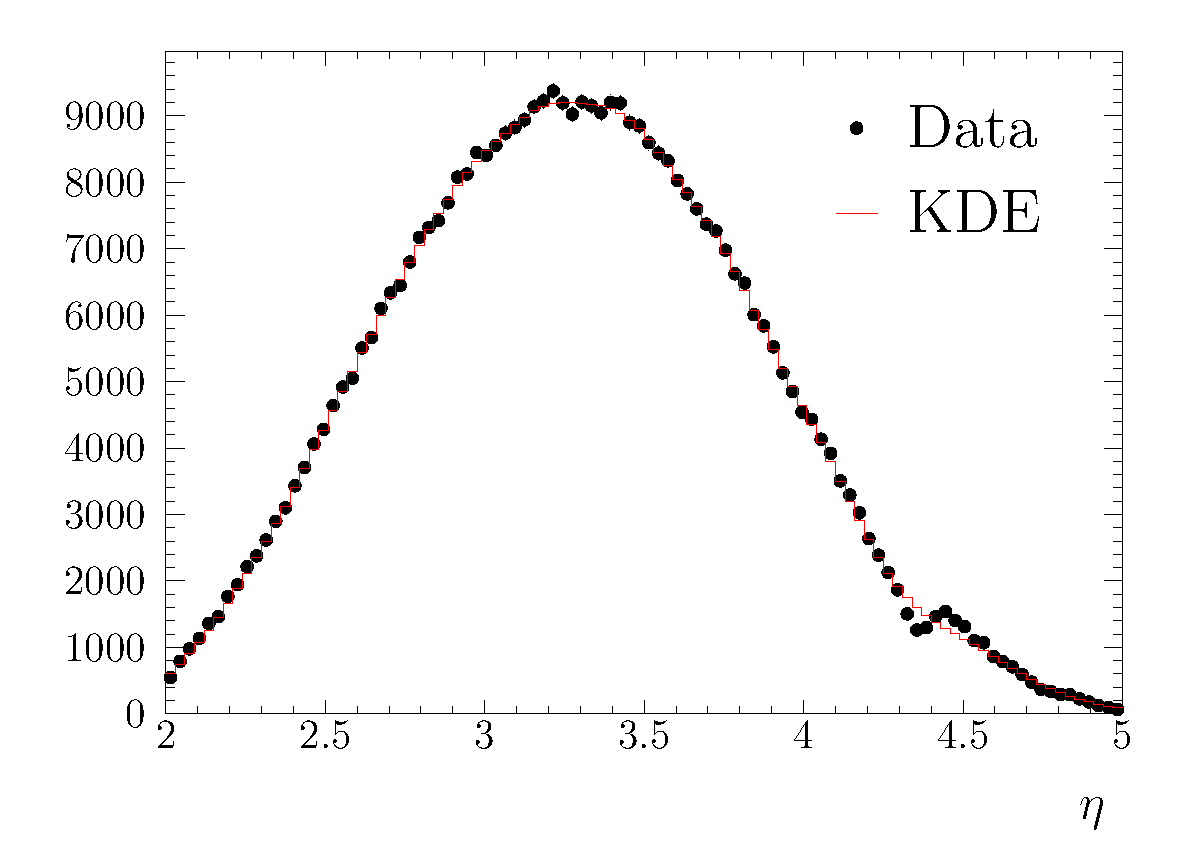
\includegraphics[width=\textwidth]{production/systematics/PIDK_binning_eta_integrated}
    \caption{\ptotrange{3}{100}}
    \label{fig:prod:syst:pid:kde_eta:integrated}
  \end{subfigure}
  \begin{subfigure}{0.5\textwidth}
    \centering
    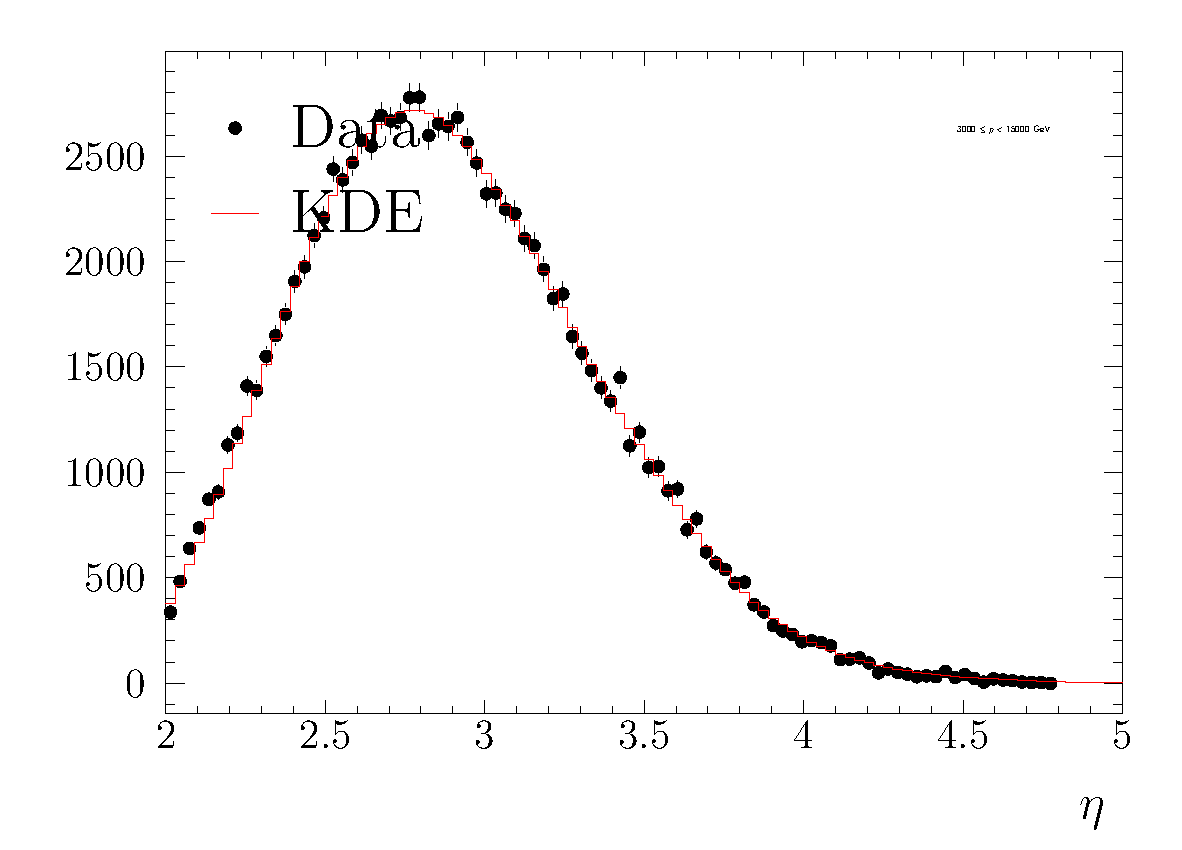
\includegraphics[width=\textwidth]{production/systematics/PIDK_binning_eta_bin1}
    \caption{\ptotrange{3}{15}}
    \label{fig:prod:syst:pid:kde_eta:bin1}
  \end{subfigure}
  \begin{subfigure}{0.5\textwidth}
    \centering
    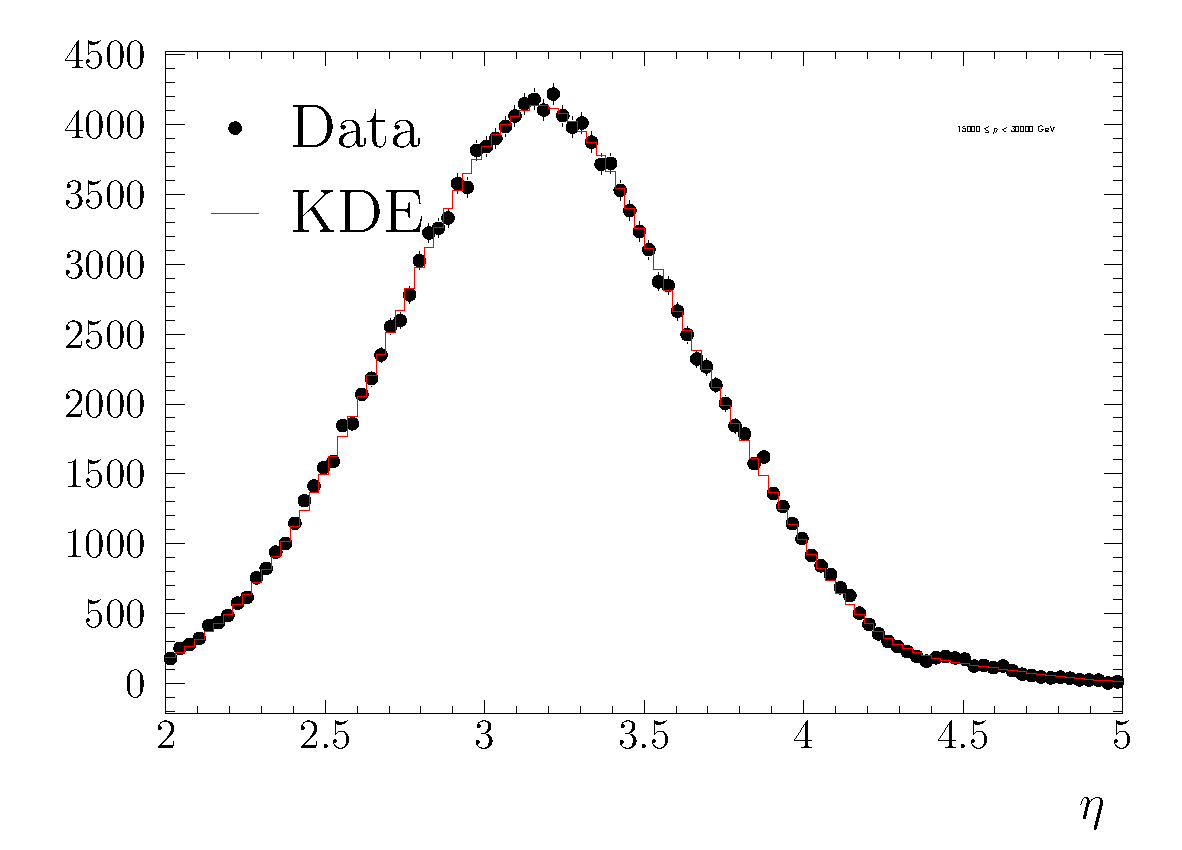
\includegraphics[width=\textwidth]{production/systematics/PIDK_binning_eta_bin2}
    \caption{\ptotrange{15}{30}}
    \label{fig:prod:syst:pid:kde_eta:bin2}
  \end{subfigure}
  \begin{subfigure}{0.5\textwidth}
    \centering
    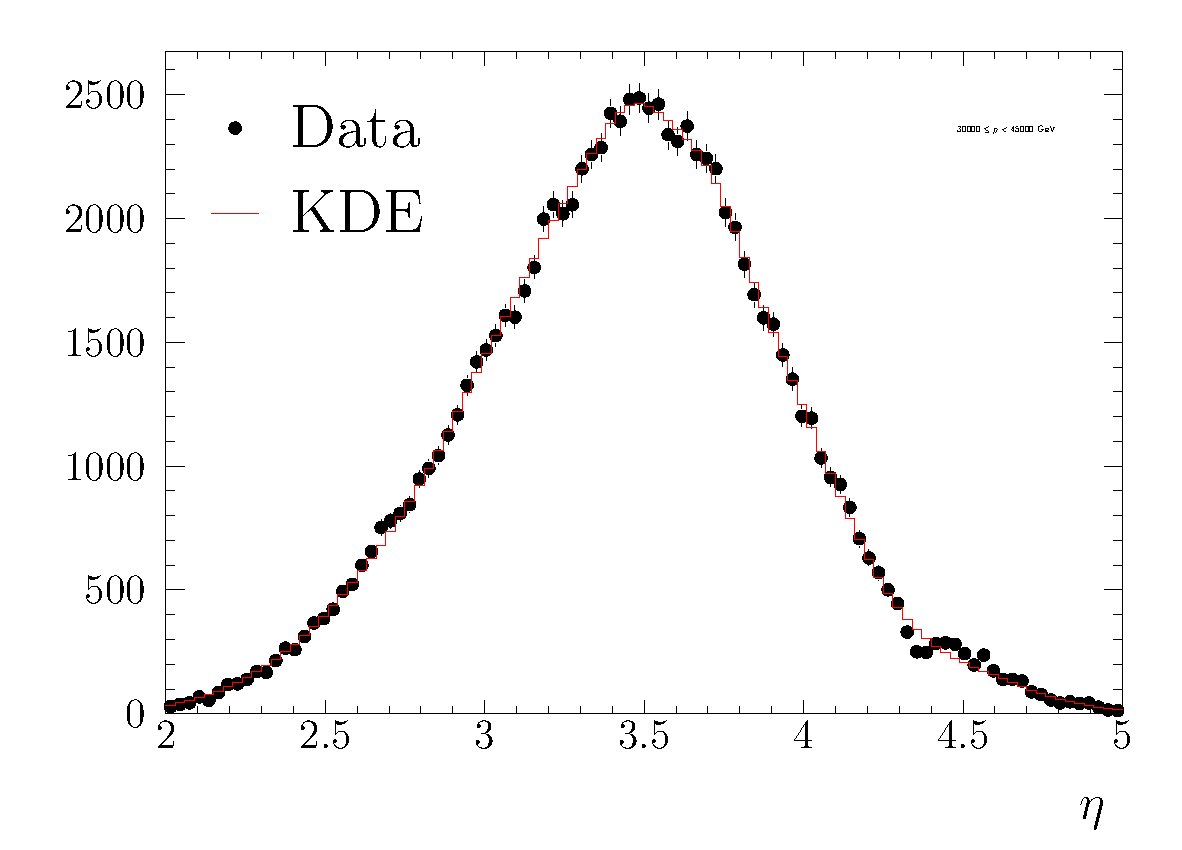
\includegraphics[width=\textwidth]{production/systematics/PIDK_binning_eta_bin3}
    \caption{\ptotrange{30}{45}}
    \label{fig:prod:syst:pid:kde_eta:bin3}
  \end{subfigure}
  \begin{subfigure}{0.5\textwidth}
    \centering
    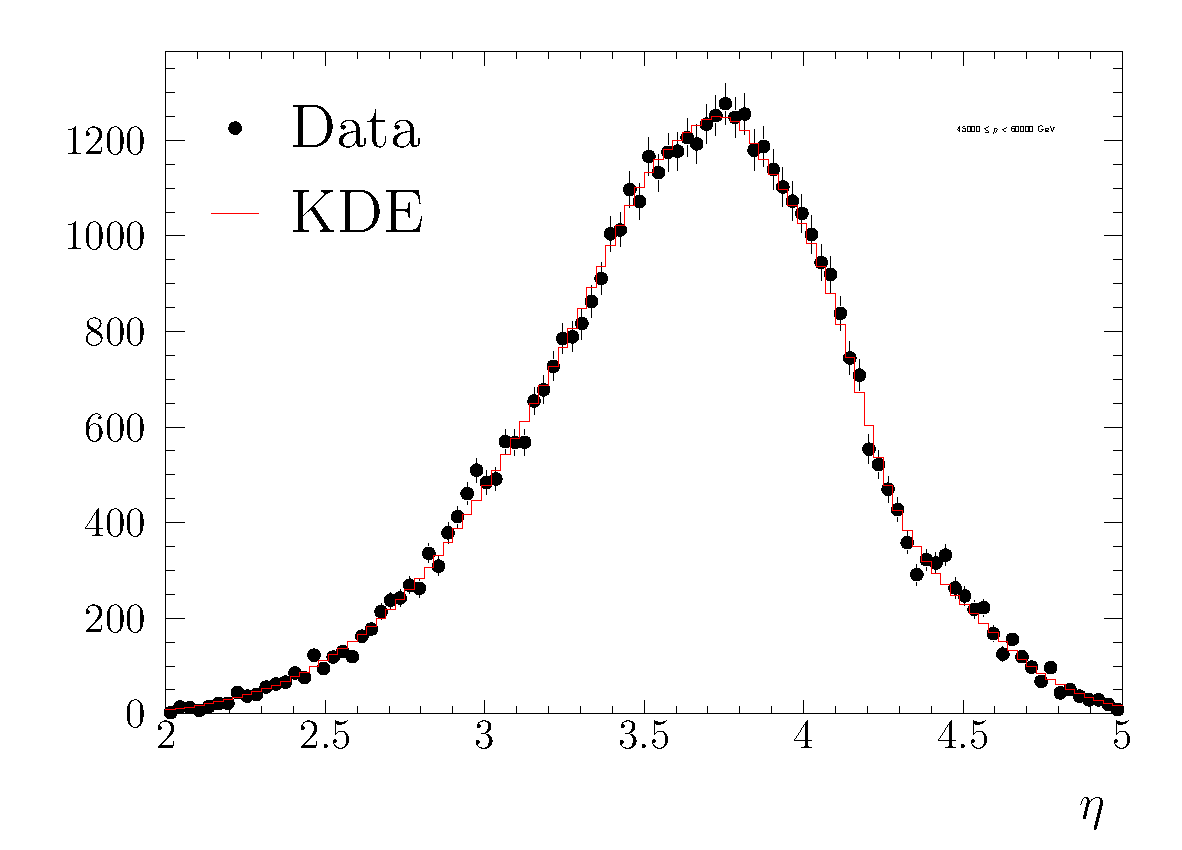
\includegraphics[width=\textwidth]{production/systematics/PIDK_binning_eta_bin4}
    \caption{\ptotrange{45}{60}}
    \label{fig:prod:syst:pid:kde_eta:bin4}
  \end{subfigure}
  \begin{subfigure}{0.5\textwidth}
    \centering
    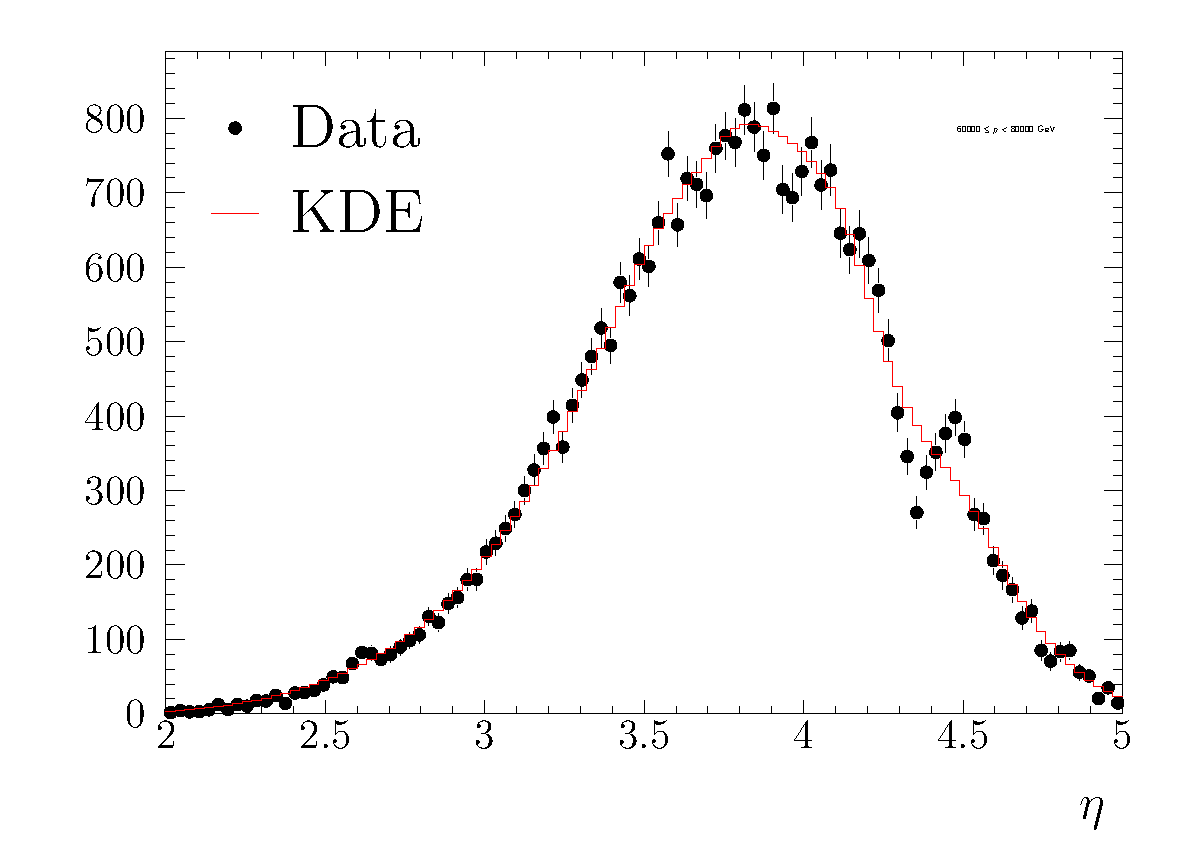
\includegraphics[width=\textwidth]{production/systematics/PIDK_binning_eta_bin5}
    \caption{\ptotrange{60}{80}}
    \label{fig:prod:syst:pid:kde_eta:bin5}
  \end{subfigure}
  \caption{%
    Pseudorapidity distribution in the kaon \ac{PID} signal calibration sample, 
    integrated across all values of kaon momentum 
    (\subref*{fig:prod:syst:pid:kde_eta:integrated}) and within a series of 
    smaller \ptot\ bins 
    (\subref*{fig:prod:syst:pid:kde_eta:bin1}--\subref*{fig:prod:syst:pid:kde_eta:bin5}).
  }
  \label{fig:prod:syst:pid:kde_eta}
\end{figure}

\begin{figure}
  \begin{subfigure}{0.5\textwidth}
    \centering
    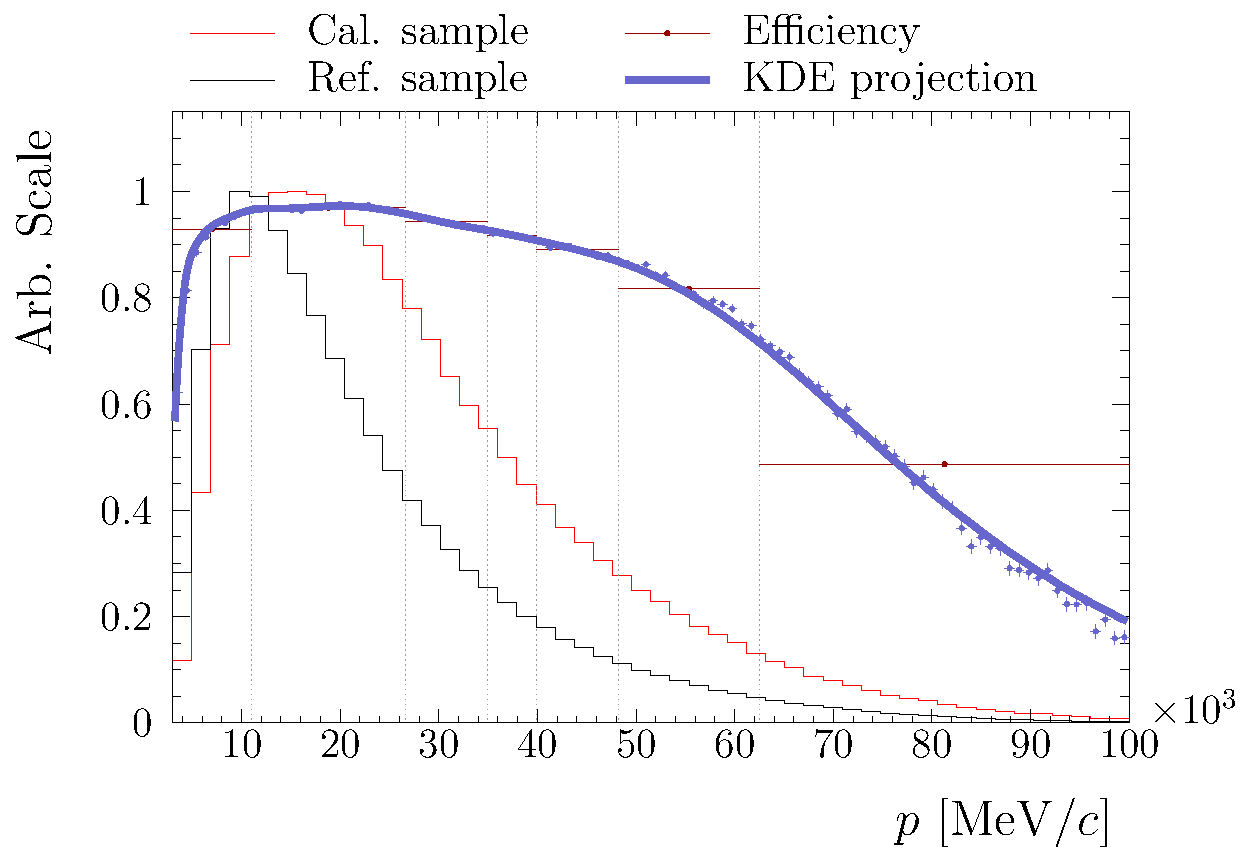
\includegraphics[width=\textwidth]{production/systematics/PIDK_binning_p}
    \caption{Kaon \ptot}
    \label{fig:prod:syst:pid:kde_1d_binning:kaon_p}
  \end{subfigure}
  \begin{subfigure}{0.5\textwidth}
    \centering
    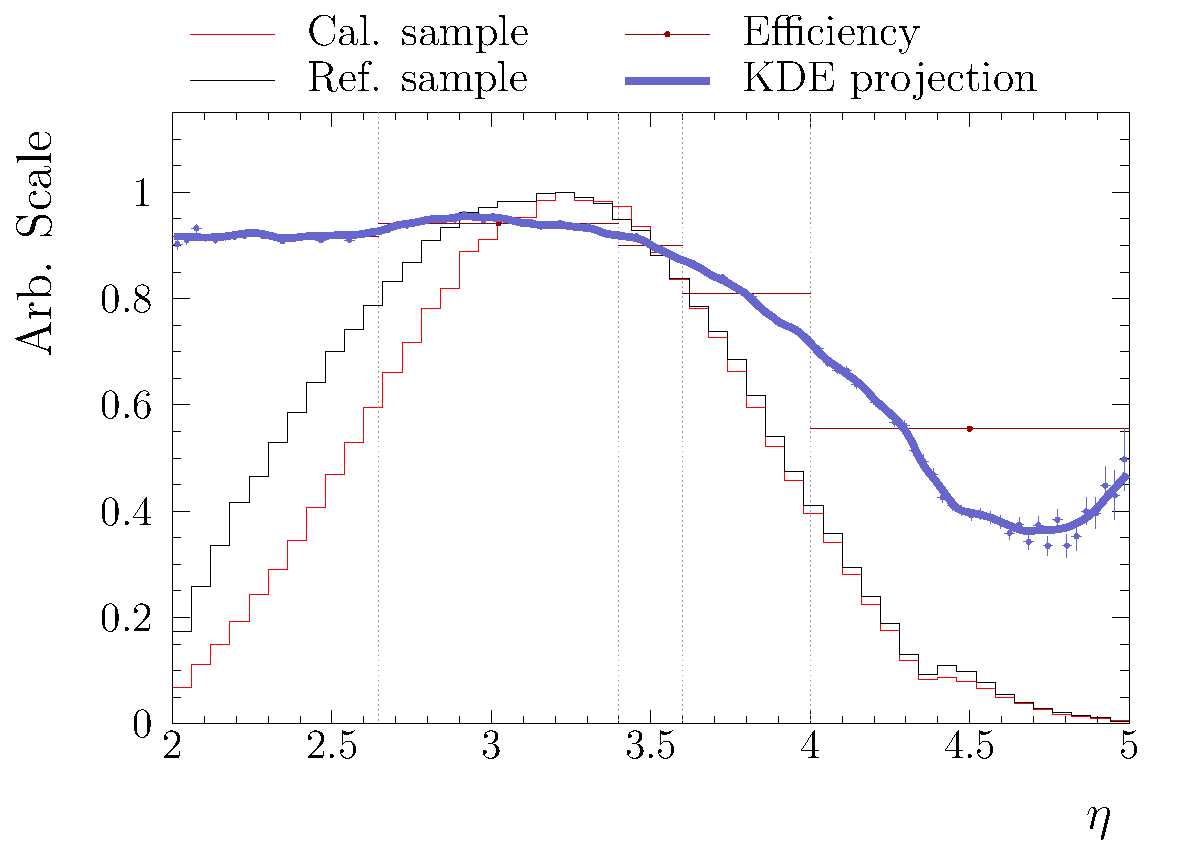
\includegraphics[width=\textwidth]{production/systematics/PIDK_binning_eta}
    \caption{Kaon \Eta}
    \label{fig:prod:syst:pid:kde_1d_binning:kaon_eta}
  \end{subfigure}
  \begin{subfigure}{0.5\textwidth}
    \centering
    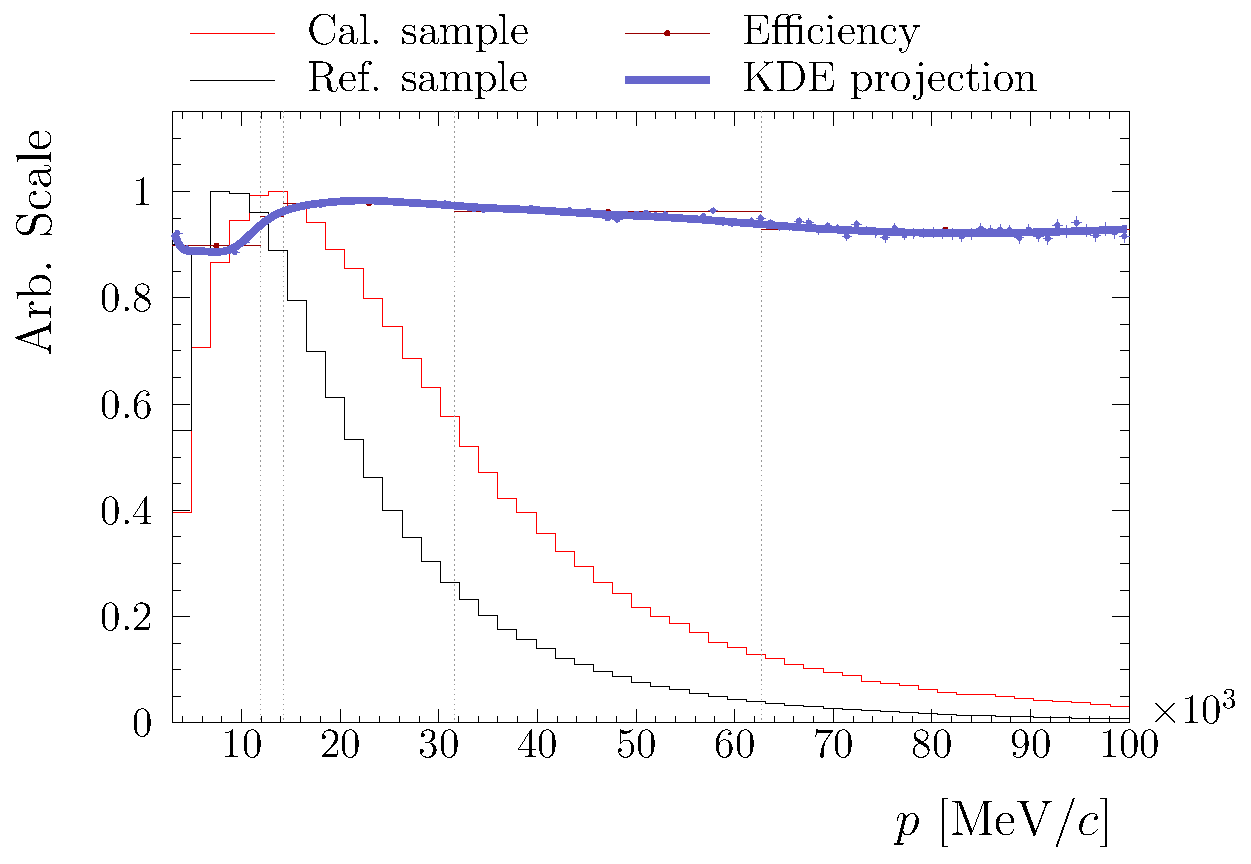
\includegraphics[width=\textwidth]{production/systematics/PIDpi_binning_p}
    \caption{Pion \ptot}
    \label{fig:prod:syst:pid:kde_1d_binning:pion_p}
  \end{subfigure}
  \begin{subfigure}{0.5\textwidth}
    \centering
    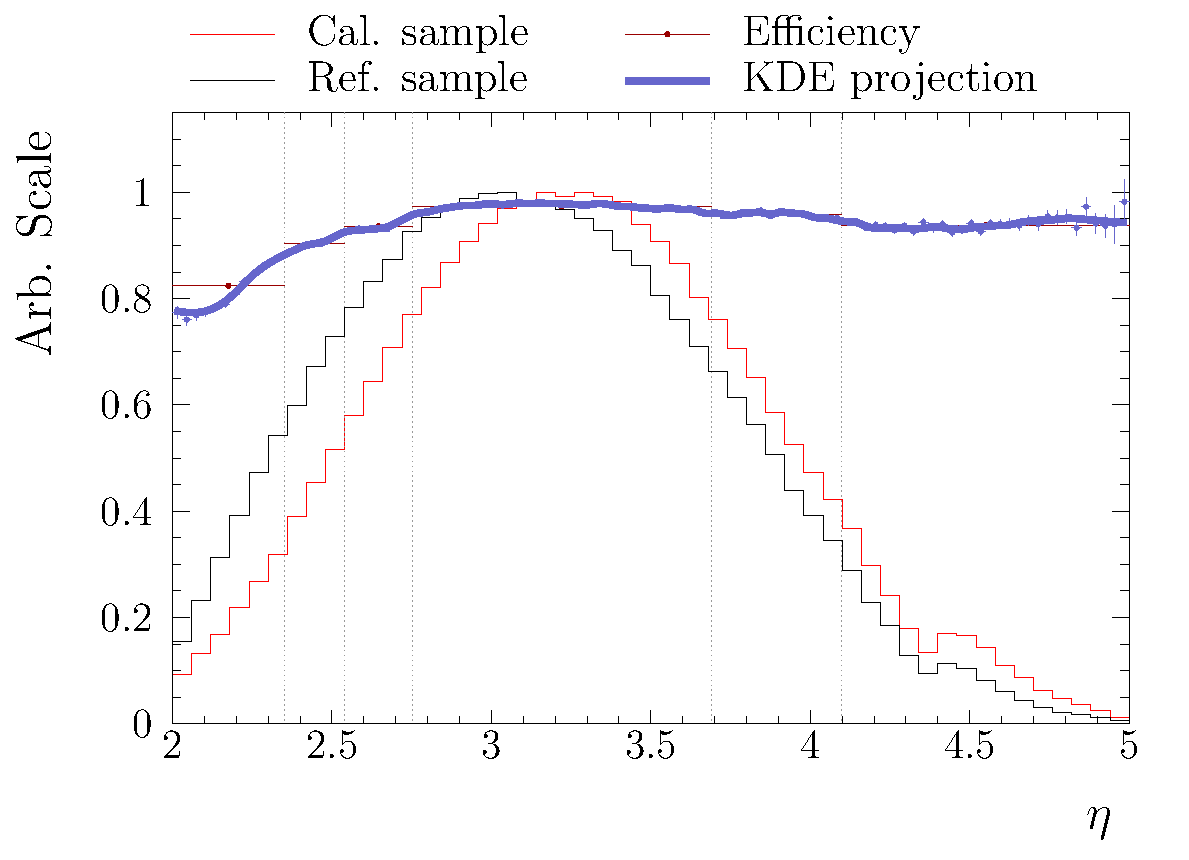
\includegraphics[width=\textwidth]{production/systematics/PIDpi_binning_eta}
    \caption{Pion \Eta}
    \label{fig:prod:syst:pid:kde_1d_binning:pion_eta}
  \end{subfigure}

  \caption{%
    As in \cref{fig:prod:pid:binning:kaon,fig:prod:pid:binning:pion}, but with 
    an estimate of the efficiency from \aclp{KDE} overlaid (blue curve).
  }
  \label{fig:prod:syst:pid:kde_1d_binning}
\end{figure}

\begin{figure}
  \begin{subfigure}{0.32\textwidth}
    \centering
    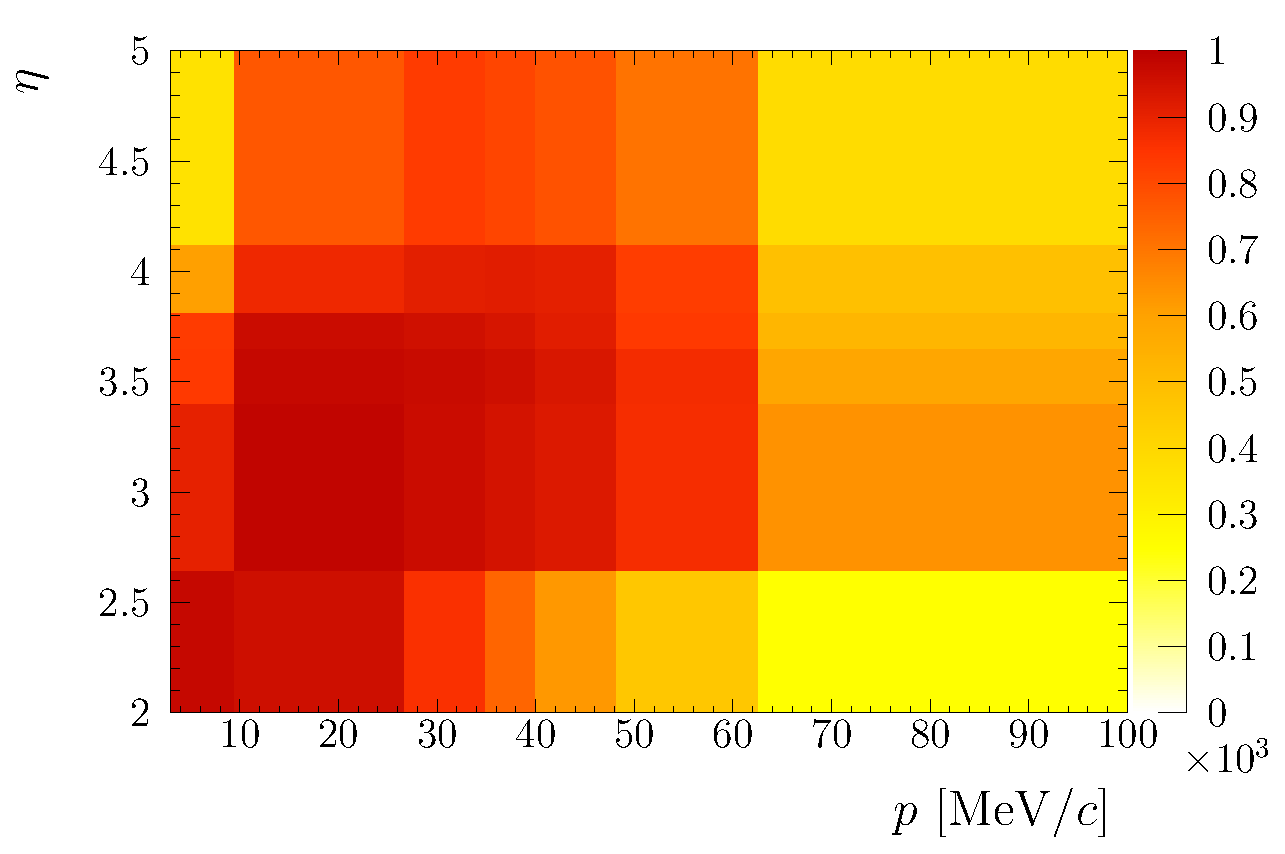
\includegraphics[width=\textwidth]{production/systematics/PIDK_binning_nominal}
    \caption{Nominal}
    \label{fig:prod:syst:pid:kde_2d_binning:kaon:nominal}
  \end{subfigure}
  \begin{subfigure}{0.32\textwidth}
    \centering
    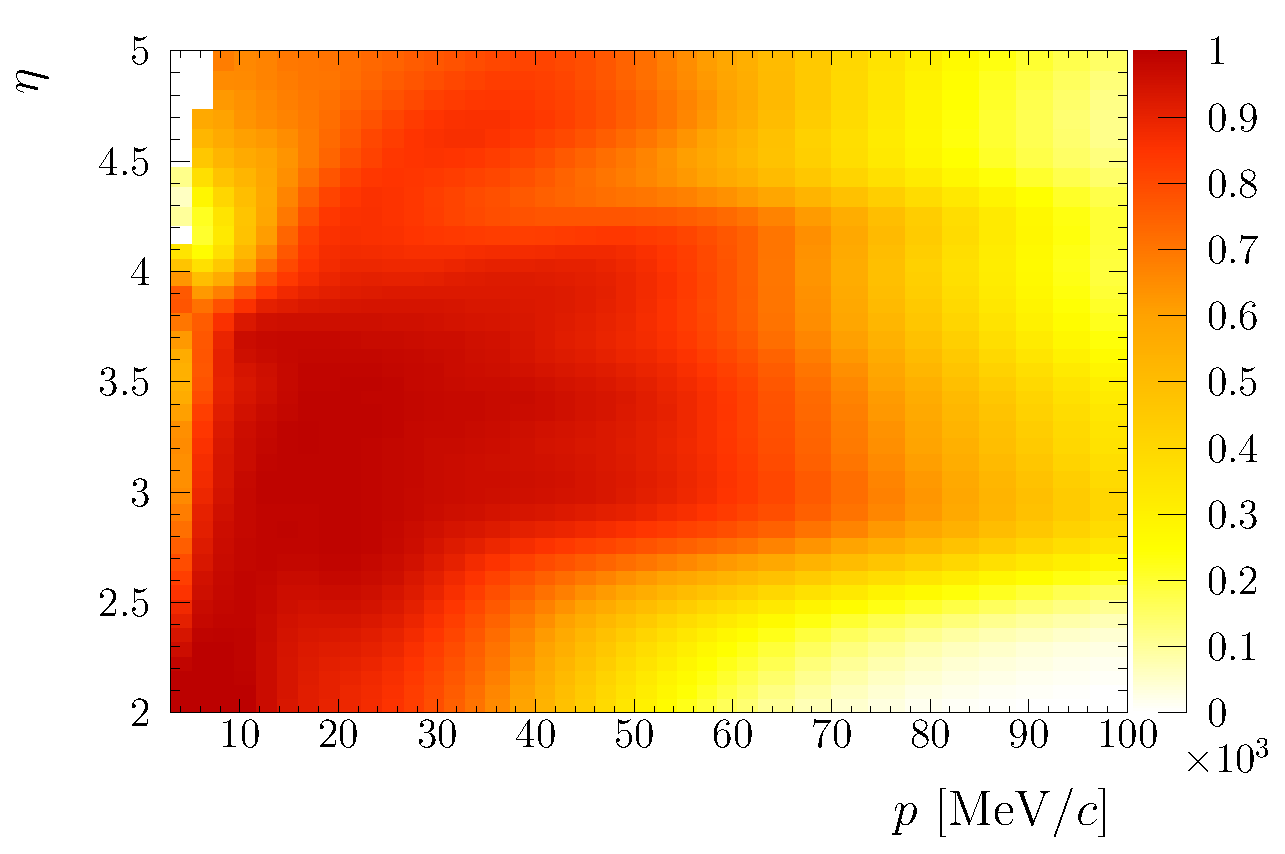
\includegraphics[width=\textwidth]{production/systematics/PIDK_binning_KDE_coarse}
    \caption{1221 bins}
    \label{fig:prod:syst:pid:kde_2d_binning:kaon:coarse}
  \end{subfigure}
  \begin{subfigure}{0.32\textwidth}
    \centering
    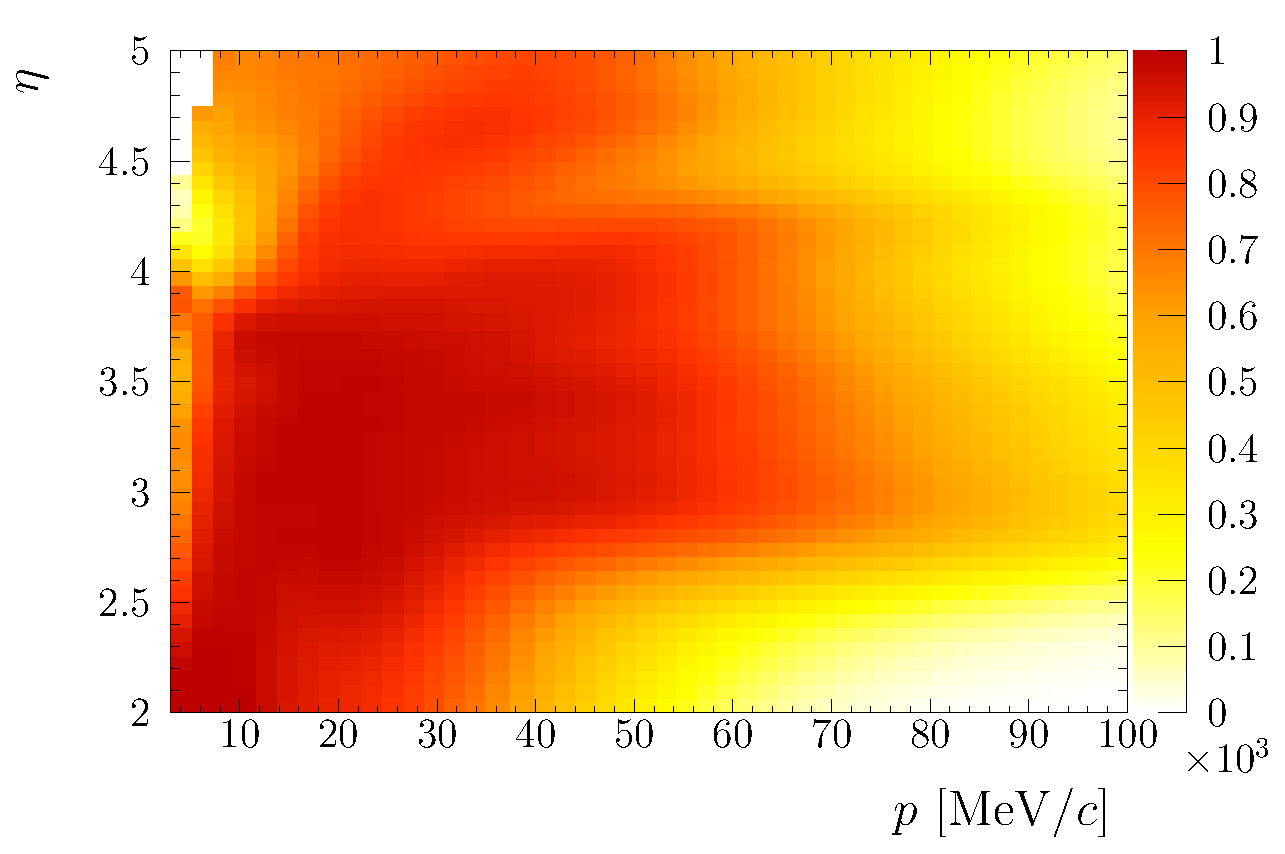
\includegraphics[width=\textwidth]{production/systematics/PIDK_binning_KDE_fine}
    \caption{2256 bins}
    \label{fig:prod:syst:pid:kde_2d_binning:kaon:fine}
  \end{subfigure}

  \caption{%
    Efficiency distributions $\eff_{i}(\ptot,\Eta)$ for kaon tracks in the 
    nominal binning scheme using the real calibration data 
    (\subref*{fig:prod:syst:pid:kde_2d_binning:kaon:nominal}) and higher 
    granularities using data generated from \aclp{KDE} 
    (\subref*{fig:prod:syst:pid:kde_2d_binning:kaon:coarse} and 
    \subref*{fig:prod:syst:pid:kde_2d_binning:kaon:fine}).
  }
  \label{fig:prod:syst:pid:kde_2d_binning:kaon}
\end{figure}

\begin{figure}
  \begin{subfigure}{0.32\textwidth}
    \centering
    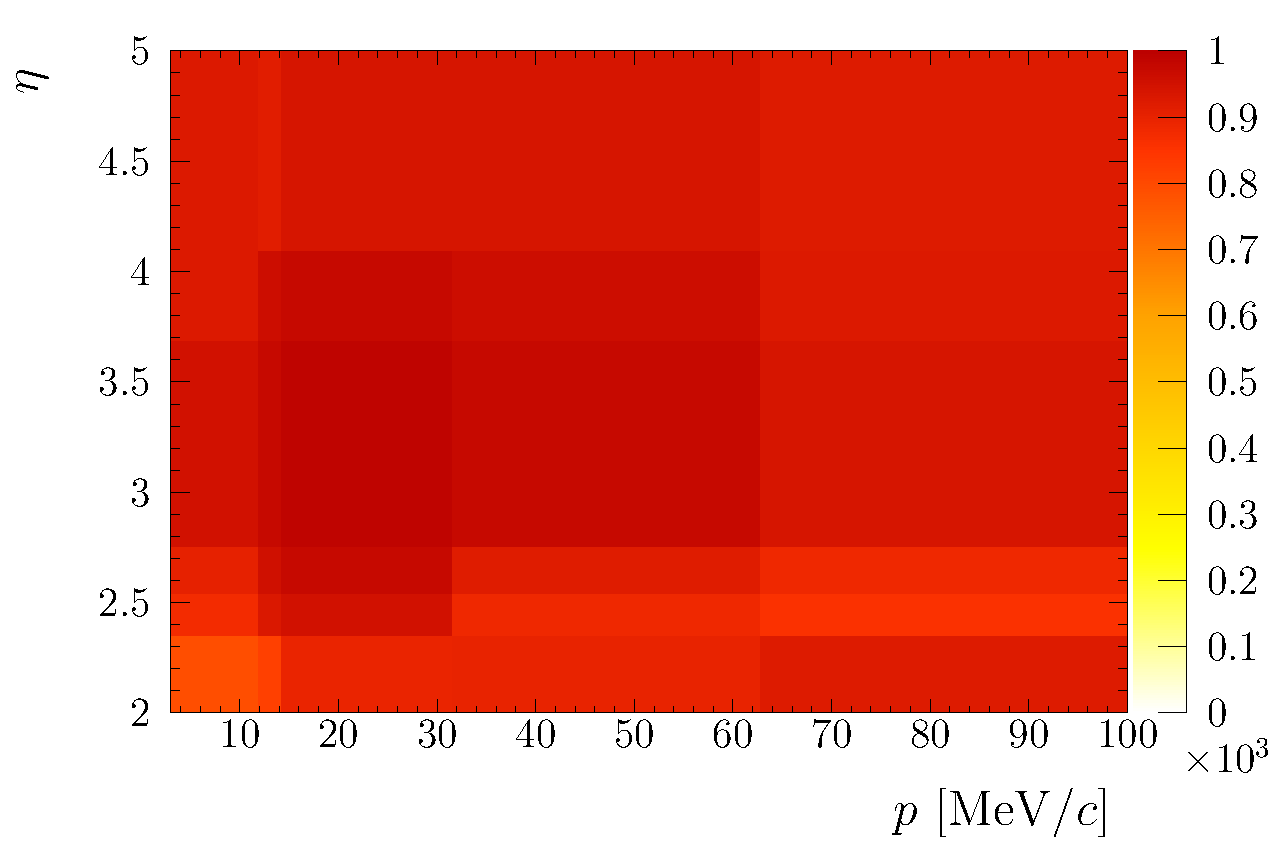
\includegraphics[width=\textwidth]{production/systematics/PIDpi_binning_nominal}
    \caption{Nominal}
    \label{fig:prod:syst:pid:kde_2d_binning:pion:nominal}
  \end{subfigure}
  \begin{subfigure}{0.32\textwidth}
    \centering
    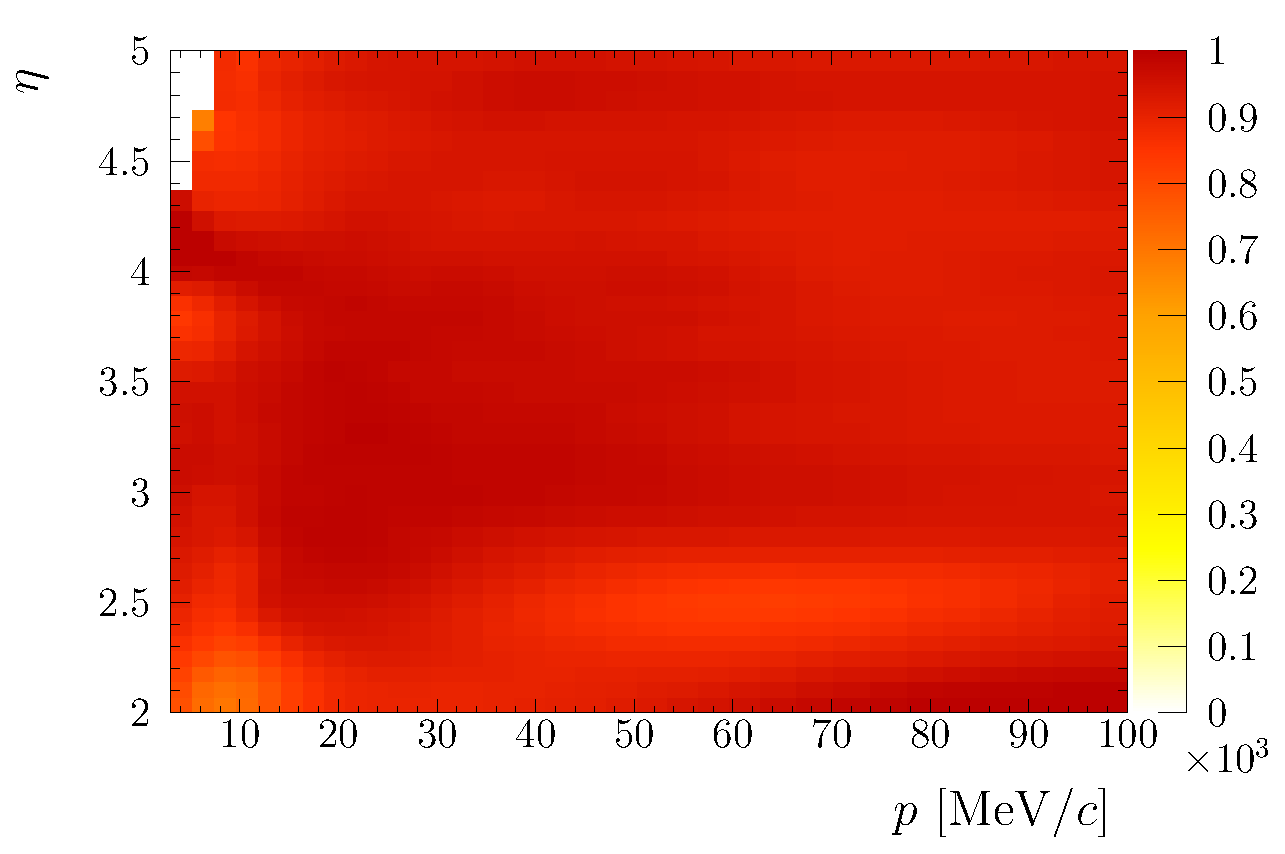
\includegraphics[width=\textwidth]{production/systematics/PIDpi_binning_KDE_coarse}
    \caption{960 bins}
    \label{fig:prod:syst:pid:kde_2d_binning:pion:coarse}
  \end{subfigure}
  \begin{subfigure}{0.32\textwidth}
    \centering
    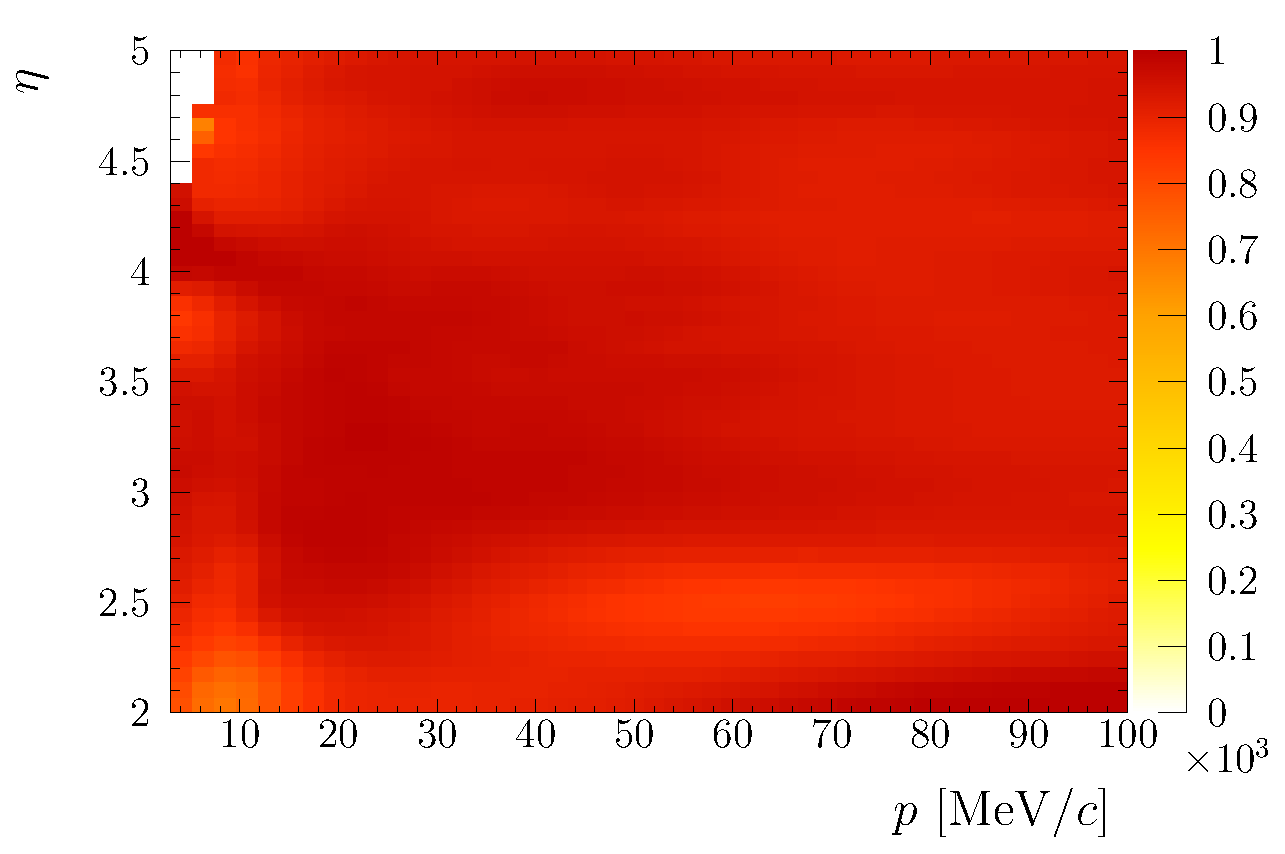
\includegraphics[width=\textwidth]{production/systematics/PIDpi_binning_KDE_fine}
    \caption{2162 bins}
    \label{fig:prod:syst:pid:kde_2d_binning:pion:fine}
  \end{subfigure}

  \caption{%
    Efficiency distributions $\eff_{i}(\ptot,\Eta)$ for pion tracks in the 
    nominal binning scheme using the real calibration data 
    (\subref*{fig:prod:syst:pid:kde_2d_binning:pion:nominal}) and higher 
    granularities using data generated from \aclp{KDE} 
    (\subref*{fig:prod:syst:pid:kde_2d_binning:pion:coarse} and 
    \subref*{fig:prod:syst:pid:kde_2d_binning:pion:fine}).
  }
  \label{fig:prod:syst:pid:kde_2d_binning:pion}
\end{figure}

\begin{figure}
  \begin{subfigure}{0.5\textwidth}
    \centering
    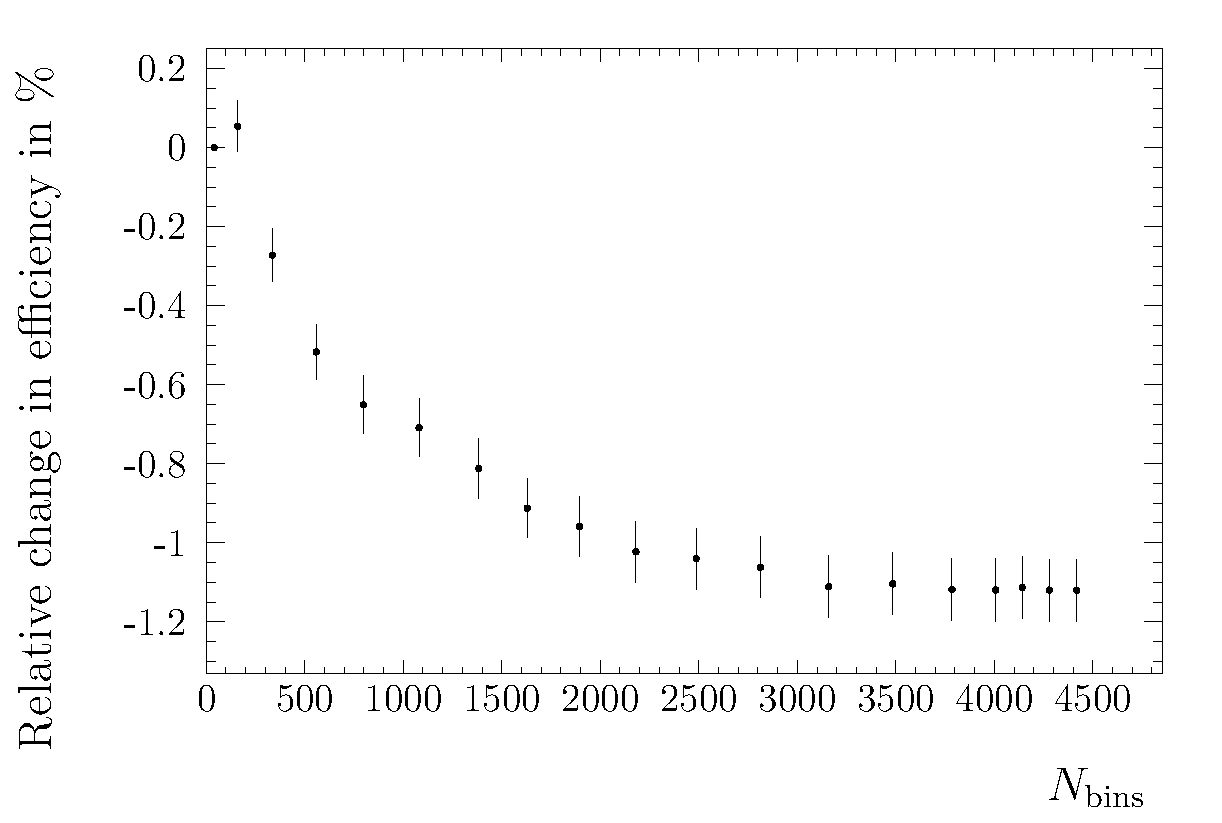
\includegraphics[width=\textwidth]{production/systematics/PIDK_binning_convergence}
    \caption{Kaon tracks}
    \label{fig:prod:syst:pid:convergence:kaon}
  \end{subfigure}
  \begin{subfigure}{0.5\textwidth}
    \centering
    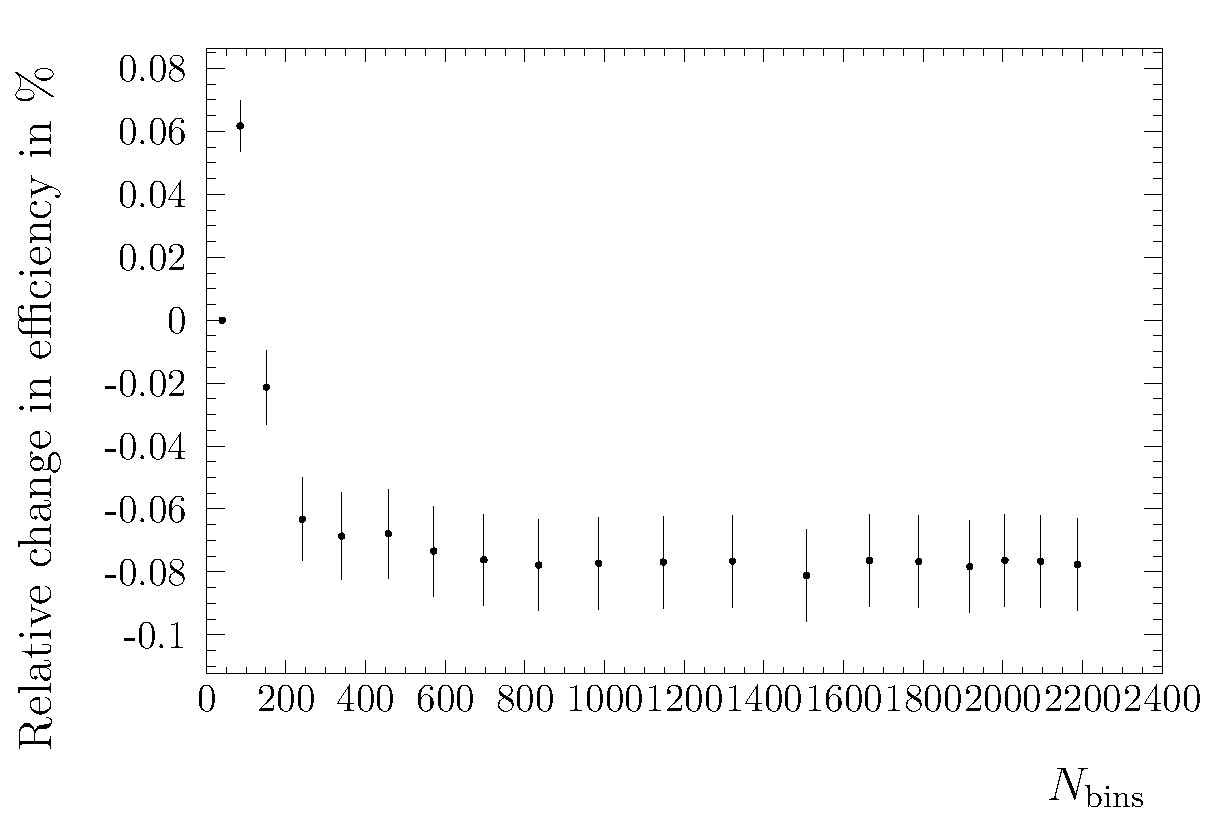
\includegraphics[width=\textwidth]{production/systematics/PIDpi_binning_convergence}
    \caption{Pion tracks}
    \label{fig:prod:syst:pid:convergence:pion}
  \end{subfigure}
  \caption{%
    Relative change in kaon (\subref*{fig:prod:syst:pid:convergence:kaon}) and 
    pion (\subref*{fig:prod:syst:pid:convergence:pion}) \ac{PID} efficiency 
    \effpid, as evaluated using \aclp{KDE}, when evaluated with a progressively 
    finer histogram binning.
  }
  \label{fig:prod:syst:pid:convergence}
\end{figure}


\section{Luminosity}
\label{chap:prod:syst:lumi}

The \acl{BGI} analysis described in \cref{chap:prod:data:lumi} comes with its 
own set of systematic uncertainties.
The dominant components arise from the limited resolution on the measurement of 
the beam-beam and beam-gas vertices, from the choice of fit model used to 
parameterise the transverse beam profiles, and the observed variation in 
measurements of the visible \pp\ cross-section over 
time~\cite{LHCb-PAPER-2014-047}.
The uncertainty on the luminosity measurement of \SI{3.8}{\%} is propagated to 
the cross-section measurements, and is fully correlated between all charm 
mesons and all \pTy\ bins.

\section{Tracking efficiency correction}
\label{chap:prod:syst:tracking}

The tracking efficiency corrections are computed as part of a dedicated 
analysis~\cite{Aaij:2014pwa}, summarised in \cref{chap:prod:effs:tracking}, and 
come with their own set of statistical and systematic uncertainties.

The statistical uncertainties on the correction factors, computed in bins of 
track \ptot\ and \Eta, and shown in \cref{fig:prod:effs:tracking_table}.
They are propagated to the cross-section measurements with pseudo-experiments 
in an identical manner to that used to propagate the statistical uncertainty on 
the \ac{PID} efficiency, as presented in \cref{chap:prod:syst:pid:stat}.
The use of pseudo-experiments encodes the intra- and inter-decay correlations 
of this uncertainty, and the resulting distribution of uncertainties is used as 
the \ac{PDF} of the corresponding parameter on the cross-sections.

The systematic uncertainty on the tracking efficiency correction factors is 
comprised of two components: that due to the difference between muon 
interactions with the detector (used to probe the efficiency) and those of 
hadrons (used in the cross-section measurements); and that due to the weighting 
procedure used to equalise the event multiplicity between the real data and the 
\ac{MC}.
For the former source, a systematic uncertainty of \SI{1.1}{\percent} is 
assigned per pion track and of \SI{1.4}{\percent} per kaon track, both of which 
are dominated by an assumed \SI{10}{\percent} uncertainty on the material 
budget in the simulation.
The latter source contributes \SI{0.4}{\percent}.
The corresponding nuisance parameters for both source are modelled as normal 
distributions.

Unlike the systematic uncertainties on the \ac{PID} efficiencies, the 
systematic uncertainties on the correction factors are highly correlated both 
between \pTy\ bins and between charm mesons.
This is due to the hadronic interaction and weighting uncertainties being 
dominant and global.
The systematic uncertainty on the tracking efficiency correction factor 
relative to the measured cross-section value is given in 
\cref{tab:prod:syst:tracking:D0ToKpi,tab:prod:syst:tracking:DpToKpipi} for 
\DzToKpi\ and \DpToKpipi.

\section{Branching fractions}
\label{chap:prod:syst:bf}

The branching fractions, provided by the Particle Data Group~\cite{PDG2014} and 
the \cleo\ collaboration~\cite{Alexander:2008aa} and listed in 
\cref{tab:prod:introduction:branching_ratios}, carry an uncertainty.
These are propagated as a systematic uncertainty on the cross-sections as 
normal distributions of mean of zero and width equal to the uncertainty.

\section{Fit model}
\label{chap:prod:syst:fitting}

The choice of \acp{PDF} used to model the data in the fitting procedure 
described in \cref{chap:prod:fitting} is somewhat arbitrary, in that they are 
not the only functional forms that will fit the data well.
The magnitude of the difference between the cross-sections computed with other 
fit models and the nominal model is assigned as a systematic uncertainty on the 
result.
This corresponds to an uncertainty on what the true generating \ac{PDF} is for 
the observed data.

With respect to the nominal signal model used in the \lnipchisq\ fit, from 
\cref{eqn:prod:fitting:ipchisq:signal_model}, alternative signal models used in 
the \lnipchisq\ fits are: \cref{eqn:prod:fitting:ipchisq:signal_model} where 
the Gaussian core is replaced by a `double Gaussian' core, which is the sum of 
two Gaussian distributions sharing a common mean but having independent widths; 
and a `smeared' $\ln{\chisq}$ distribution, obtained by modifying the usual 
\chisq\ functional form to have a parameterised asymmetry in the widths either 
side of the mean~\cite{LHCb-CONF-2016-010}.
Alternative models for the secondary charm component are the \ac{PDF} used for 
the prompt signal, and the asymmetric \chisq\ function used as an alternative 
prompt signal model.
No alternative models for the background component are tested.

The resulting relative systematic uncertainties are given in 
\cref{tab:syst:fitting:D0ToKpi,tab:syst:fitting:DpToKpipi} for \DzToKpi\ and 
\DpToKpipi.

\section{Signal window}
\label{chap:prod:syst:signal_window}

The signal window that is applied to the data entering the \lnipchisq\ fit, as 
described in \cref{chap:prod:fitting}, and this has an efficiency, as 
described in \cref{chap:prod:effs:signal_window}.
The computation of this efficiency assumes the signal model is known, but the 
parameters of the model are fitted to the data, and so have an uncertainty, 
which results in a systematic uncertainty on the signal window efficiency.

This computation of the uncertainty on the signal window efficiency is given in
\cref{chap:prod:effs:signal_window}.
This is is propagated the cross-sections as the systematic uncertainty, 
modelled as a normal distribution, and is given in 
\cref{tab:syst:signal_window:D0ToKpi,tab:syst:signal_window:DpToKpipi} relative 
to the cross-section values for \DzToKpi\ and \DpToKpipi.

\section{Correlations and summary}
\label{chap:prod:syst:correlations}

The different sources of systematic uncertainty that have been discussed in 
this \namecref{chap:prod:syst} can be grouped into three categories:
global uncertainties, which are correlated between all bins and all modes; 
uncertainties which are are only correlated
between the \pTy\ bins of a decay mode; and uncertainties which are 
uncorrelated between bins and modes.

Global uncertainties are from the luminosity, from the tracking efficiency 
correction factors, and the \DzToKpi\ branching fraction in between the 
\DzToKpi\ and \DstToDzpi\ with \DzToKpi\ measurements.
Correlated between bins within a decay mode are the uncertainties from the 
branching fractions, from the arbitrary choice of fit model, and from the 
\ac{PID} calibration sample size and binning scheme.
The uncertainty due to the finite \ac{MC} sample size is uncorrelated between 
bins and between modes.

A summary of the uncertainties entering the cross-section measurements, and 
their correlations, is given in \cref{tab:prod:syst:summary}.

\begin{table}
  \caption{%
    Systematic uncertainties expressed as fractions of the cross-section 
    measurements, in percent.
    Uncertainties that are computed bin-by-bin are expressed as ranges giving 
    the minimum to maximum values.
    Ranges for the correlations between \pTy\ bins and between modes are also 
    given, expressed in percent.
  }
  \label{tab:prod:syst:summary}
  \centering
  \begin{tabular}{lcccccc}
                         & \multicolumn{4}{c}{Uncertainties (\si{\percent})} & \multicolumn{2}{c}{Correlations (\si{\percent})} \\
                         & \PDzero                                           & \PDplus                                           & \PDsplus   & \PDstarp   & Bins    & Modes   \\
  \midrule
  Simulation sample size & 2--24                                             & 4--55                                             & 3--55      & 2--21      & -       & -       \\
  Simulation modelling   & 2                                                 & 1                                                 & 1          & 1          & -       & -       \\
  Truth sample size      & 0.02                                              & 0.18                                              & 0.11       & 0.08       & -       & -       \\
  \midrule
  Tracking               & 3--5                                              & 5--17                                             & 4--18      & 5--20      & 90--100 & 90--100 \\
  \ac{PID} sample size   & 0--2                                              & 0--1                                              & 0--2       & 0--1       & 0--100  & 0--100  \\
  \ac{PID} binning       & 0--44                                             & 0--10                                             & 0--20      & 0-15       & 100     & 100     \\
  \midrule
  PDF shapes             & 1--6                                              & 1--5                                              & 1--2       & 1--2       & -       & -       \\
  Signal window          & 0.04--0.4                                         & 0.04--1.7                                         & 0.06--1.4  & 0.16--2.84 & -       & -       \\
  \midrule
  Branching fractions    & 1.2                                               & 2.1                                               & 5.8        & 1.5        & 100     & 0--95   \\
  Luminosity             & \multicolumn{4}{c}{3.9}                           & 100                                               & 100       \\
\end{tabular}

\end{table}

\begin{table}
  \caption{%
    Relative uncertainty on the \PDzero cross-section, in \PDzero \pTy\ bins, 
    due to the finite size of the Monte Carlo sample used to assess the 
    selection efficiency.
  }
  \label{tab:prod:syst:mc:stat:D0ToKpi}
  \centering
  \renewcommand{\arraystretch}{1.0}
\begin{tabular}{lccccc}
\toprule&\multicolumn{5}{c}{$\text{$y$}$}\\
$\text{$p_{\text{T}}$ [\text{MeV}/c]}$ & $[2,2.5[$ & $[2.5,3[$ & $[3,3.5[$ & $[3.5,4[$ & $[4,4.5[$ \\
\midrule$[0,1000[$ & $3.91$ & $1.81$ & $1.62$ & $2.07$ & $4.66$ \\
$[1000,1500[$ & $3.77$ & $1.83$ & $1.63$ & $2.02$ & $3.87$ \\
$[1500,2000[$ & $3.39$ & $1.69$ & $1.54$ & $1.96$ & $3.57$ \\
$[2000,2500[$ & $3.02$ & $1.61$ & $1.52$ & $1.85$ & $3.31$ \\
$[2500,3000[$ & $2.83$ & $1.56$ & $1.47$ & $1.84$ & $3.40$ \\
$[3000,3500[$ & $2.82$ & $1.58$ & $1.52$ & $1.89$ & $3.52$ \\
$[3500,4000[$ & $2.82$ & $1.62$ & $1.64$ & $2.01$ & $4.06$ \\
$[4000,5000[$ & $2.14$ & $1.31$ & $1.32$ & $1.62$ & $4.34$ \\
$[5000,6000[$ & $2.53$ & $1.68$ & $1.62$ & $2.20$ & $8.15$ \\
$[6000,7000[$ & $2.96$ & $2.06$ & $2.05$ & $3.23$ & $24.57$ \\
$[7000,8000[$ & $3.56$ & $2.61$ & $2.70$ & $5.06$ & - \\
$[8000,9000[$ & $4.55$ & $3.17$ & $3.56$ & $10.00$ & - \\
$[9000,10000[$ & $1.39$ & $1.03$ & $1.24$ & $4.52$ & - \\
$[10000,11000[$ & $1.44$ & $1.08$ & $1.45$ & $7.33$ & - \\
$[11000,12000[$ & $1.74$ & $1.37$ & $2.11$ & - & - \\
$[12000,13000[$ & $2.00$ & $1.75$ & $3.18$ & - & - \\
$[13000,14000[$ & $2.54$ & $2.28$ & $4.38$ & - & - \\
$[14000,15000[$ & $2.85$ & $2.96$ & $6.51$ & - & - \\
\bottomrule\end{tabular}

\end{table}

\begin{table}
  \caption{%
    Relative uncertainty on the \PDplus cross-section, in \PDplus \pTy\ bins, 
    due to the finite size of the Monte Carlo sample used to assess the 
    selection efficiency.
  }
  \label{tab:prod:syst:mc:stat:DpToKpipi}
  \centering
  \renewcommand{\arraystretch}{1.0}
\begin{tabular}{lccccc}
\toprule&\multicolumn{5}{c}{$\text{$y$}$}\\
$\text{$p_{\text{T}}$ [\text{MeV}/c]}$ & $[2,2.5]$ & $[2.5,3]$ & $[3,3.5]$ & $[3.5,4]$ & $[4,4.5]$ \\
\midrule
$[0,1000]$ & $55.08$ & $15.49$ & $9.88$ & $9.94$ & $21.48$ \\
$[1000,1500]$ & $18.04$ & $4.93$ & $3.43$ & $3.84$ & $7.29$ \\
$[1500,2000]$ & $8.85$ & $2.53$ & $1.98$ & $2.25$ & $4.53$ \\
$[2000,2500]$ & $5.00$ & $1.83$ & $1.51$ & $1.75$ & $3.29$ \\
$[2500,3000]$ & $4.05$ & $1.59$ & $1.36$ & $1.58$ & $2.91$ \\
$[3000,3500]$ & $3.64$ & $1.60$ & $1.40$ & $1.62$ & $2.95$ \\
$[3500,4000]$ & $3.34$ & $1.64$ & $1.46$ & $1.72$ & $3.16$ \\
$[4000,5000]$ & $2.47$ & $1.29$ & $1.19$ & $1.41$ & $2.73$ \\
$[5000,6000]$ & $2.78$ & $1.56$ & $1.50$ & $1.78$ & $4.25$ \\
$[6000,7000]$ & $3.21$ & $1.89$ & $1.88$ & $2.48$ & $7.39$ \\
$[7000,8000]$ & $3.69$ & $2.36$ & $2.36$ & $3.31$ & $16.04$ \\
$[8000,9000]$ & $4.55$ & $2.91$ & $3.01$ & $4.87$ & $34.43$ \\
$[9000,10000]$ & $4.46$ & $2.89$ & $2.87$ & $5.40$ & - \\
$[10000,11000]$ & $1.29$ & $0.93$ & $1.03$ & $2.50$ & - \\
$[11000,12000]$ & $1.44$ & $1.17$ & $1.51$ & $3.71$ & - \\
$[12000,13000]$ & $1.79$ & $1.40$ & $1.92$ & $5.94$ & - \\
$[13000,14000]$ & $2.22$ & $2.00$ & $2.50$ & $11.93$ & - \\
$[14000,15000]$ & $2.87$ & $2.44$ & $3.53$ & - & - \\
\bottomrule\end{tabular}

\end{table}

\begin{table}
  \caption{%
    Relative uncertainties on the charm cross-sections $\xsec(\PHc)$ due to the 
    mis-modelling of the data in the Monte Carlo sample.
  }
  \label{tab:prod:syst:mc:modelling}
  \centering
  \begin{tabular}{lr}
  \toprule
  Decay mode                & Relative error      \\
  \midrule
  \DzToKpi                  & \SI{1.1}{\percent}  \\
  \DpToKpipi                & \SI{1.2}{\percent}  \\
  \DspTophipi               & \SI{0.2}{\percent}  \\
  \DstToDzpi\ with \DzToKpi & \SI{0.91}{\percent} \\
  \bottomrule
\end{tabular}

\end{table}

\begin{table}
  \caption{%
    Relative uncertainties on the charm cross-sections $\xsec(\PHc)$ due to the 
    finite size of the Monte Carlo sample used to assess the truth matching 
    efficiency.
  }
  \label{tab:prod:syst:mc:truth_matching}
  \centering
  \begin{tabular}{lr}
  \toprule
  Decay mode                & Relative error      \\
  \midrule
  \DzToKpi                  & \SI{0.02}{\percent} \\
  \DpToKpipi                & \SI{0.18}{\percent} \\
  \DspTophipi               & \SI{0.11}{\percent} \\
  \DstToDzpi\ with \DzToKpi & \SI{0.08}{\percent} \\
  \bottomrule
\end{tabular}

\end{table}

\begin{table}
  \caption{%
    Relative uncertainty on the \PDzero cross-section, in \PDzero \pTy\ bins, 
    due to the finite size of the \ac{PID} calibration sample.
  }
  \label{tab:syst:pid:stat:D0ToKpi}
  \centering
  \renewcommand{\arraystretch}{1.0}
\begin{tabular}{lccccc}
\toprule&\multicolumn{5}{c}{$\text{$y$}$}\\
$\text{$p_{\text{T}}$ [\text{MeV}/c]}$ & $[2,2.5]$ & $[2.5,3]$ & $[3,3.5]$ & $[3.5,4]$ & $[4,4.5]$ \\
\midrule
$[0,1000]$ & $0.22$ & $0.19$ & $0.11$ & $0.16$ & $0.29$ \\
$[1000,1500]$ & $0.21$ & $0.15$ & $0.11$ & $0.13$ & $0.25$ \\
$[1500,2000]$ & $0.21$ & $0.12$ & $0.09$ & $0.11$ & $0.27$ \\
$[2000,2500]$ & $0.21$ & $0.10$ & $0.07$ & $0.10$ & $0.33$ \\
$[2500,3000]$ & $0.20$ & $0.08$ & $0.06$ & $0.11$ & $0.37$ \\
$[3000,3500]$ & $0.18$ & $0.07$ & $0.06$ & $0.12$ & $0.42$ \\
$[3500,4000]$ & $0.17$ & $0.07$ & $0.05$ & $0.14$ & $0.45$ \\
$[4000,5000]$ & $0.16$ & $0.06$ & $0.06$ & $0.19$ & $0.50$ \\
$[5000,6000]$ & $0.15$ & $0.06$ & $0.08$ & $0.24$ & $0.57$ \\
$[6000,7000]$ & $0.17$ & $0.08$ & $0.13$ & $0.29$ & $0.62$ \\
$[7000,8000]$ & $0.19$ & $0.12$ & $0.19$ & $0.36$ & - \\
$[8000,9000]$ & $0.23$ & $0.17$ & $0.24$ & $0.44$ & - \\
$[9000,10000]$ & $0.28$ & $0.31$ & $0.29$ & $0.51$ & - \\
$[10000,11000]$ & $0.41$ & $0.38$ & $0.35$ & $0.79$ & - \\
$[11000,12000]$ & $0.50$ & $0.65$ & $0.44$ & - & - \\
$[12000,13000]$ & $0.63$ & $1.01$ & $0.50$ & - & - \\
$[13000,14000]$ & $0.75$ & $1.57$ & $0.56$ & - & - \\
$[14000,15000]$ & $1.20$ & $2.01$ & $0.67$ & - & - \\
\bottomrule\end{tabular}

\end{table}

\begin{table}
  \caption{%
    Relative uncertainty on the \PDplus cross-section, in \PDplus \pTy\ bins, 
    due to the finite size of the \ac{PID} calibration sample.
  }
  \label{tab:syst:pid:stat:DpToKpipi}
  \centering
  \renewcommand{\arraystretch}{1.0}
\begin{tabular}{l|ccccc}
\toprule&\multicolumn{5}{c}{$\text{$y$}$}\\
$\text{$p_{\text{T}}$ [\text{MeV}/c]}$ & $[2,2.5[$ & $[2.5,3[$ & $[3,3.5[$ & $[3.5,4[$ & $[4,4.5[$ \\
\midrule$[0,1000[$ & $0.30$ & $0.30$ & $0.36$ & $0.52$ & $0.62$ \\
$[1000,1500[$ & $0.29$ & $0.29$ & $0.44$ & $0.44$ & $0.46$ \\
$[1500,2000[$ & $0.31$ & $0.27$ & $0.35$ & $0.34$ & $0.37$ \\
$[2000,2500[$ & $0.34$ & $0.23$ & $0.24$ & $0.24$ & $0.33$ \\
$[2500,3000[$ & $0.35$ & $0.20$ & $0.17$ & $0.19$ & $0.30$ \\
$[3000,3500[$ & $0.35$ & $0.18$ & $0.13$ & $0.16$ & $0.31$ \\
$[3500,4000[$ & $0.34$ & $0.16$ & $0.11$ & $0.15$ & $0.34$ \\
$[4000,5000[$ & $0.32$ & $0.13$ & $0.08$ & $0.14$ & $0.39$ \\
$[5000,6000[$ & $0.29$ & $0.11$ & $0.08$ & $0.16$ & $0.47$ \\
$[6000,7000[$ & $0.28$ & $0.10$ & $0.09$ & $0.20$ & $0.53$ \\
$[7000,8000[$ & $0.27$ & $0.09$ & $0.11$ & $0.24$ & $0.59$ \\
$[8000,9000[$ & $0.28$ & $0.11$ & $0.14$ & $0.29$ & $0.81$ \\
$[9000,10000[$ & $0.28$ & $0.13$ & $0.16$ & $0.33$ & - \\
$[10000,11000[$ & $0.31$ & $0.18$ & $0.20$ & $0.39$ & - \\
$[11000,12000[$ & $0.35$ & $0.31$ & $0.23$ & $0.44$ & - \\
$[12000,13000[$ & $0.38$ & $0.38$ & $0.28$ & $0.50$ & - \\
$[13000,14000[$ & $0.47$ & $0.30$ & $0.32$ & $0.91$ & - \\
$[14000,15000[$ & $0.63$ & $0.52$ & $0.36$ & - & - \\
\bottomrule\end{tabular}

\end{table}

\begin{table}
  \caption{%
    Relative uncertainty on the \PDzero cross-section, in \PDzero \pTy\ bins, 
    due to the choice of \ac{PID} calibration binning.
  }
  \label{tab:syst:pid:binning:D0ToKpi}
  \centering
  \renewcommand{\arraystretch}{1.0}
\begin{tabular}{l|ccccc}
\toprule&\multicolumn{5}{c}{$\text{$y$}$}\\
$\text{$p_{\text{T}}$ [\text{MeV}/c]}$ & $[2,2.5[$ & $[2.5,3[$ & $[3,3.5[$ & $[3.5,4[$ & $[4,4.5[$ \\
\midrule$[0,1000[$ & $1.15$ & $0.09$ & $0.23$ & $0.74$ & $2.13$ \\
$[1000,1500[$ & $1.43$ & $0.98$ & $0.33$ & $0.26$ & $1.86$ \\
$[1500,2000[$ & $0.80$ & $0.44$ & $0.11$ & $0.34$ & $0.00$ \\
$[2000,2500[$ & $0.52$ & $0.11$ & $0.14$ & $0.88$ & $0.05$ \\
$[2500,3000[$ & $0.56$ & $0.39$ & $0.31$ & $2.00$ & $2.28$ \\
$[3000,3500[$ & $0.88$ & $0.53$ & $0.51$ & $2.95$ & $3.90$ \\
$[3500,4000[$ & $1.26$ & $0.51$ & $0.73$ & $2.79$ & $7.21$ \\
$[4000,5000[$ & $1.58$ & $0.40$ & $1.28$ & $1.41$ & $10.83$ \\
$[5000,6000[$ & $1.89$ & $0.15$ & $2.10$ & $1.65$ & $17.34$ \\
$[6000,7000[$ & $1.93$ & $0.20$ & $1.83$ & $5.37$ & $44.91$ \\
$[7000,8000[$ & $2.26$ & $0.49$ & $0.67$ & $10.51$ & - \\
$[8000,9000[$ & $2.54$ & $0.38$ & $0.37$ & $12.97$ & - \\
$[9000,10000[$ & $3.22$ & $0.05$ & $0.68$ & $24.15$ & - \\
$[10000,11000[$ & $4.47$ & $0.34$ & $3.82$ & $30.49$ & - \\
$[11000,12000[$ & $4.96$ & $0.29$ & $3.91$ & - & - \\
$[12000,13000[$ & $7.81$ & $0.32$ & $4.69$ & - & - \\
$[13000,14000[$ & $7.47$ & $0.00$ & $11.38$ & - & - \\
$[14000,15000[$ & $6.43$ & $3.10$ & $13.40$ & - & - \\
\bottomrule\end{tabular}

\end{table}

\begin{table}
  \caption{%
    Relative uncertainty on the \PDplus cross-section, in \PDplus \pTy\ bins, 
    due to the choice of \ac{PID} calibration binning.
  }
  \label{tab:syst:pid:binning:DpToKpipi}
  \centering
  \renewcommand{\arraystretch}{1.0}
\begin{tabular}{l|ccccc}
\toprule&\multicolumn{5}{c}{$\text{$y$}$}\\
$\text{$p_{\text{T}}$ [\text{MeV}/c]}$ & $[2,2.5[$ & $[2.5,3[$ & $[3,3.5[$ & $[3.5,4[$ & $[4,4.5[$ \\
\midrule$[0,1000[$ & $0.00$ & $3.88$ & $1.29$ & $1.61$ & $6.62$ \\
$[1000,1500[$ & $9.07$ & $8.28$ & $2.51$ & $2.57$ & $4.27$ \\
$[1500,2000[$ & $6.64$ & $5.45$ & $2.23$ & $1.72$ & $2.78$ \\
$[2000,2500[$ & $3.94$ & $3.03$ & $1.32$ & $1.04$ & $1.69$ \\
$[2500,3000[$ & $2.82$ & $1.05$ & $0.57$ & $0.18$ & $2.04$ \\
$[3000,3500[$ & $2.01$ & $0.20$ & $0.13$ & $0.61$ & $1.99$ \\
$[3500,4000[$ & $1.71$ & $0.32$ & $0.04$ & $1.36$ & $2.15$ \\
$[4000,5000[$ & $1.50$ & $0.79$ & $0.44$ & $1.72$ & $1.57$ \\
$[5000,6000[$ & $1.34$ & $1.00$ & $0.98$ & $1.15$ & $2.61$ \\
$[6000,7000[$ & $1.19$ & $0.84$ & $1.32$ & $0.38$ & $0.00$ \\
$[7000,8000[$ & $1.29$ & $0.57$ & $1.08$ & $2.03$ & $8.74$ \\
$[8000,9000[$ & $1.57$ & $0.32$ & $0.75$ & $3.19$ & $0.00$ \\
$[9000,10000[$ & $1.74$ & $0.27$ & $0.35$ & $5.55$ & - \\
$[10000,11000[$ & $2.00$ & $0.00$ & $0.00$ & $7.63$ & - \\
$[11000,12000[$ & $2.58$ & $0.00$ & $0.00$ & $4.19$ & - \\
$[12000,13000[$ & $3.08$ & $0.40$ & $0.00$ & $11.46$ & - \\
$[13000,14000[$ & $3.51$ & $0.63$ & $0.00$ & $0.00$ & - \\
$[14000,15000[$ & $3.53$ & $1.31$ & $0.02$ & - & - \\
\bottomrule\end{tabular}

\end{table}

\begin{table}
  \caption{%
    Relative uncertainty on the \PDzero cross-section, in \PDzero \pTy\ bins, 
    due to the finite calibration sample size, hadronic interaction 
    uncertainty, and event multiplicity weighting in the tracking efficiency 
    correction factor analysis.
  }
  \label{tab:prod:syst:tracking:D0ToKpi}
  \centering
  \renewcommand{\arraystretch}{1.0}
\begin{tabular}{lr@{\hskip+0.2em}c@{\hskip+0.2em}r@{\hskip+0.2em}c@{\hskip+0.2em}rr@{\hskip+0.2em}c@{\hskip+0.2em}r@{\hskip+0.2em}c@{\hskip+0.2em}rr@{\hskip+0.2em}c@{\hskip+0.2em}r@{\hskip+0.2em}c@{\hskip+0.2em}rr@{\hskip+0.2em}c@{\hskip+0.2em}r@{\hskip+0.2em}c@{\hskip+0.2em}rr@{\hskip+0.2em}c@{\hskip+0.2em}r@{\hskip+0.2em}c@{\hskip+0.2em}r}
\toprule&\multicolumn{25}{c}{$\text{$y$}$}\\
$\text{$p_{\text{T}}$ [\text{MeV}/c]}$ & \multicolumn{5}{c}{$[2,2.5]$} & \multicolumn{5}{c}{$[2.5,3]$} & \multicolumn{5}{c}{$[3,3.5]$} & \multicolumn{5}{c}{$[3.5,4]$} & \multicolumn{5}{c}{$[4,4.5]$} \\
\midrule
$[0,1000]$ & \multicolumn{5}{c}{$4.76$} & \multicolumn{5}{c}{$4.59$} & \multicolumn{5}{c}{$3.96$} & \multicolumn{5}{c}{$4.04$} & \multicolumn{5}{c}{$3.39$} \\
$[1000,1500]$ & \multicolumn{5}{c}{$5.05$} & \multicolumn{5}{c}{$4.79$} & \multicolumn{5}{c}{$4.15$} & \multicolumn{5}{c}{$4.24$} & \multicolumn{5}{c}{$3.74$} \\
$[1500,2000]$ & \multicolumn{5}{c}{$5.29$} & \multicolumn{5}{c}{$4.59$} & \multicolumn{5}{c}{$3.95$} & \multicolumn{5}{c}{$3.97$} & \multicolumn{5}{c}{$3.72$} \\
$[2000,2500]$ & \multicolumn{5}{c}{$5.07$} & \multicolumn{5}{c}{$4.22$} & \multicolumn{5}{c}{$3.75$} & \multicolumn{5}{c}{$3.65$} & \multicolumn{5}{c}{$3.57$} \\
$[2500,3000]$ & \multicolumn{5}{c}{$4.60$} & \multicolumn{5}{c}{$3.83$} & \multicolumn{5}{c}{$3.45$} & \multicolumn{5}{c}{$3.39$} & \multicolumn{5}{c}{$3.30$} \\
$[3000,3500]$ & \multicolumn{5}{c}{$4.19$} & \multicolumn{5}{c}{$3.57$} & \multicolumn{5}{c}{$3.24$} & \multicolumn{5}{c}{$3.30$} & \multicolumn{5}{c}{$3.13$} \\
$[3500,4000]$ & \multicolumn{5}{c}{$3.74$} & \multicolumn{5}{c}{$3.40$} & \multicolumn{5}{c}{$3.21$} & \multicolumn{5}{c}{$3.15$} & \multicolumn{5}{c}{$3.04$} \\
$[4000,5000]$ & \multicolumn{5}{c}{$3.43$} & \multicolumn{5}{c}{$3.25$} & \multicolumn{5}{c}{$3.10$} & \multicolumn{5}{c}{$3.06$} & \multicolumn{5}{c}{$2.99$} \\
$[5000,6000]$ & \multicolumn{5}{c}{$3.06$} & \multicolumn{5}{c}{$3.09$} & \multicolumn{5}{c}{$2.92$} & \multicolumn{5}{c}{$2.92$} & \multicolumn{5}{c}{$3.06$} \\
$[6000,7000]$ & \multicolumn{5}{c}{$2.91$} & \multicolumn{5}{c}{$2.98$} & \multicolumn{5}{c}{$3.00$} & \multicolumn{5}{c}{$2.88$} & \multicolumn{5}{c}{$3.13$} \\
$[7000,8000]$ & \multicolumn{5}{c}{$2.87$} & \multicolumn{5}{c}{$2.94$} & \multicolumn{5}{c}{$2.86$} & \multicolumn{5}{c}{$2.92$} & \multicolumn{5}{c}{-} \\
$[8000,9000]$ & \multicolumn{5}{c}{$2.86$} & \multicolumn{5}{c}{$2.93$} & \multicolumn{5}{c}{$2.87$} & \multicolumn{5}{c}{$3.01$} & \multicolumn{5}{c}{-} \\
$[9000,10000]$ & \multicolumn{5}{c}{$2.82$} & \multicolumn{5}{c}{$3.00$} & \multicolumn{5}{c}{$2.82$} & \multicolumn{5}{c}{$3.03$} & \multicolumn{5}{c}{-} \\
$[10000,11000]$ & \multicolumn{5}{c}{$2.81$} & \multicolumn{5}{c}{$3.04$} & \multicolumn{5}{c}{$2.82$} & \multicolumn{5}{c}{$3.07$} & \multicolumn{5}{c}{-} \\
$[11000,12000]$ & \multicolumn{5}{c}{$2.82$} & \multicolumn{5}{c}{$3.09$} & \multicolumn{5}{c}{$2.80$} & \multicolumn{5}{c}{-} & \multicolumn{5}{c}{-} \\
$[12000,13000]$ & \multicolumn{5}{c}{$2.84$} & \multicolumn{5}{c}{$3.10$} & \multicolumn{5}{c}{$2.81$} & \multicolumn{5}{c}{-} & \multicolumn{5}{c}{-} \\
$[13000,14000]$ & \multicolumn{5}{c}{$2.88$} & \multicolumn{5}{c}{$3.10$} & \multicolumn{5}{c}{$2.81$} & \multicolumn{5}{c}{-} & \multicolumn{5}{c}{-} \\
$[14000,15000]$ & \multicolumn{5}{c}{$2.93$} & \multicolumn{5}{c}{$3.05$} & \multicolumn{5}{c}{$2.83$} & \multicolumn{5}{c}{-} & \multicolumn{5}{c}{-} \\
\bottomrule\end{tabular}

\end{table}

\begin{table}
  \caption{%
    Relative uncertainty on the \PDplus cross-section, in \PDplus \pTy\ bins, 
    due to the finite calibration sample size, hadronic interaction 
    uncertainty, and event multiplicity weighting in the tracking efficiency 
    correction factor analysis.
  }
  \label{tab:prod:syst:tracking:DpToKpipi}
  \centering
  \renewcommand{\arraystretch}{1.0}
\begin{tabular}{lr@{\hskip+0.2em}c@{\hskip+0.2em}r@{\hskip+0.2em}c@{\hskip+0.2em}rr@{\hskip+0.2em}c@{\hskip+0.2em}r@{\hskip+0.2em}c@{\hskip+0.2em}rr@{\hskip+0.2em}c@{\hskip+0.2em}r@{\hskip+0.2em}c@{\hskip+0.2em}rr@{\hskip+0.2em}c@{\hskip+0.2em}r@{\hskip+0.2em}c@{\hskip+0.2em}rr@{\hskip+0.2em}c@{\hskip+0.2em}r@{\hskip+0.2em}c@{\hskip+0.2em}r}
\toprule&\multicolumn{25}{c}{$\text{$y$}$}\\
$\text{$p_{\text{T}}$ [\text{MeV}/c]}$ & \multicolumn{5}{c}{$[2,2.5]$} & \multicolumn{5}{c}{$[2.5,3]$} & \multicolumn{5}{c}{$[3,3.5]$} & \multicolumn{5}{c}{$[3.5,4]$} & \multicolumn{5}{c}{$[4,4.5]$} \\
\midrule
$[0,1000]$ & \multicolumn{5}{c}{$8.97$} & \multicolumn{5}{c}{$16.37$} & \multicolumn{5}{c}{$18.31$} & \multicolumn{5}{c}{$14.14$} & \multicolumn{5}{c}{$9.66$} \\
$[1000,1500]$ & \multicolumn{5}{c}{$8.91$} & \multicolumn{5}{c}{$14.45$} & \multicolumn{5}{c}{$15.30$} & \multicolumn{5}{c}{$12.29$} & \multicolumn{5}{c}{$9.26$} \\
$[1500,2000]$ & \multicolumn{5}{c}{$8.81$} & \multicolumn{5}{c}{$12.37$} & \multicolumn{5}{c}{$12.77$} & \multicolumn{5}{c}{$10.59$} & \multicolumn{5}{c}{$8.65$} \\
$[2000,2500]$ & \multicolumn{5}{c}{$8.48$} & \multicolumn{5}{c}{$10.16$} & \multicolumn{5}{c}{$10.63$} & \multicolumn{5}{c}{$9.16$} & \multicolumn{5}{c}{$7.89$} \\
$[2500,3000]$ & \multicolumn{5}{c}{$7.87$} & \multicolumn{5}{c}{$8.68$} & \multicolumn{5}{c}{$9.14$} & \multicolumn{5}{c}{$7.90$} & \multicolumn{5}{c}{$7.27$} \\
$[3000,3500]$ & \multicolumn{5}{c}{$6.99$} & \multicolumn{5}{c}{$7.37$} & \multicolumn{5}{c}{$7.92$} & \multicolumn{5}{c}{$7.13$} & \multicolumn{5}{c}{$6.48$} \\
$[3500,4000]$ & \multicolumn{5}{c}{$6.43$} & \multicolumn{5}{c}{$6.56$} & \multicolumn{5}{c}{$6.89$} & \multicolumn{5}{c}{$6.49$} & \multicolumn{5}{c}{$5.85$} \\
$[4000,5000]$ & \multicolumn{5}{c}{$5.88$} & \multicolumn{5}{c}{$5.68$} & \multicolumn{5}{c}{$6.28$} & \multicolumn{5}{c}{$6.02$} & \multicolumn{5}{c}{$5.46$} \\
$[5000,6000]$ & \multicolumn{5}{c}{$5.42$} & \multicolumn{5}{c}{$5.08$} & \multicolumn{5}{c}{$5.46$} & \multicolumn{5}{c}{$5.45$} & \multicolumn{5}{c}{$5.03$} \\
$[6000,7000]$ & \multicolumn{5}{c}{$5.05$} & \multicolumn{5}{c}{$4.74$} & \multicolumn{5}{c}{$5.17$} & \multicolumn{5}{c}{$5.05$} & \multicolumn{5}{c}{$4.74$} \\
$[7000,8000]$ & \multicolumn{5}{c}{$4.80$} & \multicolumn{5}{c}{$4.59$} & \multicolumn{5}{c}{$4.79$} & \multicolumn{5}{c}{$4.80$} & \multicolumn{5}{c}{$4.85$} \\
$[8000,9000]$ & \multicolumn{5}{c}{$4.64$} & \multicolumn{5}{c}{$4.44$} & \multicolumn{5}{c}{$4.66$} & \multicolumn{5}{c}{$4.64$} & \multicolumn{5}{c}{$4.77$} \\
$[9000,10000]$ & \multicolumn{5}{c}{$4.52$} & \multicolumn{5}{c}{$4.41$} & \multicolumn{5}{c}{$4.59$} & \multicolumn{5}{c}{$4.62$} & \multicolumn{5}{c}{$4.76$} \\
$[10000,11000]$ & \multicolumn{5}{c}{$4.45$} & \multicolumn{5}{c}{$4.42$} & \multicolumn{5}{c}{$4.46$} & \multicolumn{5}{c}{$4.63$} & \multicolumn{5}{c}{-} \\
$[11000,12000]$ & \multicolumn{5}{c}{$4.41$} & \multicolumn{5}{c}{$4.44$} & \multicolumn{5}{c}{$4.56$} & \multicolumn{5}{c}{$4.59$} & \multicolumn{5}{c}{-} \\
$[12000,13000]$ & \multicolumn{5}{c}{$4.39$} & \multicolumn{5}{c}{$4.46$} & \multicolumn{5}{c}{$4.50$} & \multicolumn{5}{c}{$4.62$} & \multicolumn{5}{c}{-} \\
$[13000,14000]$ & \multicolumn{5}{c}{$4.36$} & \multicolumn{5}{c}{$4.48$} & \multicolumn{5}{c}{$4.49$} & \multicolumn{5}{c}{$4.63$} & \multicolumn{5}{c}{-} \\
$[14000,15000]$ & \multicolumn{5}{c}{$4.36$} & \multicolumn{5}{c}{$4.52$} & \multicolumn{5}{c}{$4.45$} & \multicolumn{5}{c}{$4.71$} & \multicolumn{5}{c}{-} \\
\bottomrule\end{tabular}

\end{table}

\begin{table}
  \caption{%
    Relative uncertainty on the \PDzero cross-section, in \PDzero \pTy\ bins, 
    due to the arbitrary choice of fit model.
  }
  \label{tab:syst:fitting:D0ToKpi}
  \centering
  \renewcommand{\arraystretch}{1.0}
\begin{tabular}{l|r@{\hskip+0.2em}c@{\hskip+0.2em}r@{\hskip+0.2em}c@{\hskip+0.2em}rr@{\hskip+0.2em}c@{\hskip+0.2em}r@{\hskip+0.2em}c@{\hskip+0.2em}rr@{\hskip+0.2em}c@{\hskip+0.2em}r@{\hskip+0.2em}c@{\hskip+0.2em}rr@{\hskip+0.2em}c@{\hskip+0.2em}r@{\hskip+0.2em}c@{\hskip+0.2em}rr@{\hskip+0.2em}c@{\hskip+0.2em}r@{\hskip+0.2em}c@{\hskip+0.2em}r}
\toprule&\multicolumn{25}{c}{$\text{$y$}$}\\
$\text{$p_{\text{T}}$ [\text{MeV}/c]}$ & \multicolumn{5}{c}{$[2,2.5]$} & \multicolumn{5}{c}{$[2.5,3]$} & \multicolumn{5}{c}{$[3,3.5]$} & \multicolumn{5}{c}{$[3.5,4]$} & \multicolumn{5}{c}{$[4,4.5]$} \\
\midrule$[0,1000]$ & \multicolumn{5}{c}{$0.12$} & \multicolumn{5}{c}{$0.14$} & \multicolumn{5}{c}{$0.21$} & \multicolumn{5}{c}{$0.37$} & \multicolumn{5}{c}{$0.33$} \\
$[1000,1500]$ & \multicolumn{5}{c}{$0.04$} & \multicolumn{5}{c}{$0.10$} & \multicolumn{5}{c}{$0.22$} & \multicolumn{5}{c}{$0.40$} & \multicolumn{5}{c}{$0.59$} \\
$[1500,2000]$ & \multicolumn{5}{c}{$0.04$} & \multicolumn{5}{c}{$0.11$} & \multicolumn{5}{c}{$0.25$} & \multicolumn{5}{c}{$0.45$} & \multicolumn{5}{c}{$0.54$} \\
$[2000,2500]$ & \multicolumn{5}{c}{$0.04$} & \multicolumn{5}{c}{$0.12$} & \multicolumn{5}{c}{$0.28$} & \multicolumn{5}{c}{$0.48$} & \multicolumn{5}{c}{$0.51$} \\
$[2500,3000]$ & \multicolumn{5}{c}{$0.04$} & \multicolumn{5}{c}{$0.15$} & \multicolumn{5}{c}{$0.31$} & \multicolumn{5}{c}{$0.39$} & \multicolumn{5}{c}{$0.46$} \\
$[3000,3500]$ & \multicolumn{5}{c}{$0.07$} & \multicolumn{5}{c}{$0.17$} & \multicolumn{5}{c}{$0.34$} & \multicolumn{5}{c}{$0.38$} & \multicolumn{5}{c}{$0.42$} \\
$[3500,4000]$ & \multicolumn{5}{c}{$0.08$} & \multicolumn{5}{c}{$0.22$} & \multicolumn{5}{c}{$0.38$} & \multicolumn{5}{c}{$0.38$} & \multicolumn{5}{c}{$0.40$} \\
$[4000,5000]$ & \multicolumn{5}{c}{$0.14$} & \multicolumn{5}{c}{$0.27$} & \multicolumn{5}{c}{$0.33$} & \multicolumn{5}{c}{$0.36$} & \multicolumn{5}{c}{$0.37$} \\
$[5000,6000]$ & \multicolumn{5}{c}{$0.20$} & \multicolumn{5}{c}{$0.36$} & \multicolumn{5}{c}{$0.33$} & \multicolumn{5}{c}{$0.33$} & \multicolumn{5}{c}{$0.57$} \\
$[6000,7000]$ & \multicolumn{5}{c}{$0.25$} & \multicolumn{5}{c}{$0.32$} & \multicolumn{5}{c}{$0.37$} & \multicolumn{5}{c}{$0.34$} & \multicolumn{5}{c}{$0.46$} \\
$[7000,8000]$ & \multicolumn{5}{c}{$0.35$} & \multicolumn{5}{c}{$0.33$} & \multicolumn{5}{c}{$0.37$} & \multicolumn{5}{c}{$0.39$} & \multicolumn{5}{c}{ } \\
$[8000,9000]$ & \multicolumn{5}{c}{$0.47$} & \multicolumn{5}{c}{$0.33$} & \multicolumn{5}{c}{$0.34$} & \multicolumn{5}{c}{$0.46$} & \multicolumn{5}{c}{ } \\
$[9000,10000]$ & \multicolumn{5}{c}{$0.54$} & \multicolumn{5}{c}{$0.33$} & \multicolumn{5}{c}{$0.33$} & \multicolumn{5}{c}{$1.14$} & \multicolumn{5}{c}{ } \\
$[10000,11000]$ & \multicolumn{5}{c}{$0.41$} & \multicolumn{5}{c}{$0.37$} & \multicolumn{5}{c}{$0.43$} & \multicolumn{5}{c}{$6.34$} & \multicolumn{5}{c}{ } \\
$[11000,12000]$ & \multicolumn{5}{c}{$0.52$} & \multicolumn{5}{c}{$0.48$} & \multicolumn{5}{c}{$0.47$} & \multicolumn{5}{c}{ } & \multicolumn{5}{c}{ } \\
$[12000,13000]$ & \multicolumn{5}{c}{$0.50$} & \multicolumn{5}{c}{$0.48$} & \multicolumn{5}{c}{$0.68$} & \multicolumn{5}{c}{ } & \multicolumn{5}{c}{ } \\
$[13000,14000]$ & \multicolumn{5}{c}{$0.56$} & \multicolumn{5}{c}{$0.59$} & \multicolumn{5}{c}{$1.57$} & \multicolumn{5}{c}{ } & \multicolumn{5}{c}{ } \\
$[14000,15000]$ & \multicolumn{5}{c}{$0.64$} & \multicolumn{5}{c}{$0.47$} & \multicolumn{5}{c}{$1.13$} & \multicolumn{5}{c}{ } & \multicolumn{5}{c}{ } \\
\bottomrule\end{tabular}

\end{table}

\begin{table}
  \caption{%
    Relative uncertainty on the \PDplus cross-section, in \PDplus \pTy\ bins, 
    due to the arbitrary choice of fit model.
  }
  \label{tab:syst:fitting:DpToKpipi}
  \centering
  \renewcommand{\arraystretch}{1.0}
\begin{tabular}{l|r@{\hskip+0.2em}c@{\hskip+0.2em}r@{\hskip+0.2em}c@{\hskip+0.2em}rr@{\hskip+0.2em}c@{\hskip+0.2em}r@{\hskip+0.2em}c@{\hskip+0.2em}rr@{\hskip+0.2em}c@{\hskip+0.2em}r@{\hskip+0.2em}c@{\hskip+0.2em}rr@{\hskip+0.2em}c@{\hskip+0.2em}r@{\hskip+0.2em}c@{\hskip+0.2em}rr@{\hskip+0.2em}c@{\hskip+0.2em}r@{\hskip+0.2em}c@{\hskip+0.2em}r}
\toprule&\multicolumn{25}{c}{$\text{$y$}$}\\
$\text{$p_{\text{T}}$ [\text{MeV}/c]}$ & \multicolumn{5}{c}{$[2,2.5]$} & \multicolumn{5}{c}{$[2.5,3]$} & \multicolumn{5}{c}{$[3,3.5]$} & \multicolumn{5}{c}{$[3.5,4]$} & \multicolumn{5}{c}{$[4,4.5]$} \\
\midrule$[0,1000]$ & \multicolumn{5}{c}{$2.93$} & \multicolumn{5}{c}{$0.17$} & \multicolumn{5}{c}{$0.25$} & \multicolumn{5}{c}{$0.24$} & \multicolumn{5}{c}{$0.67$} \\
$[1000,1500]$ & \multicolumn{5}{c}{$0.39$} & \multicolumn{5}{c}{$0.02$} & \multicolumn{5}{c}{$0.38$} & \multicolumn{5}{c}{$0.44$} & \multicolumn{5}{c}{$0.18$} \\
$[1500,2000]$ & \multicolumn{5}{c}{$0.21$} & \multicolumn{5}{c}{$0.18$} & \multicolumn{5}{c}{$0.32$} & \multicolumn{5}{c}{$0.62$} & \multicolumn{5}{c}{$1.03$} \\
$[2000,2500]$ & \multicolumn{5}{c}{$0.10$} & \multicolumn{5}{c}{$0.19$} & \multicolumn{5}{c}{$0.44$} & \multicolumn{5}{c}{$0.86$} & \multicolumn{5}{c}{$1.04$} \\
$[2500,3000]$ & \multicolumn{5}{c}{$0.01$} & \multicolumn{5}{c}{$0.29$} & \multicolumn{5}{c}{$0.59$} & \multicolumn{5}{c}{$1.06$} & \multicolumn{5}{c}{$1.27$} \\
$[3000,3500]$ & \multicolumn{5}{c}{$0.05$} & \multicolumn{5}{c}{$0.37$} & \multicolumn{5}{c}{$0.79$} & \multicolumn{5}{c}{$1.19$} & \multicolumn{5}{c}{$1.38$} \\
$[3500,4000]$ & \multicolumn{5}{c}{$0.07$} & \multicolumn{5}{c}{$0.52$} & \multicolumn{5}{c}{$0.88$} & \multicolumn{5}{c}{$1.37$} & \multicolumn{5}{c}{$1.35$} \\
$[4000,5000]$ & \multicolumn{5}{c}{$0.27$} & \multicolumn{5}{c}{$0.70$} & \multicolumn{5}{c}{$1.09$} & \multicolumn{5}{c}{$1.41$} & \multicolumn{5}{c}{$1.47$} \\
$[5000,6000]$ & \multicolumn{5}{c}{$0.49$} & \multicolumn{5}{c}{$0.90$} & \multicolumn{5}{c}{$1.29$} & \multicolumn{5}{c}{$1.54$} & \multicolumn{5}{c}{$3.69$} \\
$[6000,7000]$ & \multicolumn{5}{c}{$0.67$} & \multicolumn{5}{c}{$1.17$} & \multicolumn{5}{c}{$1.41$} & \multicolumn{5}{c}{$1.80$} & \multicolumn{5}{c}{$1.64$} \\
$[7000,8000]$ & \multicolumn{5}{c}{$0.90$} & \multicolumn{5}{c}{$1.37$} & \multicolumn{5}{c}{$1.70$} & \multicolumn{5}{c}{$1.58$} & \multicolumn{5}{c}{$2.28$} \\
$[8000,9000]$ & \multicolumn{5}{c}{$1.01$} & \multicolumn{5}{c}{$1.72$} & \multicolumn{5}{c}{$1.62$} & \multicolumn{5}{c}{$1.62$} & \multicolumn{5}{c}{$4.26$} \\
$[9000,10000]$ & \multicolumn{5}{c}{$0.94$} & \multicolumn{5}{c}{$1.81$} & \multicolumn{5}{c}{$1.68$} & \multicolumn{5}{c}{$1.61$} & \multicolumn{5}{c}{$6.95$} \\
$[10000,11000]$ & \multicolumn{5}{c}{$1.21$} & \multicolumn{5}{c}{$1.44$} & \multicolumn{5}{c}{$1.37$} & \multicolumn{5}{c}{$1.77$} & \multicolumn{5}{c}{ } \\
$[11000,12000]$ & \multicolumn{5}{c}{$1.72$} & \multicolumn{5}{c}{$1.42$} & \multicolumn{5}{c}{$1.34$} & \multicolumn{5}{c}{$1.87$} & \multicolumn{5}{c}{ } \\
$[12000,13000]$ & \multicolumn{5}{c}{$1.29$} & \multicolumn{5}{c}{$1.43$} & \multicolumn{5}{c}{$1.58$} & \multicolumn{5}{c}{$3.26$} & \multicolumn{5}{c}{ } \\
$[13000,14000]$ & \multicolumn{5}{c}{$1.82$} & \multicolumn{5}{c}{$1.41$} & \multicolumn{5}{c}{$1.66$} & \multicolumn{5}{c}{$1.59$} & \multicolumn{5}{c}{ } \\
$[14000,15000]$ & \multicolumn{5}{c}{$1.72$} & \multicolumn{5}{c}{$1.37$} & \multicolumn{5}{c}{$1.54$} & \multicolumn{5}{c}{$0.59$} & \multicolumn{5}{c}{ } \\
\bottomrule\end{tabular}

\end{table}

\begin{table}
  \caption{%
    Relative uncertainty on the \PDzero cross-section, in \PDzero \pTy\ bins, 
    due to the statistical uncertainty parameters of the fit model used to 
    compute the signal window fraction.
  }
  \label{tab:syst:signal_window:D0ToKpi}
  \centering
  \renewcommand{\arraystretch}{1.0}
\begin{tabular}{lccccc}
\toprule&\multicolumn{5}{c}{$\text{$y$}$}\\
$\text{$p_{\text{T}}$ [\text{MeV}/c]}$ & $[2,2.5]$ & $[2.5,3]$ & $[3,3.5]$ & $[3.5,4]$ & $[4,4.5]$ \\
\midrule
$[0,1000]$ & $0.04$ & $0.04$ & $0.04$ & $0.06$ & $0.18$ \\
$[1000,1500]$ & $0.04$ & $0.04$ & $0.04$ & $0.06$ & $0.16$ \\
$[1500,2000]$ & $0.04$ & $0.04$ & $0.04$ & $0.06$ & $2.01$ \\
$[2000,2500]$ & $0.04$ & $0.04$ & $0.04$ & $0.06$ & $0.18$ \\
$[2500,3000]$ & $0.04$ & $0.04$ & $0.04$ & $0.07$ & $0.14$ \\
$[3000,3500]$ & $0.04$ & $0.04$ & $0.05$ & $0.07$ & $0.09$ \\
$[3500,4000]$ & $0.04$ & $0.04$ & $0.05$ & $0.08$ & $0.10$ \\
$[4000,5000]$ & $0.04$ & $0.04$ & $0.05$ & $0.07$ & $0.07$ \\
$[5000,6000]$ & $0.04$ & $0.04$ & $0.05$ & $0.09$ & $0.21$ \\
$[6000,7000]$ & $0.05$ & $0.05$ & $0.07$ & $0.14$ & $0.36$ \\
$[7000,8000]$ & $0.06$ & $0.06$ & $0.09$ & $0.24$ & - \\
$[8000,9000]$ & $0.07$ & $0.08$ & $0.12$ & $0.47$ & - \\
$[9000,10000]$ & $0.10$ & $0.09$ & $0.15$ & $0.17$ & - \\
$[10000,11000]$ & $0.14$ & $0.12$ & $0.25$ & $1.15$ & - \\
$[11000,12000]$ & $0.19$ & $0.17$ & $0.33$ & - & - \\
$[12000,13000]$ & $0.22$ & $0.23$ & $0.30$ & - & - \\
$[13000,14000]$ & $0.33$ & $0.27$ & $0.27$ & - & - \\
$[14000,15000]$ & $0.43$ & $0.44$ & $0.33$ & - & - \\
\bottomrule\end{tabular}

\end{table}

\begin{table}
  \caption{%
    Relative uncertainty on the \PDplus cross-section, in \PDplus \pTy\ bins, 
    due to the statistical uncertainty parameters of the fit model used to 
    compute the signal window fraction.
  }
  \label{tab:syst:signal_window:DpToKpipi}
  \centering
  \renewcommand{\arraystretch}{1.0}
\begin{tabular}{lccccc}
\toprule&\multicolumn{5}{c}{$\text{$y$}$}\\
$\text{$p_{\text{T}}$ [\text{MeV}/c]}$ & $[2,2.5]$ & $[2.5,3]$ & $[3,3.5]$ & $[3.5,4]$ & $[4,4.5]$ \\
\midrule
$[0,1000]$ & $0.51$ & $0.05$ & $0.08$ & $0.24$ & $0.92$ \\
$[1000,1500]$ & $0.04$ & $0.04$ & $0.05$ & $0.09$ & $0.09$ \\
$[1500,2000]$ & $0.04$ & $0.04$ & $0.04$ & $0.06$ & $0.09$ \\
$[2000,2500]$ & $0.04$ & $0.04$ & $0.04$ & $0.05$ & $0.14$ \\
$[2500,3000]$ & $0.04$ & $0.04$ & $0.04$ & $0.05$ & $0.13$ \\
$[3000,3500]$ & $0.04$ & $0.04$ & $0.04$ & $0.05$ & $0.12$ \\
$[3500,4000]$ & $0.04$ & $0.04$ & $0.04$ & $0.05$ & $0.14$ \\
$[4000,5000]$ & $0.04$ & $0.04$ & $0.04$ & $0.05$ & $0.07$ \\
$[5000,6000]$ & $0.04$ & $0.04$ & $0.04$ & $0.07$ & $1.72$ \\
$[6000,7000]$ & $0.04$ & $0.04$ & $0.05$ & $0.09$ & $0.13$ \\
$[7000,8000]$ & $0.04$ & $0.04$ & $0.05$ & $0.13$ & $0.40$ \\
$[8000,9000]$ & $0.04$ & $0.04$ & $0.07$ & $0.17$ & $1.11$ \\
$[9000,10000]$ & $0.05$ & $0.05$ & $0.09$ & $0.25$ & - \\
$[10000,11000]$ & $0.05$ & $0.06$ & $0.11$ & $0.38$ & - \\
$[11000,12000]$ & $0.06$ & $0.07$ & $0.16$ & $0.59$ & - \\
$[12000,13000]$ & $0.09$ & $0.11$ & $0.24$ & $0.74$ & - \\
$[13000,14000]$ & $0.10$ & $0.13$ & $0.27$ & $0.67$ & - \\
$[14000,15000]$ & $0.16$ & $0.23$ & $0.36$ & - & - \\
\bottomrule\end{tabular}

\end{table}
